\documentclass[11pt,a4paper]{article}

\def\nyear {2025}
\def\nterm {Winter}
\def\nlecturer { and lecture notes by Ron Rosenthal}
\def\ncourse {Probability Theory}

\makeatletter

% packages
\usepackage{amssymb,amsfonts,amsmath,calc,tikz,pgfplots,geometry,mathtools}
\usepackage{color}   % May be necessary if you want to color links
\usepackage[svgnames]{xcolor}
\usepackage[hidelinks]{hyperref}
\usepackage{forest}
\usepackage{commath} % ew
\usepackage{esvect} % \vv makes vectors
\usepackage{centernot} % for the comparison
\usepackage{esdiff}
\usepackage{esint}
\usepackage{amsthm}
\usepackage{fancyhdr}
\usepackage{bm}
\usepackage{witharrows}
\usepackage{bookmark}
\usepackage{tikz-cd}
\usepackage{quiver}
\usepackage{bbm}
\usepackage{textcomp}
\usepackage{float}
\usepackage{gensymb}
\usepackage{cleveref}
\usepackage{environ}
\usepackage{comment}
\usepackage{cancel}
\usepackage{xparse}

% Inevitable cs
\usepackage{listings}
\usepackage[]{algorithm2e}

% tikz libraries
\usetikzlibrary{positioning}
\usetikzlibrary{matrix}
\usetikzlibrary{arrows}
\usetikzlibrary{bending}
\usetikzlibrary{arrows.meta}
\usetikzlibrary{decorations.markings}
\usetikzlibrary{decorations.pathreplacing}
\usetikzlibrary{decorations.markings}
\usetikzlibrary{patterns}
\usetikzlibrary{backgrounds}

% Page style setup
\pagestyle{fancy}
\fancyhfoffset{0pt}
\renewcommand{\headwidth}{\textwidth}
\geometry{margin=1in}
\pgfplotsset{compat=1.18}
\setlength{\headheight}{14.6pt}
\addtolength{\topmargin}{-1.6pt}
\hypersetup{
    colorlinks=false,
    linktoc=section,
    linkcolor=black,
}

%% maketitle setup
\ifx \nauthor\undefined
  \def\nauthor{Yeheli Fomberg}
\else
\fi

\ifx \nemail\undefined
  \def\nemail{\href{mailto:yp@campus.technion.ac.il}
  {\texttt{<yp@campus.technion.ac.il>}}}
\else
\fi

\ifx \ncoursehead \undefined
  \def\ncoursehead{\ncourse}
\fi

\lhead{\emph{\nouppercase{\leftmark}}}
\ifx \nextra \undefined
  \rhead{
    \ifnum\thepage=1
    \else
      \ncoursehead
    \fi}
\else
  \rhead{
    \ifnum\thepage=1
    \else
      \ncoursehead \ (\nextra)
    \fi}
\fi

\def\notes{notes}
\def\problems{problems}

\ifx \ntype \undefined
  \def\ntype{notes}
\else
\fi

\ifx \ntype \notes
  \let\@real@maketitle\maketitle
  \renewcommand{\maketitle}{\@real@maketitle\begin{center}
  \begin{minipage}[c]{0.9\textwidth}\centering\footnotesize
  These notes are not endorsed by the lecturers.
  I have revised them outside lectures to incorporate supplementary
  explanations, clarifications, and material for fun.
  While I have strived for accuracy, any errors or misinterpretations 
  are most likely mine.
  \end{minipage}\end{center}}
\else
  \ifx \ntype \problems
    \let\@real@maketitle\maketitle
    \renewcommand{\maketitle}{\@real@maketitle\begin{center}
    \begin{minipage}[c]{0.9\textwidth}\centering\footnotesize
    These problems are mostly based on the problem sets I was given
    when taking the course.
    
    While I have strived for accuracy and completeness,
    some of the problems would not have been here without the help of
    friends.
    \end{minipage}\end{center}}
  \else
  \fi
\fi


% theorem environments
\theoremstyle{definition}
\newtheorem{definition}{Definition}[section]
\newtheorem{remark}{Remark}[section]
\newtheorem{example}{Example}[section]
\newtheorem{exercise}{Exercise}[section]
\newtheorem{paradox}{Paradox}[section]
\newtheorem{entry}{Entry}[section]
\newtheorem*{solution}{Solution}
\newtheorem*{question}{Question}
\newtheorem*{answer}{Answer}
\newtheorem*{problem}{Problem}
\theoremstyle{plain}
\newtheorem{theorem}{Theorem}[section]
\newtheorem{proposition}[theorem]{Proposition}
\newtheorem{lemma}[theorem]{Lemma}
\newtheorem{corollary}[theorem]{Corollary}
\newenvironment{proofof}[1]{%
    \renewcommand{\proofname}{Proof of #1}%
    \begin{proof}
}{%
    \end{proof}
}
% tikz customization
\pgfarrowsdeclarecombine{twolatex'}{twolatex'}{latex'}{latex'}{latex'}{latex'}
\tikzset{->/.style = {decoration={markings,
                                  mark=at position 0.999
                                  with {\arrow[scale=2]{latex'}}},
                      postaction={decorate}}}
\tikzset{<-/.style = {decoration={markings,
                                  mark=at position 0.001 with {\arrowreversed[scale=2]{latex'}}},
                      postaction={decorate}}}
\tikzset{-->/.style = {decoration={markings,
                                  mark=at position 0.999
                                  with {\arrow[scale=2]{latex'[sep=0pt -2.5]}}},
                      postaction={decorate}}}
\tikzset{<--/.style = {decoration={markings,
                                  mark=at position 0.001
                                  with {\arrowreversed[scale=2]{latex'[sep=0pt -2.5]}}},
                      postaction={decorate}}}
\tikzset{<->/.style = {decoration={markings,
                                  mark=at position 0.001 with {\arrowreversed[scale=2]{latex'}},
                                  mark=at position 0.999 with {\arrow[scale=2]{latex'}},},
                      postaction={decorate}}}
\tikzset{->-/.style = {decoration={markings,
    mark=at position 0.50+0.225/#1 with {\arrow[scale=2]{latex'}}},
                      postaction={decorate}}}
\tikzset{-<-/.style = {decoration={markings,
                                   mark=at position 0.50-0.225/#1 with {\arrowreversed[scale=2]{latex'}}},
                       postaction={decorate}}}
\tikzset{->>/.style = {decoration={markings,
                                  mark=at position 1 with {\arrow[scale=2]{latex'}}},
                      postaction={decorate}}}
\tikzset{<<-/.style = {decoration={markings,
                                  mark=at position 0 with {\arrowreversed[scale=2]{twolatex'}}},
                      postaction={decorate}}}
\tikzset{<<->>/.style = {decoration={markings,
                                   mark=at position 0 with {\arrowreversed[scale=2]{twolatex'}},
                                   mark=at position 1 with {\arrow[scale=2]{twolatex'}}},
                       postaction={decorate}}}
\tikzset{->>-/.style = {decoration={markings,
                                   mark=at position 0.50+0.450/#1 with {\arrow[scale=2]{twolatex'}}},
                       postaction={decorate}}}
\tikzset{-<<-/.style = {decoration={markings,
                                   mark=at position 0.50-0.450/#1 with {\arrowreversed[scale=2]{twolatex'}}},
                       postaction={decorate}}}

\pgfarrowsdeclare{biggertip}{biggertip}{%
  \setlength{\arrowsize}{1pt}
  \addtolength{\arrowsize}{.1\pgflinewidth}
  \pgfarrowsrightextend{0}
  \pgfarrowsleftextend{-5\arrowsize}
}{%
  \setlength{\arrowsize}{1pt}
  \addtolength{\arrowsize}{.1\pgflinewidth}
  \pgfpathmoveto{\pgfpoint{-5\arrowsize}{4\arrowsize}}
  \pgfpathlineto{\pgfpointorigin}
  \pgfpathlineto{\pgfpoint{-5\arrowsize}{-4\arrowsize}}
  \pgfusepathqstroke
}
\tikzset{
	EdgeStyle/.style = {>=biggertip}
}

\tikzset{circ/.style = {fill, circle, inner sep = 0, minimum size = 3}}
\tikzset{scirc/.style = {fill, circle, inner sep = 0, minimum size = 1.5}}
\tikzset{mstate/.style={circle, draw, black, text=black, minimum width=0.7cm}}

\tikzset{eqpic/.style={baseline={([yshift=-.5ex]current bounding box.center)}}}

\definecolor{mblue}{rgb}{0.2, 0.3, 0.8}
\definecolor{morange}{rgb}{1, 0.5, 0}
\definecolor{mgreen}{rgb}{0, 0.4, 0.2}
\definecolor{mred}{rgb}{0.5, 0, 0}

% topology
\DeclareMathOperator{\dfr}{dfr} % deformation retract
\newcommand{\Cells}{\text{Cells}}
\newcommand{\RP}{\mathbb{RP}}
\newcommand{\CP}{\mathbb{CP}}

% order theory
\newcommand{\join}{\vee}
\newcommand{\meet}{\wedge}

% algebraic geometry
\DeclareMathOperator{\Rad}{Rad} % Radical of modules
\DeclareMathOperator{\Spec}{Spec}
% \renewcommand{\div}{\mathrm{div}} % divisors
\DeclareMathOperator{\Mer}{Mer} % Meromorphic functions
\DeclareMathOperator{\Exc}{Exc} % Exceptional divisor
\DeclareMathOperator{\Td}{Td} % Todd classes

% algebra

\DeclareMathOperator{\trdeg}{tr.deg.}
\DeclareMathOperator{\odd}{odd}
\DeclareMathOperator{\even}{even}
\DeclareMathOperator{\lcm}{lcm}
\DeclareMathOperator{\ord}{ord}
\DeclareMathOperator{\codim}{codim}
\DeclareMathOperator{\Ann}{Ann}
\DeclareMathOperator{\Ext}{Ext}
\DeclareMathOperator{\Sym}{Sym}
\DeclareMathOperator{\Out}{Out}
\DeclareMathOperator{\Aut}{Aut}
\DeclareMathOperator{\End}{End}
\DeclareMathOperator{\Inn}{Inn}
\DeclareMathOperator{\Mat}{Mat}
\DeclareMathOperator{\Fix}{Fix}
\DeclareMathOperator{\std}{std}
\DeclareMathOperator{\sgn}{sgn}
\DeclareMathOperator{\adj}{adj}
\DeclareMathOperator{\id}{id}
\DeclareMathOperator{\op}{op}
\DeclareMathOperator{\tr}{tr}
\DeclareMathOperator{\diag}{diag}
\DeclareMathOperator{\rank}{rank}
\DeclareMathOperator{\rk}{rk}
\DeclareMathOperator{\coker}{coker}
\DeclareMathOperator{\Mult}{Mult} % multiplier algebra
\DeclareMathOperator{\Frac}{Frac} % fraction field
\DeclareMathOperator{\Rat}{Rat}
\DeclareMathOperator{\Gal}{Gal}
\newcommand{\ioplus}{\overset{\text{int}}{\oplus}} % interior direct sum
\newcommand{\GG}{\mathcal G} % Galois correspondence
\newcommand{\FF}{\mathcal F} % Galois correspondence
\newcommand{\cupp}{\smile} % cup product
\newcommand{\capp}{\frown} % cap product
\newcommand{\actson}{\curvearrowright}
\newcommand{\bra}{\left\langle}
\newcommand{\ket}{\right\rangle}
\newcommand{\idealin}{\triangleleft\,}
\newcommand{\normalin}{\triangleleft\,}
\newcommand{\ip}[2]{\left\langle #1, #2 \right\rangle}
\newcommand{\bigslant}[2]
{{\raisebox{.2em}{$#1$}\left/\raisebox{-.2em}{$#2$}\right.}}
\newcommand{\properideal}{%
  \mathrel{\ooalign{$\lneq$\cr\raise.22ex\hbox{$\lhd$}\cr}}}

% categories
\newcommand{\cat}[1]{\mathbf{#1}}
\newcommand{\Ch}{\cat{Ch}} % Chain complexes   
\newcommand{\Set}{\cat{Set}}
\newcommand{\Grp}{\cat{Grp}}
\newcommand{\Ab}{\cat{Ab}}
\newcommand{\Ring}{\cat{Ring}}
\newcommand{\CRing}{\cat{CRing}}
\newcommand{\Top}{\cat{Top}}
\newcommand{\Vect}{\cat{Vect}}
\newcommand{\cmod}{\cat{mod}}

%% matrix groups
\newcommand{\GL}{\mathrm{GL}}
\newcommand{\Or}{\mathrm{O}}
\newcommand{\PGL}{\mathrm{PGL}}
\newcommand{\PSL}{\mathrm{PSL}}
\newcommand{\PSO}{\mathrm{PSO}}
\newcommand{\PSU}{\mathrm{PSU}}
\newcommand{\SL}{\mathrm{SL}}
\newcommand{\msl}{\mathrm{sl}}
\newcommand{\SO}{\mathrm{SO}}
\newcommand{\Spin}{\mathrm{Spin}}
\newcommand{\Sp}{\mathrm{Sp}}
\newcommand{\SU}{\mathrm{SU}}
\newcommand{\U}{\mathrm{U}}
\let\char\relax
\newcommand{\char}{\text{char}}

% analysis
\renewcommand{\Re}{\mathrm{Re}}
\renewcommand{\Im}{\mathrm{Im}}
\NewDocumentCommand{\dx}{o}{
  \IfNoValueTF{#1}
    {\dif x}                  % if no optional argument
    {\dif^{#1} \!x}         % if optional argument
}
\NewDocumentCommand{\dy}{o}{
  \IfNoValueTF{#1}
    {\dif y}                  % if no optional argument
    {\dif^{#1} \!y}         % if optional argument
}
\newcommand{\dt}{\dif t}
\newcommand{\du}{\dif u}
\newcommand{\dv}{\dif v}
\newcommand{\dz}{\dif z}
\newcommand{\ds}{\dif s}
\newcommand{\dw}{\dif w}
\newcommand{\dr}{\dif r}
\newcommand{\dm}{\dif m}
\newcommand{\df}{\dif f}
\newcommand{\dV}{\dif V}
\newcommand{\dS}{\dif S}
\newcommand{\dA}{\dif \mathrm{A}}
\newcommand{\dmu}{\dif \mu}
\newcommand{\dnu}{\dif \nu}
\newcommand{\dtheta}{\dif \theta}
\newcommand{\domega}{\dif \omega}
\newcommand{\dsigma}{\dif \sigma}
\newcommand{\dtau}{\dif \tau}
\newcommand{\dvarphi}{\dif \varphi}
\renewcommand{\dif}{\mathrm{d}}
\renewcommand{\Dif}{\mathrm{D}}
\renewcommand{\triangle}{\Delta}
\newcommand{\ptriangle}{\partial \triangle}
\DeclareMathOperator{\im}{im}
\DeclareMathOperator{\cis}{cis}
\DeclareMathOperator{\rot}{rot}
\DeclareMathOperator{\vspan}{span}
\DeclareMathOperator{\grad}{grad}
\DeclareMathOperator{\curl}{curl}
\DeclareMathOperator{\esssup}{esssup}
\newcommand{\hodge}{{\mathnormal{\star}}}
\DeclareMathOperator{\range}{range}
\DeclareMathOperator{\Hom}{Hom}
\DeclareMathOperator{\Int}{Int}
\DeclareMathOperator{\Conv}{Conv} % convex hull
\newcommand{\ind}{\mathbbm{1}}
\DeclareMathOperator{\Res}{Res}
\DeclareMathOperator{\graph}{graph}
\DeclareMathOperator{\diam}{diam}
\DeclareMathOperator{\supp}{supp}
\DeclareMathOperator{\Vol}{Vol} % Volume
\DeclareMathOperator{\Area}{Area} % Area
\DeclareMathOperator{\area}{area}
\DeclareMathOperator{\Ind}{Ind} % Index
\newcommand{\length}{\mathrm{length}}

% logic
\DeclareMathOperator{\MOD}{MOD}
\DeclareMathOperator{\Theory}{Theory}
\newcommand{\notimplies}{%
  \mathrel{{\ooalign{\hidewidth$\not\phantom{=}$\hidewidth\cr$\implies$}}}}

% nice
\newcommand{\half}{\frac{1}{2}}
\newcommand{\pair}{\del}
\newcommand{\taking}[1]{\xrightarrow{#1}}
\newcommand{\otaking}[1]{\xleftarrow{#1}}
\newcommand{\inv}{^{-1}}
\newcommand{\ot}{\leftarrow}
\newcommand{\ninfty}{-\infty}
\newcommand{\pinfty}{+\infty}
\newcommand{\floor}[1]{\left\lfloor #1 \right\rfloor}
\newcommand{\ceil}[1]{\left\lceil #1 \right\rceil}
\newcommand{\viff}{\Big\Updownarrow} % vertical iff
\newcommand{\bmid}{\,\middle\vert\,} % big mid

% probability
\newcommand{\Prob}{\mathbf{P}}
\renewcommand{\vec}[1]{\boldsymbol{\mathbf{#1}}}
\DeclareMathOperator{\Bin}{Bin}
\DeclareMathOperator{\Geo}{Geo}
\DeclareMathOperator{\Poi}{Poi}
\DeclareMathOperator{\Exp}{Exp}
\DeclareMathOperator{\Var}{Var} % Variance
\DeclareMathOperator{\Cov}{Cov}

% special letters
\newcommand{\N}{\mathbb{N}}
\newcommand{\Z}{\mathbb{Z}}
\newcommand{\Q}{\mathbb{Q}}
\newcommand{\R}{\mathbb{R}}
\newcommand{\C}{\mathbb{C}}
\newcommand{\F}{\mathbb{F}}
\newcommand{\E}{\mathbf{E}}
\newcommand{\D}{\mathbb{D}}
\renewcommand{\H}{\mathbb{H}}
\newcommand{\ps}{\mathcal{P}}
\newcommand{\M}{\mathcal{M}}
\renewcommand{\L}{\mathcal{L}}
\renewcommand{\O}{\mathcal{O}}
\renewcommand{\U}{\mathcal{U}}
\newcommand{\Omicron}{O}
\newcommand{\powerset}{\mathcal{P}}

% text
\newcommand{\st}{\text{ s.t. }}
\newcommand{\tand}{\quad \text{and} \quad}
\newcommand{\tor}{\quad \text{or} \quad}
\newcommand{\stand}{\text{ and }}
\newcommand{\stor}{\text{ or }}
\renewcommand{\tt}[1]{\textnormal{\textbf{(#1).}}} %tt=theorem title GET RID OF

% title format
\title{\textbf{\ncourse}}

\ifx \ntype \notes
  \author{Notes taken by \nauthor\, \nemail \\ Based on lectures by \nlecturer}
  \date{\nterm\ \nyear}
\else
  \ifx \ntype \problems
    \author{These problems were solved by \nauthor \\ \nemail}
  \else
  \fi
\fi

\makeatother

\newcommand{\as}{\text{a.s.}}

\begin{document}
\maketitle

\pgfmathdeclarefunction{gauss}{3}{%
  \pgfmathparse{1/(#3*sqrt(2*pi))*exp(-((#1-#2)^2)/(2*#3^2))}%
}

\vspace{1in}
% \begin{center}
%   \begin{tikzpicture}[scale=1.3]
% \begin{axis}[
%   no markers, 
%   domain=0:6, 
%   samples=100,
%   ymin=0,
%   axis lines*=left, 
%   every axis y label/.style={at=(current axis.above origin),anchor=south},
%   every axis x label/.style={at=(current axis.right of origin),anchor=west},
%   height=5cm, 
%   width=12cm,
%   xtick=\empty, 
%   ytick=\empty,
%   enlargelimits=false, 
%   clip=false, 
%   axis on top,
%   grid = major,
%   hide y axis
%   ]
%
%  \addplot [very thick,cyan!50!black] {gauss(x, 3, 1)};
%
% \pgfmathsetmacro\valueA{gauss(1,3,1)}
% \pgfmathsetmacro\valueB{gauss(2,3,1)}
% \draw [gray] (axis cs:1,0) -- (axis cs:1,\valueA)
%     (axis cs:5,0) -- (axis cs:5,\valueA);
% \draw [gray] (axis cs:2,0) -- (axis cs:2,\valueB)
%     (axis cs:4,0) -- (axis cs:4,\valueB);
% \draw [yshift=1.4cm, latex-latex](axis cs:2, 0) -- node [fill=white] {$0.6827$} (axis cs:4, 0);
% \draw [yshift=0.3cm, latex-latex](axis cs:1, 0) -- node [fill=white] {$0.9545$} (axis cs:5, 0);
%
% \node[below] at (axis cs:1, 0)  {$\mu - 2\sigma$}; 
% \node[below] at (axis cs:2, 0)  {$\mu - \sigma$}; 
% \node[below] at (axis cs:3, 0)  {$\mu$}; 
% \node[below] at (axis cs:4, 0)  {$\mu + \sigma$}; 
% \node[below] at (axis cs:5, 0)  {$\mu + 2\sigma$}; 
% \end{axis}
% \end{tikzpicture}
% \end{center}
% Insert cool image here

\newpage
\tableofcontents
\newpage

\section{Probability spaces}
\subsection{Introduction}
Before diving in into the definition of a probability space, the main object
of this course, we must note that this course is an introductory course in 
probability theory, which means we don't have the tools from measure theory
to formalize probability. Thus, some proofs will be omitted, and we will
also need to formalize discrete and continuous probability theory seperately.

\begin{paradox}[Bertrand's paradox]
  \label{par:ber}
  Consider an equilateral triangle inscribed inside a circle. 
  Suppose a chord of the circle is chosen at random. 
  What is the probability that the chord is longer than a side of the 
  triangle? 
\end{paradox}

\begin{remark}
  We can ponder about this paradox for a while, but Bertrand himself came up
  with three solutions, each with a different answer. The main difference in
  his methods lies in the way in which we choose the chords.
  More on that in \Cref{sec:bertrand-paradox}.
\end{remark}

\begin{definition}[Sample space]
  The sample space of an experiment, is a set $\Omega$ which contains all
  the possible outcomes of the experiment.
\end{definition}

\begin{remark}
  A good thing to note, is that we can choose different sample spaces for the
  same experiment. For example, if the experiment consists of rolling two
  dice, and we want to check for the sum of the results, we can set either
  $\Omega = \set{1,2,3,4,5,6}^2$, for the result of each dice, or 
  $\Omega = \set{1,2,\dots,11,12}$ for the sum of the results of the dice. 
\end{remark}

\begin{definition}[Probability space, intuitive definition]
  A discrete probability space is a pair $(\Omega, \Prob)$, where
  $\Omega$ is a countable sample set, and $\Prob \colon \Omega \to 
  [0,1]$ is a function such that 
  $\sum_{\omega \in \Omega}{\Prob(\omega)} = 1$. 
  Intuitively, we say that $\Prob(\omega)$ represents the probability
  that $\omega$ will happen.
\end{definition}
\begin{definition}[Event]
  A subset of the sample space $A \subseteq \Omega$ is called an event.
  We define the probablity of an event as follows:
  \[
    \Prob(A) := \sum_{\omega \in A}{\Prob(\omega)}.
  \]
\end{definition}

\begin{remark}
  Here are a few properties of events and
  probability functions we can immediately verify:
  \begin{enumerate}
    \item[(1)] $\Prob(\Omega) = 1$
    \item[(2)] $\Prob(\emptyset) = 0$
    \item[(3)] For $A \subset \Omega$ we have $\Prob(A^c) = 1 - \Prob(A)$
    \item[(4)] If $\{A_n\}_{n=1}^{N}$ are disjoint sets then 
      \[
        \Prob\del{\bigcup_{n=1}^{N}{A_n}} = 
        \sum_{n=1}^{N}{\Prob(A_n)}.
      \]
    \item[(5)] If $\{A_n\}_{n=1}^{\infty}$ is a sequence of
      pairwise disjoint sets then
      \[
        \Prob\del{\bigcup_{n=1}^{\infty}{A_n}} = 
        \sum_{n=1}^{\infty}{\Prob(A_n)}.
      \]
  \end{enumerate}
\end{remark}

\begin{definition}[Uniform probability function]
  In a finite probability space $(\Omega,\Prob)$
  we say that the probability function is uniform
  if for every $\omega \in \Omega$ we have 
  $\Prob(\omega) = \frac{1}{|\Omega|}$.
\end{definition}

\begin{example}[The intuitive definition fails]
  \label{exmp:direction-in-the-plane}
  We now proceed to consider an experiment in which we choose a direction in
  $\R^2$ at random and write it on a blank page.
  We define the sample space to be
  \[
    \Omega := S^1 = \set{e^{i \theta} \middle\vert \theta \in [0,2 \pi)}.
  \]
  A natural question to ask, is if we can define a uniform probability function
  in the sense that for any arc $[a,b] \subset S^1$ we have 
  $\Prob([a,b]) = \frac{b - a}{2\pi}$.
  The answer is that with the definition we have
  worked with so far, we can't.
  Assume, by way of contradiction, that
  there was such a probablity function $\Prob$.
  Then $\Prob(\{a\}) = 0$ for 
  all $a \in \Omega$,
  and thus we have that
  \[
    \Prob(\Omega) = \sum_{\omega \in \Omega}{\Prob(\omega)} = 0 \neq 1,
  \]
  which is a contradiction.
  In order to solve this problem, we may try to define a new function
  $\Prob \colon 2^\Omega \to [0,1]$
  that will directly assign each event its probability directly,
  but unfortunately for us, such a function, which also satisfies the desired
  properties of a probability function, does not exist.
  The full proof for this is given in the course ``real functions'',
  and will not be discussed here.
  However, we can give a proof, under the assumption of the following lemma.

  \begin{lemma}
    There exists a set $E \subset S^1$ such that for any rational number 
    $q \in (0, 2 \pi) \cap \Q$ we have $e^{i q}E \cap E = \emptyset$.
  \end{lemma}

  Indeed we see that
  \[
    1 = \Prob(\Omega) = 
    \Prob\left({\bigcup_{q \in [0,2\pi] \cap \Q}}{e^{i q} E}\right) = 
    \sum_{q \in [0,2\pi) \cap \Q}{\Prob(e^{i q} E)} = 
    \sum_{q \in [0,2\pi) \cap \Q}{\Prob(E)}
  \]
  and now we have a contradiction because if we set $\Prob(E) = \epsilon > 0$
  then
  \[
    1 = \sum_{q \in [0,2\pi) \cap \Q} \epsilon,
  \]
  and this is a contradiction for any $\epsilon > 0$.
  Of course we also get a contradiction if we set $\Prob(E) = 0$.

  The classical solution to this problem, is to restrict the the domain
  of the probability function to a certain subset of $2^{\Omega}$.
  We denote this new domain as $\mathcal F \in 2^\Omega$.
  In order for $\Prob$ to keep its desired properties as a probability function,
  we must also require $\mathcal F$ to satisfy some properties.
\end{example}


\subsection{\texorpdfstring{$\sigma$}{s}-algebras}
\begin{definition}[$\sigma$-algebra]
  Let $\Omega$ be a set.\ We say that $\mathcal F \subset 2^\Omega$ is a
  $\sigma$-algebra of sets (sometimes called a $\sigma$-field,
  which is why we denote it by $\mathcal F$), if it
  satisfies the following properties:
  \begin{enumerate}
    \item[(1)] $\Omega \in \mathcal F$.
    \item[(2)] If $A \in \mathcal F$ then $A^c \in \mathcal F$.
    \item[(3)] If $\set{A_n}_{n=1}^{\infty} \subset \mathcal F$, then
      $\bigcup_{n=1}^{\infty}{A_n} \in \mathcal F$.
  \end{enumerate}
\end{definition}

\begin{definition}[Probability space]
  A probability space is a triplet $(\Omega, \mathcal F, \Prob)$ such
  that $\Omega$ is a set, $\mathcal F$ is a $\sigma$-algebra of $\Omega$,
  and $\Prob \colon \mathcal \to [0,1]$ is a probability function that
  satisfies:
  \begin{enumerate}
    \item[(1)] $\Prob(\Omega) = 1$
    \item[(2)] If $\set{A_n}_{n=1}^{\infty} \subset \mathcal F$ are disjoint, then
      $\Prob\left(\bigcup_{n=1}^{\infty}{A_n}\right) = 
      \sum_{n=1}^{\infty}{\Prob(A_n)}$.
  \end{enumerate}
\end{definition}

\begin{definition}[Event]
  An event in the formall setting, is an element of $\mathcal F$.
\end{definition}

\begin{remark}
  If not stated otherwise, we always assume $\mathcal F = 2^{\Omega}$,
  when $\Omega$ is finite.
\end{remark}

\begin{proposition}
  There exists a $\sigma$-algebra $\mathfrak B$ of $\Omega = S^1$,
  and a unique
  function $\Prob \colon \mathfrak \to [0,1]$ such that 
  $(\Omega, \mathfrak B, \Prob)$ is a probability space and $\Prob$
  is invariant to spinning on the sphere.
\end{proposition}

\begin{definition}[Algebra of sets]
  A set $\mathcal C \subset 2^\Omega$ is said to be an algebra of sets if it 
  satisfies the following properties:
  \begin{enumerate}
    \item[(1)] $\Omega \in \mathcal C$.
    \item[(2)] If $A \in \mathcal C$, then $A^c \in \mathcal C$.
    \item[(3)] if $A,B \in \mathcal C$, then $A \cup B \in \mathcal C$.
  \end{enumerate}
\end{definition}

\begin{remark}
  Any algebra $\mathcal C$ is closed under
  finite unions and finite intersections.
  It is also worth noting that we always have
  $\emptyset \in \mathcal C$, and that if $A,B \in \mathcal C$, then
  $A \setminus B \in \mathcal C$.
  We can also notice that any $\sigma$-algebra is closed under countable
  intersections,
  and that every $\sigma$-algebra is in particular also an algebra.
\end{remark}

\begin{example}
  If $\Omega$ is a set, and $A \subset \Omega$, then both $2^\Omega$ and 
  $\{\emptyset, A, A^c, \Omega\}$ are $\sigma$-algebras.
\end{example}

\begin{example}
  Given a set $\Omega$, the smallest $\sigma$-algebra of $\Omega$ is
  $\{\emptyset, \Omega\}$ which is called the trivial $\sigma$-algebra.
\end{example}

\begin{proposition}
  Let $(\mathcal F_\alpha)_{\alpha \in I}$ be a family of $\sigma$-algebras,
  then $\cap_{\alpha \in I}{\mathcal F_\alpha}$ is a $\sigma$-algebra.
\end{proposition}
\begin{proof}
  Obvious.
\end{proof}

\begin{definition}[Minimal sigma algebra]
  Let $\Omega$ be a set, and let $H \subset 2^\Omega$ be a family of
  subsets. Then we define the minimal sigma algebra that contains $H$,
  denoted $\sigma(H)$, to be the intersection of all the $\sigma$-algebras
  that contain all elements in $H$. Notice that the intersection is
  never empty because $2^\Omega$ is a $\sigma$-algebra that will always
  contain the elements of $H$.
  We say that $\sigma(H)$ is the $\sigma$-algebra \textit{generated} by $H$.
\end{definition}

\begin{example}[Borel's $\sigma$-algebra]
  One of the most important minimal $\sigma$-algebras, is Borel's 
  $\sigma$-algebra defined on $\R$. It is defined as such:
  \[
    \mathfrak B =
    \mathfrak B(\R) :=
    \sigma\left(\set{(a,b) \mid a < b}\right).
  \]
  That is, the smallest $\sigma$-algebra that contains all the open 
  intervals in $\R$. Similarly, we can define it on the space $\R^d$
  as follows:
  \[
    \mathfrak B_d =
    \mathfrak B(\R^d) :=
    \sigma\left(\set{\prod_{i=1}^{d}(a_i,b_i) \middle\vert a_i < b_i}\right).
  \]
  In general, given a topological space $(X,\tau)$,
  we define $\mathfrak B(X) = \sigma(\tau)$.
  It can be showen that this definition coincides with
  the definitions we just gave for $\mathfrak B$ and $\mathfrak B_d$.
\end{example}

\begin{remark}
  It may seem that the notion of $\sigma$-algebras is very abstract
  and unnatural.
  But notice that its definition captures \textit{exactly} what we need
  when we want to measure probability (or measure anything in general).
  When we require $\Prob(\Omega) = 1$ (captured by the first property)
  and say that we can measure the probability of $A$,
  we must also allow $A^c$ to be measurable (captured by the second property).
  Moreover, when we have multiple disjoint events, for example when we roll
  a dice and we can measure the probability of it landing on $1$,
  and the probability of it landing on $2$,
  we also want to be able to measure the probability it landing on either
  $1$ or $2$ (captured by property $3$).
  And we also want this to be true in a more general case
  when we have a countably infinite amount of disjoint events
  (this is why we use a $\sigma$-algebra and not just an algebra).
\end{remark}

\begin{theorem}[Carath\'eodory's theorem]
  \label{thm:cath}
  Let $\Omega$ be a set, let $\mathcal G$ be an algebra of sets of $\Omega$.
  If $\widehat{P} \colon \mathcal G \to [0,1]$ is a function that satisfies
  $f(\Omega) = 1$, and for each sequence of pairwise disjoint sets
  $\{A_n\}_{n=1}^{\infty}$ that
    \[
      \widehat{\Prob} \left(\bigcup_{n=1}^{\infty}{A_n}\right) = 
      \sum_{n=1}^{\infty}{\widehat{\Prob}(A_n)},
    \]
  then there exists a single extension 
  $\Prob \colon \sigma(\mathcal G) \to [0,1]$ to 
  $\widehat{\Prob} \colon \mathcal G \to [0,1]$, such that the triplet
  $(\Omega, \sigma(\mathcal G), \Prob)$ is a probability space.
\end{theorem}
\begin{proof}
  We will not give the proof of this in this course,
  but we will prove it in the course ``real functions''.
\end{proof}

\begin{remark}
  Consider the problem from \Cref{exmp:direction-in-the-plane}.
  In order to find a uniform probabiliy function on it we first define the
  set $\mathcal G$ to be the set of all finite unions of intervals on $S^1$.
  As it is closed under union of pairs, and complements, it is an algebra of sets.
  Next, define $\widehat{\Prob} \colon \mathcal G \to [0,1]$ as such:
  \[
    \widehat{\Prob} \del{\biguplus_{i=1}^{N} \del{a_i,b_i}} =
    \sum_{i=1}^{N} \frac{b_i - a_i}{2\pi},
  \]
  We can see that $\widehat{\Prob}$ satisfies the conditions in 
  \autoref{thm:cath} and thus there exists an extension $\Prob$ defined on
  the $\sigma$-algebra $\mathcal B = \sigma(\mathcal G)$ which is also called
  the Borel $\sigma$-algebra of $S^1$. We have that 
  $(\Omega, \mathcal B, \Prob)$ is a probability space and
  $\Prob$ is uniform probability function on $S^1$.
\end{remark}

\subsection{Properties of probability functions}
\begin{proposition}
  Let $(\Omega, \mathcal F, \Prob)$ be a probability space.
  Then
  \begin{enumerate}
    \item[(1)] $\Prob(\emptyset) = 0$.
    \item[(2)] If $\{A_n\}_{n=1}^{N} \subset \mathcal F$ are disjoint sets then
      $\bigcup_{n=1}^{N}{A_n} \in \mathcal F$ and
      \[
        \Prob\left(\bigcup_{n=1}^{N}{A_n}\right) = 
        \sum_{n=1}^{N}{\Prob(A_n)}.
      \]
    \item[(3)] For every $A \in \mathcal F$ we have 
      $\Prob(A^c) = 1 - \Prob(A)$.
    \item[(4)] If $A, B \in \mathcal F$ and $A \subset B$, then 
      $\Prob(B \setminus A) = \Prob(B) - \Prob(A)$ and thus
      $\Prob(A) \le \Prob(B)$.
    \item[(5)] If $A,B \in \mathcal F$, then
      \[
        \Prob(A \cup B) = 
        \Prob(A) + \Prob(B) - \Prob(A \cap B)
      \]
  \end{enumerate}
\end{proposition}

\begin{proposition}
  \label{thm:continuity-base}
  Let $(\Omega, \mathcal F, \Prob)$ be a probability space.
  Then
  \begin{enumerate}
    \item[(1)] If $(A_n)_{n=1}^{\infty} \subset \mathcal F$ is an increasing
      sequence of events, that is $A_1 \subset A_2 \subset A_3, \dots$,
      then
      \[
        \Prob\left(\bigcup_{n=1}^{\infty}{A_n}\right) = 
        \lim_{n \to \infty} \Prob(A_n).
      \]
    \item[(2)] If $(A_n)_{n=1}^{\infty} \subset \mathcal F$ is a decreasing
      sequence of events, that is $A_1 \supset A_2 \supset A_3, \dots$,
      then
      \[
        \Prob\left(\bigcap_{n=1}^{\infty}{A_n}\right) = 
        \lim_{n \to \infty} \Prob(A_n).
      \]
  \end{enumerate}
\end{proposition}

\begin{remark}
  The last proposition is a not more than an application of the
  continuity of the probability function.
\end{remark}

\begin{proposition}[Continuity of the probability function]
  Let $(A_n)_{n=1}^{\infty}$ be a sequence of events in a probability space
  $(\Omega, \mathcal F, \Prob)$. If the limit $\lim_{n \to \infty} A_n$
  exists, then $\lim_{n \to \infty} A_n \in \mathcal F$, and
  \[
    \Prob\del{\lim_{n \to \infty}{A_n}} = 
    \lim_{n \to \infty} \Prob(A_n).
  \]
\end{proposition}
\begin{proof}
  We will prove this theorem for the case 
  where $(A_n)_{n=1}^{\infty}$ is increasing.
  Define the following sequence of events:
  \begin{align*}
    B_1 &:= A_1, \\
    B_n &:= A_n \setminus A_{n-1}.
  \end{align*}
  It is clear that:
  \begin{enumerate}
    \item[(1)] The sets $(B_n)_{n=1}^{\infty}$ are disjoint.
    \item[(2)] For every $N \in \N$ we have: 
      \[ \bigcup_{n=1}^{N} B_n = \bigcup_{n=1}^{N} A_n = A_N. \]
    \item[(3)] $\bigcup_{n=1}^{\infty} B_n = \bigcup_{n=1}^{\infty} A_n$.
  \end{enumerate}
  We now have:
  \begin{align*}
    \Prob \left(\bigcup_{n=1}^{\infty} A_n\right) &=
    \Prob \left(\bigcup_{n=1}^{\infty} B_n\right) \\ &=
    \sum_{n=1}^{\infty} \Prob (B_n) \\ &=
    \lim_{N \to \infty} \sum_{n=1}^{N} \Prob(B_n) \\ &=
    \lim_{N \to \infty} \Prob\left(\bigcup_{n=1}^{N} B_n\right) \\ &=
    \lim_{N \to \infty} \Prob(A_N).
  \end{align*}
\end{proof}

\newpage

\section{Conditional probability}
\subsection{Conditional probability}
\begin{definition}[Conditional probability]
  Let $(\Omega, \mathcal F, \Prob)$ be a probability space, and let
  $A,B \in \mathcal F$, such that $\Prob(B) > 0$. We define the
  conditional probability of $A$ ``given that $B$ already happened'' by
  \[
    \Prob(A \mid B) := \frac{\Prob(A \cap B)}{\Prob(B)}.
  \]
\end{definition}

\begin{remark}
  The intuition behind this definition should be clear. We calculate the 
  probability of the event $A$ ``inside'' event $B$.
  Notice that we can also use conditional probability to calculate the
  the probability of an intersection of two events.
\end{remark}

\begin{proposition}
  Let $(\Omega, \mathcal F, \Prob)$ be a probability space,
  and let $B \in \mathcal F$ be an event such that $\Prob(B) > 0$.
  Then, the map $A \mapsto \Prob(A \mid B)$ is a probability function.
\end{proposition}

\begin{proof}
  The proof that the range of the function is $[0,1]$ and that 
  $\mathbf (\Omega \mid B) = 1$ is clear from the definitions,
  so we will only prove sigma additivity.
  Let $\set{A_n}_{n=1}^{\infty} \subset \mathcal F$ be disjoint sets, then
  $(A_n \cap B)_{n=1}^{\infty} \subset \mathcal F$ are also disjoint sets
  and we have:
    \begin{align*}
      \Prob\left( \bigcup_{n=1}^{\infty} A_n \mid B \right) 
      & = \frac{\Prob\left( \left( \bigcup_{n=1}^{\infty} A_n \right) \cap B \right)}{\Prob(B)} \\
      & = \frac{\Prob\left( \bigcup_{n=1}^{\infty} (A_n \cap B) \right)}{\Prob(B)} \\
      & = \sum_{n=1}^{\infty} \frac{\Prob(A_n \cap B)}{\Prob(B)} \\
      & = \sum_{n=1}^{\infty} \Prob(A_n \mid B),
    \end{align*}
  which concludes the proof.
\end{proof}

\subsection{The law of total probability}

\begin{definition}[Partition]
  Let $\Omega$ be any set, let $N \in \N \cup \set{\infty}$,
  and let $\set{A_n}_{n=1}^{\infty} \subset 2^{\Omega}$,
  so that $\set{A_n}_{n=1}^{\infty}$ are (pairwise) disjoint and
  $\bigcup_{n=1}^{N} A_n = \Omega$.
  Then $\set{A_n}_{n=1}^{N}$ is called a parition of $\Omega$.
\end{definition}

\begin{proposition}[Law of total probability]
  Let $(\Omega, \mathcal F, \Prob)$ be a probability space,
  and let $\set{A_n}_{n=1}^{N} \subset 2^{\mathcal F}$
  be a partition of $\Omega$.
  Then,
  \[
    \Prob(B) = \sum_{n=1}^{N} \Prob(A_n) \Prob(B \mid A_n).
  \]
  More generally, if $\set{A_n \cap B}_{n=1}^{N} \subset 2^{\mathcal F}$
  is a partition of $B$, then the same holds:
  \[
    \Prob(B) = \sum_{n=1}^{N} \Prob(A_n) \Prob(B \mid A_n).
  \]
\end{proposition}
\begin{remark}
  The set $\set{A_n}_{n=1}^{N}$ is called a partition of $\Omega$.
\end{remark}
\begin{proof}
  The idea behind the proof should be very intuitive.
  If we think about it from a set-theoritic point of view,
  then clearly $\set{A_n \cap B}_{n=1}^{N}$ is a partition of $B$,
  and then $\Prob(B) = \sum_{n=1}^{N} \Prob(A_n \cap B)$,
  but by the definition of conditional probability we get
  \[
    \Prob(B) = \sum_{n=1}^{N} \Prob(B \mid A_n) \Prob(A_n).
  \]
  If we write it down, we get the same result:
  \begin{align*}
    \Prob(B) &= 
    \Prob(B \cap \Omega) \\ &= 
    \Prob\left( B \cap \bigcup_{n=1}^{N} A_n \right) \\ &= 
    \Prob\left( \bigcup_{n=1}^{N} (A_n \cap B) \right) \\ &= 
    \sum_{n=1}^{N} \Prob(A_n \cap B) \\ &= 
    \sum_{n=1}^{N} \Prob(A_n) \Prob(B \mid A_n).
    \end{align*}
\end{proof}
\begin{remark}
  Equivalently we could get from $\Prob(B) = \sum_{n=1}^{N} \Prob(A_n \cap B)$
  to
  \[
    \Prob(B) = \sum_{n=1}^{N} \Prob(A_n \mid B) \Prob(B),
  \]
  but this isn't really helpful because we don't know the value of $\Prob(B)$.
\end{remark}

\begin{exercise}[P\'olya's urn, simplified]
   Let there be $1$ white and $1$ black ball in an urn. 
   At each step, one ball is drawn uniformly at random from the urn, 
   and its color observed; 
   it is then returned in the urn, 
   and an additional ball of the same color is added to the urn.
   What is the probability that there are $k$ black balls in the urn after
   the $n$th step?
\end{exercise}
\begin{solution}
   First denote:
   \begin{align*}
     A_{n,k} &= \{\text{there are $k$ black balls after the $n$-th step.}\} \\
     p_{n,k} &= \Prob(A_{n,k}).
   \end{align*}
   In order for there to be $k$ black balls after the $n$-th step, there must
   either have been $k-1$ or $k$ black balls in the $n-1$-th step.
   Note that $\set{A_{n-1,k} \cap A_{n,k},A_{n-1,k-1} \cap A_{n,k}}$ is a partition
   of $A_{n,k}$, so by the law of total probability we get
   \[
     \Prob(A_{n,k}) = 
     \Prob(A_{n-1,k-1}) \Prob(A_{n,k} \mid A_{n-1,k-1}) + 
     \Prob(A_{n-1,k}) \Prob(A_{n,k} \mid A_{n-1,k}).
   \]
   This implies that
   \[ p_{n,k}=\frac{k-1}{n+1}p_{n-1,k-1}+\frac{n+1-k}{n+1}p_{n-1,k}. \]
   Coupled with the fact that $p_{0,1} = 1$ we can verify that the only
   solution under these conditions is $p_{n,k} = \frac{1}{n+1}$.
   In general, these problems are very hard to solve.
\end{solution}

\subsection{Bayes' theorem}
Another useful trick is Bayes' theorem.
In its simplified version it states that,
\[
  {\Prob}(A \mid B)={\frac{{\Prob}(B \mid A){\Prob}(A)}{{\Prob}(B)}}.
\]
The proof in this case is very simple, however, there is a more general
version to this simple formula.

\begin{theorem}[Bayes' theorem]
  Let $(\Omega, \mathcal F, \Prob)$ be a probability space.
  Let $\set{A_n}_{n=1}^{N} \subset 2^{\mathcal F}$ be a partition of $\Omega$.
  Then,
  \[
    \Prob(A_i \mid B) = 
    {\frac{\Prob(B \mid A_{i})\Prob(A_{i})}
    {\sum_{n=1}^{N}\Prob(A_{n})\Prob(B \mid A_{n})}},
  \]
  for all $1 \le i \le N$ (remember $N$ may be $\infty$).
\end{theorem}

\begin{remark}[Intuition for Bayes' theorem]
  In the simple version of the theorem,
  notice we can rewrite the equation in a less standard form lik so:
  \[
    \Prob(B) \Prob(A \mid B) = \Prob(A) \Prob(B \mid A).
  \]
  The left hand side is the probability that $B$ happened,
  and also $A$ happened given $B$ happened,
  so in total, this is the probability that both $A$ and $B$ happened.
  From similar reasoning we get that the right hand side
  is the probability that both $B$ and $A$ happened.
  Obviously an equality must hold, and by understanding the statement
  in this way we can derive the equality by ourselves.
  Note that the more general equality is just the simple version
  with $A = A_i$ and $B = B$ and using the law of total probability.
\end{remark}

\begin{definition}[False positives etc.]
  Let $Z$ be a binary condition a person can either have or not have
  (such as a disease),
  and suppose we have an artificial test to determine whether a person
  has condition $Z$ or not, which returns either a positive, or a negative
  result.
  For simplicity, we assume condition $Z$ is a disease.
  Then if we denote
  \begin{align*}
    \Omega &= \set{\text{the person is sick}, \text{the person is healthy}} \times \set{\text{test positive},\text{test negative}} \\
    A &= \set{\text{the person is healthy}} \\
    B &= \set{\text{the test result is positive}}
  \end{align*}
  we can define the follwing:
  \begin{description}
    \item[True positive rate:] the probability the test is positive given the person is sick: $P(B \mid A^c)$
    \item[False negative rate:] the probability the test is negative given the person is sick: $P(B^c \mid A^c)$
    \item[True negative rate:] the probability the test is negative given the person is healthy: $P(B^c \mid A)$
    \item[False positive rate:] the probability the test is positive given the person is healthy: $P(B \mid A)$
  \end{description}
\end{definition}

\begin{exercise}
  Suppose we have a test for checking whether a person is
  infected with the terrible the terrible disease called ``the cooties''.
  Our test has a true positive rate of $0.98$, and a false positive rate of
  $0.01$.
  Suppose that $0.1\%$ of the population has the cooties.
  What is the probability that a person is sick,
  given that the test result is positive?
\end{exercise}
\begin{solution}
  Denote
  \begin{align*}
    A = \{\text{the person is healthy}\} \tand
    B = \{\text{the result is positive}\}.
  \end{align*}
  From Bayes' theorem we have:
  \[
    \Prob(A \mid B) = 
    \frac{\Prob(B \mid A) \Prob(A)}{\Prob(B)} = 
    \frac{0.01 \cdot 0.999}{\Prob(B)}.
  \]
  From the law of total probability we have
  \begin{align*}
    \Prob(B) &= 
    \Prob(A)\Prob(B \mid A) + 
    \Prob(A^{c})\Prob(B \mid A^{c}) \\ &= 
    0.01 \cdot 0.999 + 0.98 \cdot 0.001 = 0.01097.
  \end{align*}
  And thus,
  \[
    \Prob(A \mid B) =
    \frac{0.01 \cdot 0.999}{0.01097} \approx 0.91
  \]
  which implies that $\Prob(A^c \mid B) \approx 0.09$.
\end{solution}

\begin{exercise}
  \label{ex:riemann-surfaces}
  Suppose you are going to lecture about Riemann surfaces,
  so that the probability of $n$ students arriving to your class is
  $p_n = \frac{2}{(n+2)(n+3)}$.
  Then you ask a question, and all students raise their hands (a rare occasion
  indeed), but since you are really passionate about Riemann surfaces,
  there's an equal chance you could answer you own question,
  so that the probability of any living mathematician in class to answer
  you question is $\frac{1}{n+1}$.
  In these conditions
  \begin{enumerate}
    \item[(1)] What is the probability that you answered your own question?
    \item[(2)] What is the probability that exactly $3$ people arrived
      to your lecture, given that you answered your own question?
  \end{enumerate}
\end{exercise}
\begin{solution}
  First of all we notice that
  \[
    \sum_{n=0}^{\infty} p_n =
    \sum_{n=0}^{\infty} \frac{2}{(n+2)(n+3)} =
    \sum_{n=0}^{\infty} \set{\frac{2}{n+2} - \frac{2}{n+3}} = 1 - 0 = 1,
  \]
  so we can define a probability space under the conditions in the exercise.
  \begin{enumerate}
    \item[(1)] Denote
      \begin{align*}
        A &= \set{\text{you answered your own question}}, \\
        B_n &= \set{\text{exactly $n$ people arrived to the lecture}}.
      \end{align*}
      Now since $\set{B_n}_{n=0}^{\infty}$ is a partition of $\Omega$,
      by the law of total probability
      \begin{multline*}
        \Prob(A) =
        \sum_{n=0}^{\infty} \Prob(A \mid B_n) \Prob(B_n) =
        \sum_{n=0}^{\infty} \frac{1}{n+1} \cdot \frac{2}{(n+2)(n+3)} \\ =
        \sum_{n=0}^{\infty} \del{\frac{1}{n+1} - \frac{2}{n+2} + \frac{1}{n+3}} =
        1 - \half = \half.
      \end{multline*}
    \item[(2)] From Bayes' theorem we get
      \[
        \Prob(B_3 \mid A) =
        \frac{\Prob(A \mid B_3) \Prob(B_3)}{\Prob(A)} =
        \frac{\frac{1}{4} \cdot \frac{2}{5 \cdot 6}}{\half} = \frac{1}{30},
      \]
      which completes the proof.
  \end{enumerate}
\end{solution}

\newpage

\section{Independance and repeating experiments}
\subsection{Independece of events}
Intuitively, when we say that the event $A$ is independent from $B$,
we mean that
\[
  \Prob(A \mid B) = \Prob(A).
\]
Thus we can use the definition of conditional probability in order
to try to formalize the notion of independence of events.
However, this definition only works when $\Prob(B) > 0$,
and also it is not immediate from the definition that if $A$ is independent
from $B$, then the converse is also true (which is something we want,
since independency is symmetrical).
Thus, we will define independence in a similar, better way.

\begin{definition}[Independence of two events]
  \label{def:independence-of-two-events}
  Let $(\Omega, \mathcal F, \Prob)$ be a probability space, let 
  $A,B \in \mathcal F$ be two events. We say that $A$ and $B$ are independent,
  if
  \[
    \Prob(A \cap B) = \Prob(A) \Prob(B).
  \]
\end{definition}

\begin{remark}
  Note that \Cref{def:independence-of-two-events} is a generalization
  of the intuitive definition $\Prob(A \mid B) = \Prob(A)$.
  This means that if $\Prob(A \mid B) = \Prob(A)$ holds,
  in particular $A$ and $B$ are independent.
\end{remark}

\begin{example}
  Recall \Cref{ex:riemann-surfaces}.
  We want to determine for which $n$ the events $A$ and $B_n$
  are independent.
  In this case, we don't need to both to compute $\Prob(A \cap B_n)$,
  we just notice that $\Prob(A \mid B_n) = \Prob(A)$,
  or in numbers $\frac{1}{n+1} = \half$ if and only if $n = 1$,
  and that is the answer.
\end{example}

\begin{proposition}
  Let $(\Omega, \mathcal F, \Prob)$ be a probability space,
  let $A \in \mathcal F$. The following conditions are equivalent:
  \begin{enumerate}
    \item[(1)] For each $B \in \mathcal F$ the events $A$ and $B$ are independent.
    \item[(2)] $A$ is independent of itself.
    \item[(3)] $\Prob(A) \in \{0, 1\}$.
  \end{enumerate}
\end{proposition}
\begin{proof}
  Immediate from the definitions.
\end{proof}

\begin{definition}[Independence of events]
  Let $(\Omega, \mathcal F, \Prob)$ be a probability space,
  let $\set{A_n}_{n=1}^{N}$ be a finite sequence of events.
  We say that $\set{A_n}_{n=1}^{N}$ are independent if for each 
  $\emptyset \neq K \subset \{1,2,\dots,N\}$ we have
  \[
    \Prob\left(\bigcap_{n \in K} A_n\right) = 
    \prod_{n \in K} \Prob(A_n).
  \]
\end{definition}

\begin{definition}[Pairwise independent events]
  Let $(\Omega, \mathcal F, \Prob)$ be a probability space,
  and let $\set{A_n}_{n=1}^{N}$ be a finite sequence of events.
  We say that $\set{A_n}_{n=1}^{N}$ are pairwise independent if for each 
  $1 \le i < j \le N$ we have
  \[
    \Prob(A_i \cap A_j) = 
    \Prob(A_i) \Prob(A_j).
  \]
\end{definition}

\begin{definition}[Independence of infinite events]
  Let $(\Omega, \mathcal F, \Prob)$ be a probability space,
  and let $\set{A_n}_{n=1}^{\infty}$ be an infinite sequence of events.
  We say that $\set{A_n}_{n=1}^{\infty}$ are (pairwise) independent if each
  finite subset of them is (pairwise) independent.
\end{definition}

\begin{proposition}\label{prop:indp}
  Let $(\Omega, \mathcal F, \Prob)$ be a probability space,
  let $\set{A_n}_{n=1}^{\infty}$ be an infinite sequence of  (pairwise) 
  independent events. Then define a new sequence 
  $\{\widetilde{A}_n\}_{n=1}^{\infty}$ such that $\widetilde{A}_n = A_n$ or
  $\widetilde{A}_n = A_n^c$ for each $n \in \N$. Then each choice of such
  $\{\widetilde{A}_n\}_{n=1}^{\infty}$ is (pairwise) independent.
\end{proposition}
\begin{proof}
  Using induction on the number of indices where we chose
  $\widetilde{A}_n = A_n^c$.
\end{proof}

\begin{remark}
  Now we have the tools to define probability spaces for repeating experiments.
  We always assume that the experiment is repeated in exactly the same way,
  and that the results of each experiment are independent.
\end{remark}

\begin{definition}[Probability space of repeating trials, finite case]
  Let $(\Omega, \mathcal F, \Prob)$ be a probability space for a certain
  experiment.
  We define the probability space for repeating the experiment $N < \infty$
  times as follows:
  \begin{align*}
    &\Omega_N = \Omega^N. \\
    &\mathcal F_N =
    \sigma\del{\set{A_1 \times \cdots \times A_n \mid 
    A_1,\dots,A_n \in \mathcal F}}. \\
    &\Prob_N\left(A_1 \times A_2 \times \cdots A_N\right) = 
    \prod_{i=1}^{N} \Prob(A_i).
  \end{align*}
  The fact that $\Prob_N$ is a probability measure follows from
  \Cref{thm:cath}. 
  This probability measure is called the product measure,
  and $\mathcal F_N$ is called the product $\sigma$-algebra.
\end{definition}

\begin{definition}[Probability space of repeating trials, infinite case]
  Let $(\Omega, \mathcal F, \Prob)$ be a probability space for a certain
  experiment.
  We define the probability space for repeating the experiment $N = \infty$
  times as follows:
  \begin{align*}
    &\Omega_N = \Omega^{\N}. \\
    &\mathcal F_N = \sigma\left(\set{\prod_{i=1}^{\infty}{A_i} \mid
    \forall i \geq 1(A_i \in \mathcal F)  \stand \text{only for finitely many
    $i$'s } A_i \neq \Omega}\right). \\
    &\Prob_N\left(\prod_{i=1}^{N}{A_i}\right) = 
    \prod_{i=1}^{N} \Prob(A_i).
  \end{align*}
\end{definition}

\begin{remark}
  Note that in both cases we did not actually define $\Prob_N$ for all
  events in $\mathcal F_N$.
  The extenstion to the rest of the events is by an application
  of \Cref{thm:cath}.
\end{remark}

\begin{remark}
  Note that the definition for the case $N = \infty$ generalizes
  the definition for the $N < \infty$ case.
  We don't actually need both definitions,
  the latter covers both cases.
  We only defined the cases seperately for clarity.
\end{remark}

\subsection{Bernoulli Trials}
\begin{example}[Bernoulli trial]
  \label{exmp:bernoulli-trial}
  A Bernoulli trial, is a random experiment with only two possible outcomes,
  ``success'' and ``failure'', in which the probability of success is the 
  same every time the experiment is conducted. The probability space that
  models these kind of experiments is given by:
  \begin{align*}
    \Omega &= \{0, 1\}. \\
    \mathcal F &= \{\emptyset, \{0\}, \{1\}, \Omega\}. \\
    \Prob(\omega) &=
    \begin{cases}
      p, &\omega = 1 \\
      1-p, &\omega= 0
    \end{cases}
  \end{align*}
  which models repeating independent experiment with two results.
  These kind of experiments are also called \textit{Bernoulli trials}.

  Let $N \in \N$.
  We want to calculate the probability that the
  experiment repeated $N$ times ends in $k$ successes.
  We set:
  \begin{align*}
    A_k &= \{\text{$k$ successes}\}. \\
    H_i &= \{\omega_i = 1\} = \set{\text{the $i$th experiment was a success}},
  \end{align*}
  for all $1 \le i \le N$.
  We now notice that if $\omega = (\omega_1,\dots,\omega_N) \in A_k$ then
  \[
    \{\omega\} = \bigcap_{i=1}^{N} \widetilde H_i,
  \]
  where
  \[
    \widetilde{H}_{i} = 
    \begin{cases}
      H_{i} &\omega_{i} = 1, \\ 
      H_{i}^{c} &\omega_{i} = 0.
    \end{cases}
  \]
  Since the results of each experiment are independent we
  can use \Cref{prop:indp} to get
  \[
    \Prob_N\left(\{w\}\right) =
    \Prob_N\left(\bigcap_{i=1}^{N} \widetilde{H}_i \right) = 
    \prod_{i=1}^{N} \Prob_N(\widetilde{H}_i) =
    p^k (1-p)^{N-k}
  \]
  Finally, we conclude that
  \[
    P_N(A_k) = 
    \abs{A_k} p^k (1-p)^{N-k} = 
    \binom{N}{k} p^k (1-p)^{N-k}
  \]
  Also, because we know that $\set{A_k}_{k=1}^{N}$
  are a partition of $\Omega_N$,
  we can verify our answer by
  making sure $\sum_{k=0}^{N}\Prob_{N}\left(A_{k}\right) = 1$.
  Indeed,
  \[
    \sum_{k=0}^{N}\Prob_{N}\left(A_{k}\right) = 
    \sum_{k=0}^{N}{\binom{N}{k}}p^{k}\left(1-p\right)^{N-k} = 
    \left(p+\left(1-p\right)\right)^{N} = 1.
  \]
\end{example}

\subsection{Random walks}
\label{ssec:random-walks}
\begin{example}[Random walks]
  Let there be a cute cat on the $\Z$ number line. 
  We know that each minute, the cat could move one step to the right with
  a probability of $p$, or one step to the left with probability $1-p$.
  We may wonder what are the chances the cat would be on the number $4$
  after $8$ minutes.

  It's not hard to see that this experiment is a Bernoulli trial,
  and indeed if we denote the number of step the cat
  made to the right after $8$ minutes by $A_k$,
  and denote the
  product probability space by $(\Omega_8, \mathcal F_8, \Prob_8)$,
  we would get that:
  \[
    \Prob_8(A_k) = \binom{8}{k} p^k (1-p)^{8-k}.
  \]
  The position of the cat after $k$ steps to the right is
  $k - (8 - k) = 2k - 8$. 
  Since we wonder about the probability of it being on the number $4$,
  we need calculate the probability of $A_6$.
  The result is
  \[
    \Prob_{8}(A_{6}) = {\binom{8}{6}} p^{6} (1-p)^{8-6}.
  \]
\end{example}

\subsection{Infinite coin flips}

\begin{example}[Infinite coin flips]
  We now consider the probability space 
  $(\Omega_{\infty}, \mathcal F_{\infty}, \Prob_{\infty})$
  corresponding to the product space of infinite Bernoulli experiments.
  We want to calculate the probability that the first success was in 
  the $n$th experiment. Denote:
  \begin{align*}
    H_i &= \{\text{the $i$th experiment resulted in success}\} \\
    R_n &= \{\text{first success was in the $n$th experiment}\} = 
    \left(\bigcap_{i=1}^{n-1} H_i^c\right) \cap H_n.
  \end{align*}
  Since all the Bernoulli experiments are independent, from 
  \autoref{prop:indp} we get
  \[
    \Prob_{\infty}(R_{n}) = 
    \Prob_{\infty} \left(\left(\bigcap_{i=1}^{n-1} H_i^c\right) \cap H_n\right) = 
    \left(\prod_{i=1}^{n-1} \Prob_{\infty} \left(H_{i}^{c}\right)\right) \cdot \Prob_{\infty} \left(H_{n}\right) =
    (1-p)^{n-1}p.
  \]
  All the events $\set{R_n}_{n=1}^{\infty}$ are all
  disjoint, and also
  \[
    \bigcup_{n=1}^{\infty} R_n = \Omega_\infty \setminus \{(0,0,0,\dots)\},
  \]
  Moreover, for $p > 0$, we may assume that $\Prob_\infty(0,0,0,\dots) = 0$.
  This allows us to compute $\Prob_\infty(0,0,0,\dots) = 0$ when $p > 0$,
  as follows:
  \begin{align*}
    \Prob_{\infty}(\{0,0,0,\dots\}) &= 
    1 - \Prob_\infty(\Omega_\infty \setminus \{0,0,0,\dots\}) =
    1 - \Prob_\infty(\bigcup_{n=1}^{\infty} R_n) \\ &=
    1 - \sum_{n=1}^{\infty} \Prob_\infty(R_n) =
    1 - p \sum_{n=1}^{\infty} (1-p)^{n-1} \\ &=
    \begin{cases}
      0 &p \in (0,1), \\
      0 &p = 1,
    \end{cases}
  \end{align*}
  where the last step follows from the formula for an infinite geometric
  series.
  Finally, when $p = 0$ it is clear that $\Prob_\infty(0,0,0,\dots) = 1$.
\end{example}

\newpage

\section{Random variables}
\label{sec:random-variables}
In this section we will introduce the notion of random variables.
In a general expriement take a certain result $\omega \in \Omega$.
In real life, we usually want to know multiple things about each result,
and maybe categorize results based on a certain \textit{variables}.
For example when we roll two dice, a result $\omega = (2,4) \in \Omega$
has the propery that the sum of the dice is $3$.
It also have the property that the second dice result is two times
the result of the first dice.
However while the sum of results of $\eta = (4,2) \in \Omega$ is $6$,
here the second dice's result is half the result of the first dice.

In order to do probability on all of these properties we need some
map, which we call a \textit{random variables},
that sends each $\omega \in \Omega$,
to a value in $\set{0,1}$ or $\set{2,\dots,12}$.
In general the results of random variables are real numbers,
so we will define their range to be $\R$.

It is also worth noting that in order for the probability function
to be defined on the perimages of random variables,
we must define the preimage of some basic sets in $\R$ to be events
in the $\sigma$-algebra.

\subsection{Random variables}
\begin{definition}[Random variable]
  Let $(\Omega, \mathcal F, \Prob)$ be a probability space.
  A function $X \colon \Omega \to \R$ is said to be a random variable if for
  any open interval $(a,b) \subset \R$ we have
  \[
    X^{-1}\left((a,b)\right) = 
    \set{\omega \in \Omega \mid X(\omega) \in (a,b)} \in \mathcal F.
  \]
\end{definition}
\begin{remark}
  From now on we denote
  \[
    \{X \in A\} = \set{\omega \in \Omega \mid X(\omega) \in A}
  \]
\end{remark}

Here are a couple of things we shuold notice:
\begin{enumerate}
  \item[(1)] If we have that $\Omega$ is countable then as we know 
  $\mathcal F = 2^\Omega$ and thus every function $X \colon \Omega \to \R$
  is a random variable.
  \item[(2)] If we denote 
  \[
    \mathcal G_X := \set{D \subset \R \mid \set{X \in D} \in \mathcal F},
  \]
  we can notice that $\R \in \mathcal G_X$, and that $\mathcal G_X$ is
  closed under countable unions, and complements. 
  Thus, it is a $\sigma$-algebra of $\R$.
  We also have that it contains all the open intervals in $\R$ so we
  get that $\mathfrak B := \mathfrak B(\R) \subset \mathcal G_X$.
\end{enumerate}

\begin{definition}[Distribution of a random variable]
  Let $(\Omega, \mathcal F, \Prob)$ be a probability space, and 
  $X \colon \Omega \to \R$ a random variable.
  The distribution of $X$, denoted $\Prob_X$ is the function 
  $\Prob_X \colon \mathfrak B \to [0,1]$ defined as such:
  \[
    \Prob_X(A) = \Prob(X \in A).
  \]
\end{definition}
\begin{remark}
  Note that $\Prob_X$ is well defined since $\mathfrak B \subset \mathcal G_X$.
\end{remark}
\begin{remark}
  Let $(\Omega,\mathcal F,\Prob)$ be a probability space.
  Then the space $(\R, \mathfrak B, \Prob_X)$ is also a probability space.
\end{remark}
\begin{remark}
  Random variable $X$ gives us data about experiments.
  Thus, for events $N \in \mathcal F$ such that $\Prob(N) = 0$,
  the result of $X(N)$ is meaningless.
  This justifies not defining random variables on events with probability $0$.
\end{remark}

\begin{exercise}
  There are $20$ balls in a vase, numbered from $1-20$.
  Three balls are taken out of the vase with uniform probability.
  What is the probability that one of the balls is numbered $17$ or above?
\end{exercise}
\begin{solution}
  First we define our sample space
  \[
    \Omega = \set{(i,j,k) \mid 1 \le i \le j \le k \le 20}.
  \]
  Since the balls are taken out uniformly we have 
  \[ \Prob\left((i,j,k)\right) = {\binom{20}{3}}^{-1}. \]
  We now define the relevant random variable $X \colon \Omega \to \R$ by
  \[
    X\left((i,j,k)\right) = k,
  \]
  and we notice that we want to calculate 
  $\Prob\left(X \in \{17,18,19,20\}\right)$.
  Since $\Prob_X$ is a probability function
  and the events $\Prob_X(\set{m})_{m=17}^{20}$ are disjoint
  we get:
  \begin{align*}
    \Prob\left(X \in \{17,18,19,20\}\right) &= 
    \Prob_X\left(\{17,18,19,20\}\right) \\ &=
    \Prob_X\left(\{17\}\right) + 
    \Prob_X\left(\{18\}\right) +
    \Prob_X\left(\{19\}\right) +
    \Prob_X\left(\{20\}\right) +
  \end{align*}
  Since $\set{X \in \set{k}}$ are exactly the events we pick $2$ balls with
  value less than $k$, we have that
  $\Prob_X\left(\{k\}\right) = \binom{k-1}{2}/\binom{20}{3}$.
  Thus, we can conclude that
  \[
    \Prob\left(X \in \{17,18,19,20\}\right) = 
    {\binom{20}{3}}^{-1} 
    \left[
      \binom{16}{2} + \binom{17}{2} + \binom{18}{2} + \binom{19}{2}
    \right]
    \approx 0.508.
  \]
\end{solution}

\subsection{Coupon collector}

\begin{example}[Coupon collector]
  Suppose there are $N$ types of coupons in a certain game,
  and we want to collect them all. 
  Thus, each day we buy a new random coupon, with uniform probability
  to be any coupon in the game (including ones we already have).
  The sample space is we define is $\Omega = \{1,2,\dots,N\}^{\N}$,
  which denotes which coupon we got on each day.
  We define a random variable $T \colon \Omega \to \R$ by
  \[
    T(\omega) = 
    \inf\set[2]{k \geq 1 \colon \abs{\set{\omega_1,\dots,\omega_k} = N}}.
  \]
  Notice that $T$ is undefined for $\omega \in \Omega$ that doesn't include
  all the coupons, so we need to show that the probability of such events
  is zero. It would be easier to do it later, so we will assume that for
  now. For $t \geq N$ and $1 \le j \le N$ we define
  \[
    A_t(j) = \{\text{we didn't find the coupon of type $j$ up to day $t$}\}.
  \]
  Notice that:
  \[
    \{T > t\} = \bigcup_{j=1}^{N} A_t(j).
  \]
  Thus,
  \[
    \Prob_T\left((t,\infty)\right) =
    \Prob_T\left(\{t + 1, t + 2, \dots\}\right) =
    \Prob\left(\bigcup_{j=1}^{N} A_t(j) \right)
  \]
  The events $A_t(j)$ are not disjoint but using the inclusion--exclusion
  principle we get
  \[
    \Prob\left(\bigcup_{j=1}^{N} A_t(j) \right) =
    \sum_{t=1}^{N}(-1)^{i+1} 
    \sum_{\substack{J\subset\{1,2,..,N\} \\ \abs{J} = i}}
    \Prob\left(\bigcap_{j\in J}A_{t}(j)\right).
  \]
  We can notice that
  \[
    \Prob\left(\bigcap_{j\in J}A_{t}(j)\right) = 
    \left(\frac{N - \abs{J}}{N}\right)^t.
  \]
  Summing up the results so far gives
  \[
    \Prob_T\left(\{t + 1, t + 2, \dots\}\right) =
    \sum_{\substack{J\subset\{1,2,..,N\} \\ \abs{J} = i}}
    \left(\frac{N - \abs{J}}{N}\right)^t =
    \sum_{i=1}^{N} (-1)^{i+1} \binom{N}{i} \left(\frac{N-i}{N}\right)^{t}.
  \]
  Because the image of $T$ is $\N$ we can write
  \begin{align*}
    \Prob_T\left(\{t\}\right) &=
    \Prob_T\left(\{t, t + 1, \dots\}\right) -
    \Prob_T\left(\{t + 1, t + 2, \dots\}\right) \\ &=
    \sum_{i=1}^{N}(-1)^{i+1}\binom{N}{i}\left(\frac{N-i}{N}\right)^{t-1} -
    \sum_{i=1}^{N}(-1)^{i+1}\binom{N}{i}\left(\frac{N-i}{N}\right)^{t} \\ &=
    \sum_{i=1}^{N}(-1)^{i+1}\binom{N}{i}\left(\frac{N-i}{N}\right)^{t}
    \left(1 - \frac{N-i}{N}\right).
  \end{align*}
  Now all that's left to show is that the probability of events where we
  didn't get all the coupons is zero. For $1 \le j \le N$ we define the
  event $A(j) = \{\text{we didn't find the coupon of type $j$}\}$ and notice
  that:
  \[
    A(j) = \bigcap_{t=1}^{\infty} A_t(j).
  \]
  Since $A_t(j)$ is a decreasing sequence of events (in $t$), it is clear
  that $A(j) \in \mathcal F$. Since probability functions are continuous
  we have that
  \[
    \Prob(A(j)) =
    \Prob\left(\bigcap_{t=1}^{\infty}A_{t}(j)\right) =
    \lim_{t\to\infty}\Prob\left(A_{t}(j)\right) =
    \lim_{t\to\infty}\left({\frac{N-1}{N}}\right)^{t}=0,
  \]
  therefore,
  \[
    \Prob(\text{we didn't find one of the coupons}) =
    \Prob\left(\bigcup_{j=1}^{N} A(j)\right) \leq
    \sum_{j=1}^{N} \Prob(A(j)) =
    \sum_{j=1}^{N} 0 =
    0.
  \]
\end{example}

\subsection{Cumulative distribution function}

\begin{definition}[Support]
  The support of a random variable $X \colon \Omega \to \R$ is the set of all $a \in \R$
  such that for all $\varepsilon > 0$ we have 
  $\Prob_X\left((a - \varepsilon, a + \varepsilon)\right) > 0$.
  For a general function $f \colon A \to \R$ such that $A$ is a topological
  space we have
  \[
    \operatorname {supp} (f) := 
    \operatorname {cl}_{A} 
    \left(\{x\in A\,:\,f(x)\neq 0\}\right) =
    {\overline {f^{-1}\left(\{0\}^{\mathrm {c} }\right)}}.
  \]
  We usually denote the support of $X$ by $\supp(\Prob_X)$.
  Note that this coincides with the general definition of support
  only when we define $\Prob_X \colon \R \to [0,1]$ by
  $\Prob_X(a) = \Prob_X(\set{a})$.
\end{definition}
\begin{definition}[Cumulative distribution function]
  Let $(\Omega, \mathcal F, \Prob)$ be a probability space,
  and let $X \colon \Omega \to \R$ be a random variable.
  The cumulative distibution function (CDF) of $X$, denoted $F_X$ is
  a function $F_X \colon \R \to [0,1]$ defined as such
  \[
    F_{X}(a) := \Prob_{X}((-\infty,a]) \equiv \Prob(X \leq a).
  \]
\end{definition}

\begin{remark}
  The cumulative dsitribution functions $F_X$
  is somtimes simply called the distribution function of $X$.
\end{remark}

\begin{proposition}
  \label{prop:cdf-properties}
  Let $(\Omega, \mathcal F, \Prob)$ be a probability space,
  and let $X \colon \Omega \to \R$ be a random variable.
  Then the cumulative distribution
  function $F_X$ satisfies the following properties:
  \begin{enumerate}
    \item[(1)] $F_X$ is a monotonically increasing function.
    \item[(2)] $\lim\limits_{a \to \infty} F_X(a) = 1$.
    \item[(3)] $\lim\limits_{a \to -\infty} F_X(a) = 0$.
    \item[(4)] $F_x$ is right-continuous.
  \end{enumerate}
\end{proposition}
\begin{proof}
  The proofs of $1-3$ are derived from basic properties of probability
  functions, and that they are continuous, so we will only prove the last
  statement.
  Let $a \in \R$.
  Since $F_X$ is monotonically increasing, it suffices to show the continuity
  for a single sequence, for example $a_n = a + \frac{1}{n}$. We see
  that
  \begin{align*}
    \lim_{n\to\infty} F_{X} {\left(a+\frac{1}{n}\right)} &=
    \lim_{n\to\infty} \Prob_{X}{\left((-\infty,a+1/n]\right)} =
    \Prob_{X}{\left(\bigcap_{n=1}^{\infty}(-\infty,a+1/n]\right)} \\ &=
    \Prob_{X}{\left((-\infty,a]\right)} =
    F_{X}(a),
  \end{align*}
  where the second equality follows from the continuity of $\Prob_X$.
\end{proof}

\begin{remark}
  \label{rmk:continuous-random-variable}
  A cumulative distribution function is not always left-continuous.
  Let $x \in \R$, we have
  \begin{align*}
    \lim_{h \to 0^+} F_{X}(x - h) &=
    \lim_{h \to 0^+} \Prob_{X}{\left((-\infty,x - h]\right)} =
    \Prob_{X}{\left(\bigcup_{n=1}^{\infty}(-\infty,x - h]\right)} \\ &=
    \Prob_{X}{\left((-\infty,x)\right)} =
    F_{X}(a) - \Prob_X(x),
  \end{align*}
  and for points $x$ such that $\Prob_X(x) \neq 0$,
  we get that $F_X$ is discontinuous from the left.
\end{remark}

\begin{remark}[Intuition for one-sided continuity]
  Recall that $F_X(a)$ computes the probability of the set $(-\infty,a]$,
  and so if we go from the right, the limit of $(-\infty,a+h]$
  as $h \to 0^+$ is $(-\infty,a]$ which shows that right-continuity
  makes sense.
  However, if we go from the other we have $(-\infty,a-h]$ where $h \to 0^+$
  is converging to the set $(-\infty,a)$, which is different from
  $(-\infty,a]$.
\end{remark}

\begin{theorem}\label{thm:FcharacterizesP}
  Every cumulative distribution function corresponds to a unique distribution. 
  In other words,
  if $(\Omega, \mathcal F, \Prob)$ and $(\Omega', \mathcal F', \Prob')$
  are two probability spaces, and $X \colon \Omega \to \R$, 
  $Y \colon \Omega' \to \R$ are two random variables, then
  \[
    F_X = F_Y \iff \Prob_X = \Prob_Y.
  \]
\end{theorem}
\begin{proof}
  Outside the scope of the course.
\end{proof}
\begin{remark}
  \Cref{thm:FcharacterizesP} is the reason both $\Prob_X$ and $F_X$
  are distribution functions.
  However, since $F_X$ is cumulative, it is called the \textit{cumulative}
  distribution function, while $\Prob_X$ is simply called the distribution
  function.
\end{remark}
\begin{theorem}\label{thm:FcharacterizesPtwo}
  Let $F \colon \R \to [0,1]$ be a function that satisfies all $4$ basic
  properties described in \Cref{prop:cdf-properties}.
  Then there exists a probability space 
  $(\Omega, \mathcal F, \Prob)$ and a random variable 
  $X \colon \Omega \to \R$ such that $F_X = F$.
\end{theorem}
\begin{proof}
  Outside the scope of the course.
\end{proof}

\begin{remark}
  From two last theorems
  we can conclude that there exists a bijection between random variables'
  distributions and functions that satisfy the $4$ properties described
  in \Cref{prop:cdf-properties}.
\end{remark}

\begin{definition}[Discrete random variable]
  Let $(\Omega ,\mathcal F, \Prob)$ be a probability space,
  and let $X \colon \Omega \to \R$ be a random variable.
  We say that $X$ is a discrete random variable if $\supp(\Prob_X)$ is a 
  countable set.
\end{definition}
\begin{remark}
  Notice that if $(\Omega ,\mathcal F, \Prob)$ is a probability space,
  and $\Omega$ is countable, then all random variables $\Omega \to \R$
  are discrete.
\end{remark}
\begin{remark}[Discrete variables and step functions]
  Let $(\Omega ,\mathcal F, \Prob)$ be a probability space,
  and let $X \colon \Omega \to \R$ be a discrete random variable.
  Denote $\supp(\Prob_X) = \{x_i\}_{i=1}^{\infty}$ and $p_i := \Prob(\{x_i\})$.
  We now have that
  \[
    \Prob_X \left((a,b)\right) = \sum_{i : x_i \in (a,b)} p_i,
  \]
  and therefore,
  \[
    F_X(a) =
    \Prob_X \left((-\infty,a)\right) = \sum_{i:x_i \le a} p_i.
  \]
  This means that the CDF of a discrete random variable $X$ is an a step
  function.
  In fact, a random variable $X$ is discrete if and only if
  $F_X$ is a step function.
\end{remark}

\subsection{Binomial distribution}
\begin{definition}[Binomial distribution]
  Let $(\Omega ,\mathcal F, \Prob)$ be a probability space,
  and let $X \colon \Omega \to \R$ be a random variable.
  We say that $X$ is a binomial random variable with parameters
  $n \in \N$ and $p \in [0,1]$ if its range is $\{0,1,2,\dots,n\}$ and
  its distribution satisfies
  \[
    \Prob_X(k) = \binom{n}{k} p^k (1-p)^{n-k}, \quad 
    \forall k \in \{0,1,2,\dots,n\}.
  \]
  Alternatively, $X$ is a binomial random variable with parameters
  $p$ and $n$ if
  \[
    F_X(a) = \sum_{\substack{k \le a \\ k \in \{0,1,2,\dots,n\}}}
    \binom{n}{k} p^k (1-p)^{n-k}, \quad \forall a \in \R.
  \]
  When $X$ is a binomial random variable, we denote $X \sim \Bin(n,p)$.
\end{definition}

\begin{remark}
  We saw in \Cref{exmp:bernoulli-trial}
  that the random variable $X \colon \Omega_{N} \to \R$ defined
  by $X(\omega) = \#\text{wins}$ is a binomial random variable
  with parameters $n$ and $p$,
  so we can write $X \sim \Bin(N,p)$.
\end{remark}

\begin{example}
It is said that Hercules had a $90\%$ chance to complete each
one of his $12$ deadly labours. We all know that he eventually completed
all of them, and gained immortality. But how easier would it be, if he
was allowed to fail once or twice?
In this case it is clear that the random variable $X(\omega) = \#\text{fails}$
satisfies $X \sim \Bin(12,0.1)$.
\begin{align*}
  \Prob_X(\{1,2\}) - \Prob_X(\{0\}) &=
  \Prob_X(\{1\}) + \Prob_X(\{2\}) - \Prob_X(\{0\}) \\ &=
  \sum_{k \in \{1,2\}}
  \binom{12}{k} (0.1)^k (1 - (0.1))^{12-k} -
  \binom{12}{0} (0.1)^0 (1 - (0.1))^{12-0} \\ &\approx
  0.325
\end{align*}
\end{example}
\begin{example}
  Suppose we flip a fair coin $2000$ times. You may be able to convince
  yuor friend it's safe to bet on the chances it falls on heads exactly
  $1000$ times. After all, it's a fair coin, so flipping it a large number
  of times means it's safe to assume it fell on head $50\%$ of the time
  right? Let's find out.
  Let $X(\omega) = \#\text{heads}$ so that
  $X \sim \Bin(2000,0.5)$.
  We get
  \[
    \Prob_{X}(1000) =
    \binom{2000}{1000} \left(\frac{1}{2}\right)^{1000}
    \left(\frac{1}{2}\right)^{1000} =
    \frac{(2000)!}{(1000!)^{2}2^{2000}}.
  \]
  Using Stirling's approximation
  \[
    \lim_{n\rightarrow\infty}
    {\frac{n!}{\sqrt{2\pi}n^{n+1/2}e^{-n}}}=1,
  \]
  we get that
  \[
    \Prob_{X}(1000) \approx
    \frac{\sqrt{2\pi}(2000)^{2000+1/2}e^{-2000}}
        {({\sqrt{2\pi}}1000^{1000+1/2}e^{-1000})^{2}2^{2000}} =
    {\frac{1}{\sqrt{\pi 1000}}}.
  \]
  Turns out it wasn't such a good idea...
\end{example}

\subsection{Geometric distribution}
\begin{definition}[Geometric distribution]
  Let $(\Omega ,\mathcal F, \Prob)$ be a probability space,
  and let $X \colon \Omega \to \R$ be a random variable.
  We say that $X$ is a geometric random variable with parameter
  $p \in [0,1]$ if its range is $\N$ and its distribution satisfies
  \[
    \Prob_X(k) = (1-p)^{k-1} p, \quad 
    \forall k \in \N.
  \]
  Alternatively, $X$ is a geometric random variable with parameter
  $p$ if
  \[
    F_X(a) = \sum_{\substack{k \le a \\ k \in \N}}
    (1-p)^{k-1} p, \quad \forall a \in \R.
  \]
  In this case we denote $X \sim \Geo(p)$.
\end{definition}

\begin{example}
  Suppose we had a Bernoulli experiment repeated indefininely, or until
  we get a success. Let $p$ denote the probability of success.
  The random variable the calculates the first repetition in which the
  experiment succeeded follows $\Geo(p)$.
\end{example}

\begin{definition}[Poisson distribution]
  Let $(\Omega ,\mathcal F, \Prob)$ be a probability space,
  and let $X \colon \Omega \to \R$ be a random variable.
  We say that $X$ is a Poisson random variable with parameter
  $p > 0$ if its range is $\N$ and its distribution satisfies
  \[
    \Prob_X(k) = e^{-\lambda} \frac{\lambda^k}{k!}, \quad 
    \forall k \in \N.
  \]
  Alternatively, $X$ is a Poisson random variable with parameter
  $p$ if
  \[
    F_X(a) = \sum_{\substack{k \le a \\ k \in \N}}
    e^{-\lambda} \frac{\lambda^k}{k!}, \quad \forall a \in \R.
  \]
  In this case we denote $X \sim \Poi(p)$.
\end{definition}

\begin{remark}
  The Poisson dsitribution often comes up when we
  try to model certain physical events.
  Suppose that a certain event happens at a rate of $\lambda$.
  We can try to model this by thinking of repeating a lot of trials,
  say $n$ of them, and in each there is a a probability $\lambda / n$ of 
  succeeding.
  As we take $n \to \infty$ the more gets more and more accurate,
  and at the limit, it will follow Poisson distribution.
\end{remark}
 
\begin{theorem}[Poisson approximation to binomial]
  \label{thm:poisson-approx}
  Suppose that $X \sim \Bin(n,k)$ and we have
  $np = \lambda$. Then
  \[
    \Prob_X(X = k) = 
    \binom{n}{k} p^{k} (1-p)^{n-k} \taking{n\to\infty}
    \frac{\lambda^{k}}{k!} e^{-\lambda}.
  \]
\end{theorem}
\begin{proof}
  \begin{align*}
    \Prob_X(X = k) &= 
    {\binom{n}{k}}p^{k}(1 - p)^{n - k} \\ &= 
    {\frac{n(n - 1) \cdots (n - k + 1)}{k!}} 
    \left(\frac{\lambda}{n}\right)^k
    \left(1 - {\frac{\lambda}{n}}\right)^{n-k} \\ &= 
    \frac{\lambda^{k}}{k!} \left(1-{\frac{\lambda}{n}}\right)^{n} \cdot
    \underbrace{
    \left( {\frac{n}{n}} \cdot 
    {\frac{n - 1}{n}} \cdots {\frac{n - k + 1}{n}} \right) \cdot 
    \left(1 - {\frac{\lambda}{n}}\right)^{-k}}_{(*)}.
  \end{align*}
  As we take the limit $n \to \infty$ we have $(*) \to 1$ and thus
  \[
    \lim_{n\to\infty}\Prob_X(X=k)=e^{-\lambda}{\frac{\lambda^{k}}{k!}}.
  \]
\end{proof}

\subsection{Divergence of the sum of the reciprocals of the primes}
Before moving on to continuous random variables, we will prove a theorem
from a very unexpected field.

\begin{theorem}[Divergence of the sum of the reciprocals of the primes]
  \label{thm:drp}
  We want to show that
  \[
    \sum _{p{\text{ prime}}}{\frac {1}{p}} =
    {\frac {1}{2}}+
    {\frac {1}{3}}+
    {\frac {1}{5}}+
    {\frac {1}{7}}+
    \cdots = \infty.
  \]
\end{theorem}
\begin{definition}[Riemann zeta function]
  For any real number $s > 1$ the Riemann zeta function is defined
  as such
  \[
    \zeta(s) = \sum_{n=1}^{\infty} n^{-s}.
  \]
\end{definition}
\begin{lemma}[Euler's product formula]\label{lem:epf}
  \[
    \zeta (s) =
    \sum _{n=1}^{\infty }{\frac {1}{n^{s}}} =
    \prod _{p{\text{ prime}}}{\frac {1}{1-p^{-s}}}
  \]
  where $\zeta(s)$ is visibly the Riemann zeta function, and $s$
  is a real number greater than $1$.
\end{lemma}
\begin{proof}
  Let $s > 1$ be a real number. Define a discrete random variable $X$,
  with range (support) $\{1,2,\dots\}$, with the following distribution
  \[
    \Prob_X(k) = \frac{k^{-s}}{\zeta(s)},
  \]
where $\zeta(s)$ is the Riemann zeta function.
This assures us that $\Prob_X(\N) = 1$. 
For any natural number $m$ set
\[
  A_m = 
  \set{k \in \N \mid \text{$k$ is divisible by $m$}} =
  \set{nm \mid n \in \N}.
\]
Since $\Prob_X$ is a probability function we get that for any $m \in N$
\begin{align*}
  \Prob_{X}\left(A_{m}\right) 
  &= \sum_{k \in A_{m}} \Prob_{X}\left(k\right)
  = \sum_{n=1}^{\infty} \Prob_{X}\left(n m\right)
  = {\frac{1}{\zeta(s)}} \sum_{n=1}^{\infty} \left(n m\right)^{-s} \\
  &= {\frac{m^{-s}}{\zeta(s)}} \sum_{n=1}^{\infty} n^{-s}
  = {\frac{m^{-s}}{\zeta(s)}} \zeta(s)
  = m^{-s}.
\end{align*}
We can notice that for any two distinct primes $p \neq q$ that the events
$A_q$ and $A_p$ are independent. That is because $A_p \cap A_q = A_{pq}$,
and then
\[
  \Prob_X(A_p \cap A_q) =
  \Prob_X(A_{pq}) =
  (pq)^{-s} =
  p^{-s} q^{-s} =
  \Prob_X(A_p) \Prob_X(A_q).
\]
Similarly, we can show that for any finite number of primes 
$\{p_i\}_{i=1}^{N}$ that the events $\{A_{p_i}\}_{i=1}^{N}$ are independent,
so by definition $\set{A_p}_{p \text{ prime}}$ are all independent.
Finally, since every integer greater than $1$ is divisible by at least
one prime number
\[
  \bigcap_{p\text{ prime}} A_p^c = \{1\}.
\]
Using these facts, we get that
\[
  {\frac{1}{\zeta(s)}} = 
  \Prob_{X}\left(\left\{1\right\}\right) = 
  \Prob_{X}\left(\bigcap_{p \ \mathrm{prime}} A_{p}^{c}\right) = 
  \prod_{p \ \mathrm{prime}} \Prob_{X}\left(A_{p}^{c}\right) = 
  \prod_{p \ \mathrm{prime}} \left(1 - \frac{1}{p^{s}}\right),
\]
which completes the proof.
\end{proof}
\begin{proofof}{\Cref{thm:drp}}
  Because we already know from analysis that 
  $\sum_{n \in \N} \frac 1n = \infty$ we get that
  \begin{align*}
    \lim_{s \to 1^+}
    \exp\left(\sum_{p \ \mathrm{prime}}
    \ln \left(1 - \frac{1}{p^{s}}\right)\right) &=
    \lim_{s \to 1^+}
    \exp \left(\ln\left(\prod_{p \ \mathrm{prime}}
    \left(1 - \frac{1}{p^{s}}\right)\right)\right) \\ &= 
    \lim_{s \to 1^+} 
    \prod_{p \ \mathrm{prime}} \left(1 - \frac{1}{p^{s}}\right) \\ &= 
    \frac{1}{\zeta(s)} \\ &=
    0.
  \end{align*}
  Now from the properties of the exponent function we get
  \[
    \lim_{s \to 1^+} 
    \sum_{p \text{ prime}} \ln\left(1 - \frac{1}{p^{s}}\right) =
    - \infty.
  \]
  Since for $0 < x < 0.6$ we have $\ln(1-x) \geq -2x$ we get
  \[
    \lim_{s \to 1^+}
    -2 \sum_{p \text{ prime}} \frac{1}{p^s} \le
    \lim_{s \to 1^+}
    \sum_{p \text{ prime}} \ln\left(1 - \frac{1}{p^{s}}\right) =
    - \infty,
  \]
  which proves that
  \[
    \sum_{p \text{ prime}} \frac{1}{p} = \infty,
  \]
  and completes the proof.
\end{proofof}

\subsection{Continuous and absolutely continuous random variables}

\begin{definition}[Continuous random variable]
  Let $(\Omega, \mathcal F, \Prob)$ be a probability space,
  and let $X \colon \Omega \to \R$ be a random variable.
  We say that $X$ is a continuous random variable if $F_X$ is a
  continuous function.
\end{definition}
\begin{remark}
  Recall what we did in \Cref{rmk:continuous-random-variable}.
  Note again that
  if $X$ is a continuous random variable then for any $a \in \R$
  \[
    \Prob(a) = 
    \lim_{n \to \infty}\left((a - 1/n, a]\right) =
    \lim_{n \to \infty} F_X(a) - F_X(a - 1/n) =
    0.
  \]
\end{remark}

\begin{remark}
  Continuous random variables can get very weird, and in this course we
  will only discuss a very specific family of continuous random variables,
  called \textit{absolutely continuous random variables}.
\end{remark}

\begin{definition}[Absolutely continuous random variable]
  A random variable $X$ is said to be absolutely continuous if there
  exists an integrable function $f_X \colon \R \to [0,\infty)$
  such that for any $a \in \R$
  \[
    F_X(a) = \int_{-\infty}^{a} f_X(y) \dy.
  \]
  In this case, we call $f_X$ the probability density function (PDF) of $X$.
\end{definition}

\begin{remark}
  \label{rmk:pdf-properties}
  Note that
  \begin{enumerate}
    \item[(1)] From \autoref{thm:FcharacterizesP} we know that $F_X$
      determines $\Prob$, which means that we can use $f_X$
      to calculate the probability of any event.
      For example let $A \in \mathfrak B$, then
      \[
        \Prob_X(A) = \int_{A} f_X(y) \dy,
      \]
      but, although this looks like an easy proposition
      (indeed it is if $A$ is an open interval),
      proving this equality for a general $A \in \mathfrak B$
      is beyond the scope of course.
    \item[(2)] We always know that
      \[
        1 = \Prob_X(\R) = \int_{-\infty}^{\infty} f_X(y) \dy.
      \]
  \end{enumerate}
\end{remark}

\begin{exercise}
  Let $X$ be an absolutely continuous random variable with a probability
  density function $f$ defined as such
  \[
    f_X(y) =
    \begin{cases}
      C(2y - y^2), &y \in [0,2] \\
      0, &\text{otherwise}
    \end{cases}.
  \]
  What is the value of $C$? What is the probability that $X > 1$?
\end{exercise}
\begin{solution}
  In order calculate $C$ we can use $(2)$ from \Cref{rmk:pdf-properties}
  and get
  \[
    1 =
    \int_{-\infty}^{\infty} f_X(y) \dy =
    C \int_{0}^{2} 2y - y^2 \dy =
    C\left[y^2 - \frac{y^3}{3}\right]\biggr\vert_{0}^{2} =
    \frac{4}{3} C,
  \]
  which implies that $C = \frac{3}{4}$.
  In order to find the probability that $X > 1$
  we can use $(1)$ from \Cref{rmk:pdf-properties} and see that
  \[
    \Prob_X\left((1,\infty)\right) =
    \Prob_X\left((1,2)\right) =
    \frac{3}{4} \int_{1}^{2} 2y - y^2 \dy =
    \frac{1}{2}.
  \]
\end{solution}

\subsection{Uniform distribution}
\begin{definition}[Uniform distribution]
  Let $[a,b] \subset \R$ be a closed interval. We say that a random 
  variable $X$ is uniformly distributed on $[a,b]$ and write $X \sim U([a,b])$
  if it is absolutely continuous with a probability density function
  \[
    f_X(y) =
    \begin{cases}
      \frac{1}{b-a}, &y \in [a,b] \\
      0, &\text{otherwise}
    \end{cases}.
  \]
  Alternatively, $X$ is uniformly distributed on $[a,b]$ if
  \[
    F_X(t) =
    \begin{cases}
      0, &t \le a \\
      \frac{t-a}{b-a}, &a < t \le b \\
      1, &b < t
    \end{cases}.
  \]
\end{definition}

\begin{exercise}
  A bus reaches a train station every $15$ minutes starting at 5:00AM.
  A student reachs the station in uniform distribution somewhere between
  7:00AM and 7:30AM. We describe the time the student reached the station
  with a random variable $X$. We have that $X \sim U([a,b])$. What
  is the probability that the student had to wait more than $5$ minutes
  for the bus?
\end{exercise}
\begin{solution}
  Denote by $X$ then time the student reached the bus station.
  Since we only care about times between 7:00AM and 7:30AM,
  we can let $X \colon \Omega \to [0,30]$.
  Since the bus only arrives at 7:00AM, 7:15AM, and 7:30AM,
  the student will wait more than $5$ minutes if and only if
  $\set{X \in (0,10])}$ or $\set{X \in (15,25])}$.
  Thus,
  \[
    \Prob_X((0,10] \cup (15,25]) =
    \Prob_X((0,10]) + \Prob_X((15,25]) =
    \int_{0}^{10} \frac{1}{30} \dy + \int_{15}^{25} \frac{1}{30} \dy =
    \frac{2}{3}.
  \]
\end{solution}

\begin{definition}[Exponential distribution]
  We say that a random variable $X$ is exponentially distributed with parameter
  $\lambda > 0$, and denote $X \sim \Exp(\lambda)$
  if it is absolutely continuous with a probability density function
  \[
    f_X(y) =
    \begin{cases}
      \lambda e^{-\lambda y}, &y \geq 0 \\
      0, &\text{otherwise}
    \end{cases}
  \]
  Alternatively, $X$ is exponentially distributed with parameter $\lambda$ if
  \[
    F_X(t) = \int_{0}^{t} \lambda e^{-\lambda y} \dy = 1 - e^{-\lambda t}
  \]
\end{definition}

\begin{remark}
  The exponential distribution is the continuous version of the geometric
  distribution we saw in discrete random variables.
  An exponential random variable is generally a good model of
  describing the next time an event will
  happen if the following conditions are satisfied:
  \begin{enumerate}
    \item[(1)] The events occur independently.
    \item[(2)] The rate of occurance is constant.
    \item[(3)] Two occurances can't happen at the same time.
  \end{enumerate}
\end{remark}

\begin{definition}[Memorylessness]
  A continuous
  random variable $X$ is called memoryless if it satisfies the equality
  \[
    \Prob(X > a + b \mid X > a) =
    \Prob(X > b),
  \]
  for all $a,b \geq 0$.
  If $X$ is discrete then the definition it is called memoryless if
  \[
    \Prob(X > a + b \mid X \geq a) =
    \Prob(X > b),
  \]
  for all $a,b \geq 0$.
  Intuitively, if $X$ is the lifespan of someone,
  This means that the probability they live $b$ additional years
  does not depend on how old they are right now,
  and therefore is simply equal to the probability they reach age $b$
  (starting from zero).
\end{definition}

\begin{remark}
  The only discrete memoryless distribution is the geometric distribution,
  and the only continuous memoryless distribution is the exponential
  distribution.
\end{remark}

\subsection{Normal distribution}
\begin{definition}[Normal distribution]
  We say that a random variable $X$ is normally distributed with parameters
  $\mu \in \R$ and $\sigma^2 > 0$, and write $X \sim N(\mu, \sigma^2)$
  if it is absolutely continuous with a probability density function
  \[
    f_X(y) = 
    \frac {1}{\sqrt {2\pi \sigma ^{2}}}
    e^{-{\frac {(y-\mu)^{2}}{2\sigma ^{2}}}}\,.
  \]
  Alternatively, $X$ is normally distributed with parameters $\mu \in \R$ and 
  $\sigma^2 > 0$ if
  \[
    F_X(t) = 
    \frac{1}{\sqrt{2\pi\sigma^{2}}}
    \int_{-\infty}^{t}
    \exp\left(-\frac{(y-\mu)^{2}}{2\sigma^{2}}\right) \dy.
  \]
  In the case of $\mu = 0$ and $\sigma^2 = 1$ we say that it is the 
  \textit{standard normal distribution}.
  Normal distribution is sometimes called Gaussian distribution.
\end{definition}

\begin{remark}
  The cumulative distribution function of normal distributions is so
  hard to calculate in cases where $t \notin \{-\infty,\infty\}$ that
  there is a special way to denote it.
  In the case of standard normal distribution:
  \[
    \Phi(a) :=
    \frac{1}{\sqrt{2 \pi}}
    \int_{-\infty}^{a} e^{-t^{2}/2} \dt.
  \]
\end{remark}

\begin{theorem}
  \label{thm:normal-computation}
  Let $X_{\mu,\sigma^2} \sim N(\mu,\sigma^2)$.
  Then for all $-\infty \le a < b \le \infty$,
  the probability of:
  \[
    \Prob(\mu + a \sigma \le X_{\mu,\sigma^2} \le \mu + b \sigma)
  \]
  does not depend on $\mu$ or $\sigma$.
  In particular, if $Z \sim N(0,1)$ then:
  \[
    \Prob(\mu + a \sigma \le X_{\mu,\sigma^2} \le \mu + b \sigma) =
    \Prob(a \le Z \le b) = \Phi(b) - \Phi(a).
  \]
\end{theorem}
\begin{proof}
  Using the change of variables $z = \frac{y - \mu}{\sigma}$
  and $\dy = \sigma \dz$ we get:
  \begin{align*}
    \Prob(\mu + a \sigma \le X_{\mu,\sigma^2} \le \mu + b \sigma) &=
    \frac{1}{\sqrt{2\pi\sigma^{2}}}
    \int_{\mu + a \sigma}^{\mu + b \sigma}
    \exp\left(-\frac{(y-\mu)^{2}}{2\sigma^{2}}\right) \dy \\ &=
    \frac{1}{\sqrt{2\pi}}
    \int_{a}^{b} \exp(-z^2/2) \dz =
    \Prob(a \le Z \le b).
  \end{align*}
\end{proof}

\begin{remark}
  This is not the last time we are going to hear about
  the normal distribution (in fact far from it),
  so even though it is less relevant now,
  don't forget \Cref{thm:normal-computation}.
\end{remark}

\subsection{Mixed random variables}
\begin{theorem}
  \label{thm:mixed-rv}
  Let $(\Omega, \mathcal F, \Prob)$ be a probability space,
  and let $X \colon \Omega \to \R$ be a random variable.
  Then there exists a distribution function of a discrete random variable
  $F_X^d$, a distribution function of a continuous random variable
  $F_X^c$, and a number $0 \le \alpha \le 1$ such that
  \[
    F_X = \alpha F_X^d + (1 - \alpha)F_X^c.
  \]
\end{theorem}

\begin{definition}[Mixed random variable]
  A random variable $X$ that is not discrete or continuous, is called
  a mixed random variable.
\end{definition}

\begin{example}
  Suppose we flip a coin,
  and when it lands on heads we uniformly choose a number in $[0,1]$
  and write it on a piece of paper,
  and when it lands on tails we roll a fair die and write the result
  on a piece of paper.
  If we let $X \colon \Omega \to \R$ be the random variable
  that sends a result to the number written on the paper,
  then $F_X$ is not continuous,
  but it is also not a step function.
  In this case, $X$ is a mixed random variable,
  and it can be shown that $F_X = \half F_X^d + \half F_X^c$,
  where $F_X^d$ and $F_X^c$ are the distribution functions
  of the discrete and continuous experiments respectively.
\end{example}

\begin{remark}
  In the scoppe of this course,
  each time we decompose a mixed random variable to its discrete and
  continuous part, we will always assume that the continuous
  part is absolutely continuous (recall that we don't have the tools
  to analyze general continuous random variables yet).
\end{remark}

\subsection{Measurable spaces and measurable functions}

\begin{example}
  \label{exmp:y-xx}
  Let $X \sim U([0,1])$, and denote $Y = X^2$.
  Is $Y$ a random variable?
  What is its cumulative distribution function?
  Is it also uniform?

  First we notice that it is a random variable,
  since for any open interval $(a,b) \subset \R$ we have
  $Y^{-1}\del{(a,b)} \in \mathcal F$.
  We also have that
  \[
    F_Y(a) =
    \Prob(Y \le a) =
    \Prob(X^2 \le a) =
    \Prob(X \le \sqrt a) =
    F_Y(\sqrt a).
  \]
  Thus, since $X \sim U([0,1])$ we get
  \[
    F_Y(x) =
    \begin{cases}
      0, &x < 0 \\
      \sqrt{x}, &x \in [0,1] \\
      1, &x > 1
    \end{cases}.
  \]
  This shows that $Y$ does not distribute uniformly.
\end{example}

\begin{remark}[Generalizing \Cref{exmp:y-xx}]
  Let $X$ be a random variable on a probability space
  $(\Omega, \mathcal F, \Prob)$,
  and let be a $h \colon \R \to \R$ be a function.
  In \Cref{exmp:y-xx} we saw that for $h(x) = x^2$,
  we get that $Y(\omega) = h(X)(\omega) = h(X(\omega)) = X^2(\omega)$
  is a random variable with $F_Y(a) = F_X(h^{-1}(a))$.
  We now want to generalize and find for which $h$ is $h(X)$ a random
  variable and we want to find a way to describe $F_Y$ using $F_X$ and $h$.

  In order for $Y = h(X)$ to be a random variable we need to require
  \[
    Y^{-1}\del{(a,b)} =
    \set{\omega \in \Omega \mid h(X(\omega)) \in (a,b)} =
    \set{\omega \in \Omega \mid X(\omega) \in h^{-1}\del{(a,b)}} \in \mathcal F.
  \]
  From the recitations we know that if $Y^{-1}\del{(a,b)} \in \mathcal F$
  for all open intervals $(a,b) \subset \R$,
  then $Y^{-1}\del{A} \in \mathcal F$ for all $A \in \mathfrak B(\R)$.
  This gives rise to the definition of a measurable function.
\end{remark}

\begin{definition}[Measurable space]
  Consider a set $X$ and a $\sigma$-algebra $\mathcal F$ on $X$.
  Then the tuple $(X,{\mathcal {F}})$ is called a measurable space.
\end{definition}
\begin{definition}[Measurable function]
  Let $(X, \Sigma)$ and $(Y, T)$ be measurable spaces. A fucntion
  $f \colon X \to Y$ is said to be $T$-measurable if for every $E \in T$
  the preimage of $E$ under $f$ is in $\Sigma$; that is, for all 
  $E \in T$
  \[
    f^{-1}(E):=\{x\in X\mid f(x)\in E\}\in \Sigma.
  \]
\end{definition}

\begin{example}[Borel measurable function]
  A function $f \colon (\Omega, \mathcal F) \to (\R, \mathfrak)$ so that
  $f^{-1}(A) \in \mathcal F$ for all $A \in \mathfrak(\R)$ is called
  a $\mathfrak B$-measurable, or a Borel measurable function.
  As mentioned earlier, it suffices to check measurability of preimages
  of open intervals.
\end{example}

\begin{definition}[$\sigma$-algebra generated by a function]
  Let $f \colon (X, \Sigma) \to (Y, T)$ be a function between
  measure spaces.
  Then the $\sigma$-algebra generated by $f$,
  denoted $\sigma(f) \subseteq \Sigma$, is given by
  \[
    \sigma(f) := \{f^{-1}(E) \mid E \in T\}.
  \]
\end{definition}

\begin{remark}
  The $\sigma$-algebra $\sigma(f)$ is the smallest $\sigma$-algebra
  that makes $f$ measurable.
\end{remark}

\begin{proposition}
  \label{prop:function-of-rv}
  Let $X \colon \Omega \to \R$ be a random variable,
  and let $h \colon \R \to \R$
  be a Borel measurable function, then $Y = h(X)$ is a random variable.
\end{proposition}

\begin{theorem}
  Let $h \colon \R \to \R$ be a function with a countable amount of 
  discontinuities $\{a_i\}_{i \in \N}$. If $\{a_i\}_{i \in \N}$ has no
  accumulation point in $\R$, then $h$ is Borel measurable.
\end{theorem}

\begin{proposition}[Distribution function of $Y = h(X)$]
  \label{prop:distribution-of-Y}
  Let $X$ be a random variable, and let $h$ be a measurable function.
  Then
  \begin{enumerate}
    \item[(1)]
    If $h$ is a strictly increasing function,
    then $F_Y(a) = F_X(h^{-1}(a))$,
    where if $h$ is not surjective (invertible) we define
    \[
      h^{-1}(a) := \sup\set{b \in \R \mid h(b) \le a}.
    \]
    Additionaly, if $X$ is an absolutely continuous variable
    and $h$ is differentiable, 
    then $Y$ is absolutely continuous and 
    $f_Y(a) = f_X(h^{-1}(a)) \cdot |(h^{-1})'(a)|$.
    \item[(2)]
    If $h$ is a strictly decreasing function then 
    $F_Y(a) = 1 - \lim_{y \to h^{-1}(a)^-} F_X(y)$,
    where if $h$ is not surjective (invertible) we define
    \[ h^{-1}(a) := \inf\set{b \in \R \mid h(b) \geq a}. \]
    Additionaly, if $X$ is an absolutely continuous variable
    and $h$ is differentiable, then $Y$ is absolutely continuous,
    and $f_Y(a) = f_X(h^{-1}(a)) \cdot |(h^{-1})'(a)|$. 
  \end{enumerate}
\end{proposition}
\begin{proof}
  Immediate from the definitions and similar to
  what we did in \Cref{exmp:y-xx}.
\end{proof}

\begin{remark}
  \Cref{prop:distribution-of-Y} may look a bit intimidating since
  without the intuition things can look very complicated.
  I cannot explain the intuition easily here,
  but I will say that this is exactly \textit{pushforward},
  the mathematical twin of the \textit{pullback},
  which is in turn a generalization of the change of variables
  theorem (the condition that it is strictly increasing
  is the condition that the function is invertible).
  The concept of change of variables is taught comprehensively
  in calculus $3$ (usually not very well),
  and on special occasion you may also get to learn about
  \textit{pullback} there.
  These are definitely not simple concepts but understanding them
  well is very useful everywhere.
  For readers who have read a bit about measure theory
  and have not taken a formal course, note that the density
  functions are not the measures themselves.
\end{remark}

\begin{remark}
  \Cref{prop:distribution-of-Y}
  gave us a way to calculate the distribution of
  $Y = h(X)$ when $h$ is strictly monotonic.
  We would also like to compute $F_Y$ when $h$ is a more complex
  function like a polynomial.
  In that case we partition the domain of $h$ into intervals
  in which it is monotonic.
\end{remark}
\begin{exercise}
  Let $Y \colon \Omega \to \R$ be the distance of a point uniformly chosen
  on the upper half of the unit circle from the $x$ axis.
  Compute $F_Y$.
\end{exercise}
\begin{solution}
  Let $X(\omega)$ be the angle that the point creates with the $x$ axis.
  Then the point is $(\cos X, \sin X)$, and in particular $Y = \sin X$.
  The function $t \mapsto \sin t$ is not monotonic on $[0,\pi]$,
  however it is monotonic on $[0,\pi/2]$ and $[\pi/2,\pi]$ seperately.
  Therefore we get
  \begin{align*}
    F_Y(a) &= 
    \Prob(Y \le a) = \Prob(\sin X \le a) \\ &=
    \Prob(\sin X \le a \stand X \in [0,\pi/2]) +
    \Prob(\sin X \le a \stand X \in (\pi/2,\pi]) \\ &=
    \Prob(X \in [0,\arcsin a]) +
    \Prob(X \in (\pi - \arcsin a,\pi]) \\ &=
    \frac{\arcsin a}{\pi} + \Prob(X \in (\pi - \arcsin a,\pi]).
  \end{align*}
  In order to compute $\Prob(\sin X \le a \stand X \in (\pi/2,\pi])$
  we can either use symmetry or compute directly
  \[
    \Prob(\sin X \le a \stand X \in (\pi/2,\pi]) =
    F_X(\pi) - F_X(\pi - \arcsin a) =
    1 - \frac{\pi - \arcsin a}{\pi} = \frac{\arcsin a}{\pi}.
  \]
  Thus,
  \[
    F_Y(a) =
    \frac{2\arcsin a}{\pi}.
  \]
\end{solution}

\subsection{Simulation of random variables}

\begin{proposition}
  \label{prop:sim-one}
  Let $X$ be an absolutely continuous random variable with strictly increasing
  distribution function $F_X(x)$ on $[a,b]$ such that $F_X(a) = 0$
  and $F_X(b) = 1$ where $-\infty \le a < b \le \infty$.
  Define $U = F_X(X)$.
  Then $U \sim U([0,1])$.
\end{proposition}
\begin{proof}
  Since $F_X(a) = 0$ and $F_X(b) = 1$ we must have that:
  \[
    F_U(y) =
    \begin{cases}
      0, &y \le 0 \\
      1, &y \geq 1
    \end{cases}
  \]
  and for $0 \le y \le 1$ we have that:
  \[
    F_U(y) =
    \Prob(U \le y) =
    \Prob(F_X(X) \le y) =
    \Prob(X \le F_X^{-1}(y)) =
    F_X(F_X^{-1}(y)) = y,
  \]
  and thus the proof is complete.
  We may also note that $f_U(y) = F'_U(y) = 1$ iff $0 \le y \le 1$
  and $f_U(y) = 0$ otherwise.
\end{proof}

\begin{proposition}
  \label{prop:sim-two}
  Let $F$ be a strictly increasing continuous dsitribution function
  on $(-\infty,\infty)$.
  Let $U \sim U([0,1])$ and let $X = F^{-1}(U)$.
  Then $F_X = F$.
\end{proposition}
\begin{proof}
  We can immediately see that:
  \[
    F_X(x) =
    \Prob(X \le x) =
    \Prob(F^{-1}(U) \le x) =
    \Prob(U \le F(x)) =
    F_U(F(x)) = F(x).
  \]
\end{proof}

\begin{example}[Simulating a variable]
  In order to simulate a simple absolutely continuous random variable
  $U \sim U([a,b])$, we can define the sequence $U_n \sim \Bin(n,p)$.
  In this way, by considering each result of $n$ trials
  as a binary number $(0.a_1a_2\dots a_n)_2$ where $a_i$
  is $1$ if and only if the $i$th trial was a success and zero otherwise,
  we clearly get that $U_n$ converges to $U$ both in distribution
  and almost surely
  (we will learn what these mean in \Cref{sec:convergence-of-rv}).

  In case we have a more general random variable $X$ with a strictly
  increasing $F_X$ then we can use \Cref{prop:sim-two}
  and have that $X = F_X^{-1}(U)$ and we get that
  the variables $V_n = F_X^{-1}(U_n)$ converge to $X$.
\end{example}

\newpage

\section{Expectation, variance and moments}

\subsection{Expectation}
\begin{remark}
  The expectation of a random variable repesents the weighted ``average'' of 
  its values.
\end{remark}

\begin{definition}[Expectation, discrete case]
  Let $(\Omega, \mathcal F, \Prob)$ be a probability space,
  and let $X \colon \Omega \to \R$ be a discrete random variable.
  Suppose that $\supp(\Prob_X) = \{a_i\}_{i=1}^{\infty}$, then we define
  \begin{align*}
    \E_{+}[X] &=
    \sum_{i \colon a_i \geq 0} a_i \Prob_X\left(\{a_i\}\right) \\
    \E_{-}[X] &=
    \sum_{i \colon a_i \le 0} a_i \Prob_X\left(\{a_i\}\right).
  \end{align*}
  If at least one of $\E_{+}[X]$, $\E_{-}[X]$ are finite, 
  we define
  \[
    \E[X] = \E_{+}[X] + \E_{-}[X].
  \]
  If either one of $\E_{+}[X]$, $\E_{-}[X]$ are infinite,
  we say that $\E[X]$ is undefined.
\end{definition}
\begin{definition}[Expectation, absolutely continuous case]
  Let $(\Omega, \mathcal F, \Prob)$ be a probability space,
  If $X$ is an absolutely continuous variable with a probability density
  function $f_X$, then we define
  \begin{align*}
    \E_{+}[X] &=
    \int_{0}^{\infty} y f_X(y)\dy \\
    \E_{-}[X] &=
    \int_{-\infty}^{0} y f_X(y)\dy
  \end{align*}
  If at least one of $\E_{+}[X]$, $\E_{-}[X]$ are finite, 
  we define
  \[
    \E[X] = \E_{+}[X] + \E_{-}[X].
  \]
  If either one of $\E_{+}[X]$, $\E_{-}[X]$ are infinite,
  we say that $\E[X]$ is undefined. 
\end{definition}

\begin{remark}
  If $X$ is a mixed random variable, such that 
  $F_X = \alpha F_X^d + (1-\alpha)F_X^{ac}$ then
  \[
    \E[X] = 
    \alpha (\E_{+}[X_d] + \E_{-}[X_d]) +
    (1 - \alpha) (\E_{+}[X_{ac}] + \E_{-}[X_{ac}]),
  \]
  assuming either $\E_+[X_{d}], \E_+[X_{ac}] < \infty$ or
  $\E_-[X_{d}], \E_-[X_{ac}] < \infty$.
\end{remark}

\begin{example}
  Let $X \sim \Bin(n,p)$.
  Then
  \begin{align*}
    \E[X] &= \sum_{k=0}^{n} k \Prob_{X}(k) \\
    &= \sum_{k=1}^{n} k \binom{n}{k} p^k (1-p)^{n-k} \\
    &= \sum_{k=1}^{n} \frac{n!}{(k-1)!(n-k)!} p^{k} (1-p)^{n-k} \\
    &= n p \sum_{k=1}^{n} \frac{(n-1)!}{(k-1)!(n-k)!} p^{k-1} (1-p)^{n-k} \\
    &= n p\sum_{k=0}^{n-1}{\binom{n-1}{k}}p^{k}(1-p)^{n-1-k} \\
    &= n p(p+(1-p))^{n-1} \\
    &= n p.
  \end{align*}
\end{example}

\begin{remark}
  In order to solve questions it is necessary to know the expectation
  of any random variable which distributes in the standard ways we discussed
  before (for example for $X \sim N(\mu,\sigma^2)$ etc.).
  I will not cover all the calculations here,
  but the results of such expectations are always given in the
  formula sheet for the test.
\end{remark}

\begin{proposition}
  \label{prop:survival-and-expectation}
  Let $X \colon \Omega \to [0,\infty)$ be a nonnegative random variable.
  Then
  \[
    \E[X] = \int_{0}^{\infty} 1 - F_X(t) \dt.
  \]
  Moreover, if $X \colon \Omega \to \R$ is a general random variable with a
  well defined expectation then
  \[
    \E[X] = \int_{0}^{\infty} 1 - F_X(t) - F_X(-t) \dt.
  \]
\end{proposition}

\begin{remark}[Survival function intuition]
  In \Cref{prop:survival-and-expectation}, we saw the expression
  $S_X(t) = 1 - F_X(t)$, which is usually considered the survival function.
  That is because if $X(t)$ is our probability to live to age $t$,
  then $S_X(t) = 1 - F_X(t) = 1 - F_X(X \le t) = F_X(X > t)$
  is the probability we will survive after age $t$.
  Moreover, in the case $X$ is nonnegative,
  it is very intuitive that the average life expectatation $\E[X]$,
  is equal to integrating the probability of living after a certain
  age $\int_{0}^{\infty} S_X(t) \dt$.
  Similarly, in the general case,
  we expect that $\E[X] = \int_{-\infty}^{\infty} S_X(t) \dt$,
  or equivalently $\E[X] = \int_{0}^{\infty} S_X(t) - S_{-X}(t) \dt$,
  and then since $S_{-X}(t) = \Prob_X(-X > t) = \Prob_X(X < -t) = F_X(-t)$,
  we get $\E[X] = \int_{0}^{\infty} 1 - F_X(t) - F_X(t) \dt$.
\end{remark}

\begin{remark}
  Given a random variable $X$ and a measurable function $h \colon \R \to \R$,
  we saw that we can describe the probability distribution function $F_{h(X)}$
  by $F_X$, and we now saw that we can describe $\E[X]$ by $F_X$,
  so it makes sense to ask if there is a relation between $\E[h(X)]$
  and the distribution of $X$.
  The following two propositions are going to show that relation;
  they are known as the
  ``law of the unconscious statistician'' or LOTUS for short.
\end{remark}

\begin{example}
  Let $X \sim \Exp(\lambda)$.
  Since $X$ is nonnegative (also denoted $X \geq 0$),
  and for $t > 0$ we have $F_X(t) = 1 - e^{-\lambda t}$,
  we get
  \[
    \E[X] =
    \int_{0}^{\infty} 1 - F_X(t) \dt =
    \int_{0}^{\infty} e^{-\lambda t} \dt = \frac{1}{\lambda}.
  \]
\end{example}

\begin{proposition}[LOTUS, discrete case]
  \label{prop:lotus-discrete}
  Let $X$ be a discrete random variable
  with support denoted $\supp(\Prob_X) = \{a_i\}_{i=1}^{\infty}$,
  and let $h \colon \R \to \R$ be a measurable function.
  If $\sum_{i=1}^{\infty} h(a_i) \Prob_X(a_i) < \infty$
  then we have:
  \[
    \E[h(X)] = \sum_{i=1}^{\infty} h(a_i) \Prob_X(a_i).
  \]
\end{proposition}

\begin{proposition}[LOTUS, absolutely continuous case]
  \label{prop:lotus-continuous}
  Let $X$ be an absolutely continuous random variable with a probability
  density function $f_X$,
  and let $h \colon \R \to \R$ be Borel measurable.
  If $\int_{-\infty}^{\infty} |h(x)| f_X(x) \dx < \infty$
  then we have:
  \[
    \E[h(X)] = \int_{-\infty}^{\infty} h(x) f_X(x) \dx.
  \]
\end{proposition}

\begin{remark}
  These propositions are called the ``law of the unconscious statistician'',
  because people supposedly assume these are definitions,
  instead of propositions that are based on the true definition of expectation.
  Indeed, these are the nicest formulas we could have hoped for.
\end{remark}

\begin{exercise}
  In a certain island, the population increases by $5\%$ each year.
  In the first year, the popoulation of the island is $1000$ people,
  but each year a coin is flipped (with probability $p$ to land on heads),
  and if it lands on tails nothing happens. If it lands on heads, all
  the people on the island die a painful death. What is the expectation
  of the amount of people who are going to die?
\end{exercise}
\begin{solution}
  We can notice that the number of years the population will survive
  distributes geometrically so we denote $N \sim \Geo(p)$.
  We know that the number of people on the island
  after $t$ years (without the coin landing on heads) is
  \[
    h(t) = 1000 \cdot \left(1 + \frac{5}{100}\right)^t.
  \]
  Let $X = h(N)$ denote the number of people on the island.
  Using the LOTUS formula for a discrete variable we get
  \begin{align*}
    \E[X] &= 
    1000 \sum_{n=1}^{\infty} \left(1 + \frac{5}{100}\right)^n 
    \Prob_N(n) =
    1000 \sum_{n=1}^{\infty} \left(\frac{105}{100}\right)^n 
    (1 - p)^{n - 1} p \\ &=
    1000 \cdot \frac{105}{100} \cdot p 
    \sum_{n=1}^{\infty} \left(\frac{105}{100}(1-p)\right)^{n-1}.
  \end{align*}
  Since the final series is a geometric series
  we conclude that
  \[
    \E[X] =
    \begin{cases}
      1050 p \cdot \frac{1}{1 - \frac{105}{100}(1 - p)},
      &\frac{105}{100}(1-p) < 1 \\
      \infty,
      &\frac{105}{100}(1-p) \geq 1
    \end{cases}
  \]
\end{solution}

\begin{exercise}
  What is the expected area of a square with side length $X \sim U([0,1])$?
\end{exercise}
\begin{solution}
  By the LOTUS formula
  \[
    \E[X^{2}] =
    \int_{-\infty}^{\infty} y^{2} f_{X}(y) \dy =
    \int_{0}^{1} y^{2} \dy =
    \frac{1}{3}.
  \]
\end{solution}

\begin{proposition}[Properties of expectation]
  Let $X$ be a random variable,
  let $a \in \R$,
  and let $h_1,h_2 \colon \R \to \R$ be Borel measurable functions.
  Then
  \begin{enumerate}
    \item[(1)] $\E[a X] = a \E[X]$.
    \item[(2)] $\E[h_1(X) + h_2(X)] = 
        \E[h_1(X)] + \E[h_2(X)].$
    \item[(3)] If $\Prob(X = a) = 1$, then $\E[X] = a$.
    \item[(4)] If $\Prob(h_1(X) \geq 0) = 1$, then 
        $\E[h_1(X)] \geq 0$.
  \end{enumerate}
  Assuming all expectations are well defined and finite, from $(2)$ and $(3)$
  we get that $\E[h_{1}(X)+a]=\E[h_{1}(X)] + a$.
\end{proposition}
\begin{proof}
  The proofs here are still done for each type of variable seperately,
  and they aren't too complicated so I choose to omit them.
\end{proof}

\subsection{Variance and standard deviation}
\begin{definition}[Variance and standard deviation]
  Let $X$ be a random variable with finite expectation.
  The Variance of $X$, denoted $\Var(X)$,
  is defined as
  \[
    \Var(X) := \E\left[ (X - \E[X])^2 \right].
  \]
  The standard deviation of $X$, denoted $\sigma_X$, is defined as
  \[
    \sigma_X := \sqrt{\Var(X)}.
  \]
\end{definition}

\begin{remark}
Intuitively, we say that $\Var(X)$ and $\sigma_X$ describe how far is $X$
from its expectated value on average.
Another expression that describes this is
$\E\left[ |X - \E[X]| \right]$ but we don't use it
for a couple of reasons.
First, in many cases it's easier to caluclate
the variance and standard deviation.
Secondly, the standard deviation
$\sigma_X$ is the probabilistic version of Euclidean distance, and the 
variance $\Var(X)$ describes that square of the Euclidean distance, which
are both very natural parameters,
while $\E\left[ |X - \E[X]| \right]$ isn't as natural.
\end{remark}

\begin{example}
  If we denote the result of a dice throw by $X$,
  then we clearly see that $\E[X] = 3.5$,
  so the variance is
  \[
    \Var(X) =
    \E\left[ (X - 3.5)^2 \right] =
    \sum_{i=1}^{6} (i - 3.5)^2 \cdot \frac{1}{6} =
    \frac{35}{12},
  \]
  where the middle transition is an application of the law of the
  unconscious statistician.
\end{example}

\begin{remark}
  We have that
  \renewcommand\arraystretch{1.5}
\[
\begin{array}{c|c|c|c|c|c|c}
  X \sim & \mathrm{Bin}(n,p) & \mathrm{Geo}(p) & \mathrm{Pois}(\lambda) 
         & U([a,b]) & \Exp(\lambda) & N(\mu,\sigma^2) \\ \hline
  \Var(X) & np(1-p) & \frac{1-p}{p^2} & \lambda 
          & \tfrac{(b-a)^2}{12} & \frac{1}{\lambda^2} & \sigma^2
\end{array}
\]
\end{remark}

\begin{proposition}[Properties of variance]
  Let $X$ be a random variable with finite expectation,
  and let $a \in \R$.
  Then
  \begin{enumerate}
    \item[(1)] $\Var(X) \geq 0$.
    \item[(2)] $\Var(X) = \E[X^2] - \E[X]^2$.
    \item[(3)] $\Var(X + a) = \Var(X)$.
    \item[(4)] $\Var(a X) = a^2 \Var(X)$.
    \item[(5)] $\Var(X) = 0$ if and only if $\Prob(X = \E[X]) = 1$.
  \end{enumerate}
  In particular from $(1)$ and $(2)$ we get that $\E[X]^2 \le \E[X^2]$.
\end{proposition}
\begin{proof}
  The proofs we immediate from properties of expectation.
  \begin{enumerate}
    \item[(1)]
      By definition $\Var(X) = \E[(X - \E[X])^2]$,
      and we know that $(X - \E[X])^2 \geq 0$,
      so from properties of the expectation $\Var(X) \geq 0$.
    \item[(2)] By using properties of expectation we get
      \begin{align*}
        \Var(X) &= \E[(X - \E[X])^2] = \E[X^2 - 2\E[X] \cdot X + \E[X]^2] \\&=
        \E[X^2] + \E[-2\E[X] \cdot X] + \E[\E[X]^2] \\&=
        \E[X^2] -2 \E[X]\E[X] + \E[X]^2 \\&=
        \E[X^2] - \E[X]^2.
      \end{align*}
    \item[(3)] By linearity of expectation
      \begin{align*}
        \Var(X + a) &=
        \E[(X + a - \E[X + a])^2] =
        \E[(X + a - \E[X])^2 - a] \\ &=
        \E[(X - \E[X])^2] = \Var(X).
      \end{align*}
    \item[(4)] Similar to $(4)$.
    \item[(5)] This property takes some effort,
      we need to show it for discrete and absolutely continuous variables
      seperately.
  \end{enumerate}
\end{proof}

\subsection{Moments}
\begin{definition}[Moments]
  Let $X$ be a random variable.
  \begin{enumerate}
    \item[(1)] The $n$th moment of $X$ for $n \in \N$ is denoted $\mu_n(X)$ or
    $m_n(X)$ and is defined by
    \[
      \mu_n(X) := \E[X^n],
    \]
    when the expectation is well defined.
    In particular $\mu_1(X) = m_1(X) = \E[X]$.
    \item[(2)] If $X$ is a nonnegative random variable, then the $\alpha \in \R$
    moment of $X$ is defined by
    \[
      \mu_\alpha(X) := \E[X^{\alpha}].
    \]
    \item[(3)] The $n$th central moment of $X$ for $n \in \N$ is denoted
    $C_n(X)$ and is defined as
    \[
      C_n(X) := \E\left[(X - \E[X])^n\right].
    \]
    In particular, $C_0(X) = 1$, $C_1(X) = \E[X] - \E[X] = 0$,
    and $C_2(X) = \Var(X)$.
  \end{enumerate}
\end{definition}

\begin{example}
  Let $X \sim U([a,b])$, then
  \[
    \mu_{n} \left(X\right) = m_n(X) =
    \E[X^{n}] =
    \int_{a}^{b}{\frac{y^{n}}{b-a}} \dy =
    {\frac{b^{n+1}-a^{n+1}}{(n+1)(b-a)}}.
  \]
\end{example}

\begin{definition}[Moment generating function]
  Let $X$ be a random variable. The moment generating function of $X$,
  denoted $M_X \colon \R \to [0,\infty]$ is defined by
  \[
    M_X(t) := \E[e^{tX}].
  \]
\end{definition}
\begin{remark}
  Notice that $M_X$ is always defined since $y \mapsto e^{ty}$ is a positive
  function for all real values $t \in \R$.
\end{remark}

\begin{remark}
  The relation between the moment generating function $M_X$ and
  the moments becomes clearer when we recall that
  the series expansion of $e^{tX}$ is
  $\sum_{n=0}^{\infty} \frac{(tX)^{n}}{n!}$,
  and when we take $M_X(t) = \E[e^{tX}]$ we get
  the series
  $M_X(t) = \sum_{n=0}^{\infty} \frac{t^{n}}{n!} \E[X^n] =
  \sum_{n=0}^{\infty} \frac{t^{n}}{n!} \mu_n(X)$.
  This fact immediately implies \Cref{prop:moments-and-mgf}.
  However, before trying to understand the theory of moments
  too deeply, I suggest first treating them as computational
  tools.
\end{remark}

\begin{example}
  Let $X \sim \Bin(n,p)$, then
  \[
    M_X(t) =
    \E\left[e^{tX}\right] =
    \sum_{k=0}^{n}e^{t k}{\binom{n}{k}}p^{k}(1-p)^{n-k} =
    \left(p e^{t}+1-p\right)^{n}.
  \]
\end{example}

\begin{proposition}
  \label{prop:moments-and-mgf}
  Let $X$ be a random variable, and suppose that $M_X$ is finite in 
  $[-\epsilon, \epsilon]$ for some $\epsilon > 0$. Then $M_X$ is a smooth
  function and for all $k \geq 0$ we get
  \[
    M_X^{(k)}(0) = \mu_n(X) = \E[X^k].
  \]
\end{proposition}

\begin{remark}
  There are cases
  where it is easier to calculate the moment generating function than
  to calculate the moments themselves.
  Using the previous proposition, under the conditions
  of the proposition, we can calculate
  the moments by differentiating $M_X$.
\end{remark}

\begin{remark}
  Moments have many uses,
  for example, we can use moments to find bounds for events of the
  form $\set{X > a}$ or $\set{|X - \E[X]| > a}$.
\end{remark}

\begin{proposition}
  \label{prop:moments-and-xy}
  Let $X$ and $Y$ be random variables.
  If there exists $\epsilon > 0$ such that 
  $M_X$ and $M_Y$ are finite on $[0,\epsilon]$ and $M_X(t) = M_Y(t)$
  for $t \in [0,\epsilon]$, then $\Prob_X = \Prob_Y$.
\end{proposition}

\begin{remark}
  The intuitive meaning of \Cref{prop:moments-and-xy},
  is that if $X$ and $Y$ have identical finite moments,
  and the functions $n \mapsto \E[X^n]$, $n \mapsto \E[Y^n]$
  do not grow ``too fast'',
  then they have the same probability distribution $\Prob_X = \Prob_Y$.
\end{remark}

\newpage

\section{Important inequalities}

\subsection{Jensen's inequality}
\begin{remark}
  Before proving Jensen's inequality we will start by proving a less
  general result which is also known as Jensen's inequality.
\end{remark}
\begin{proposition}
  \label{prop:jensen-special-case}
  Let $X$ be a random variable, then
  \[
    \abs{\E[X]} \le \E[|X|].
  \]
\end{proposition}
\begin{proof}
In the case of a discrete random variable with 
$\supp(\Prob_X) = \{a_i\}_{i \in \N}$ we get
  \[
    |\E[X]|=
    \abs{\sum_{i=1}^{\infty} a_{i} P_{X}(a_{i})} \leq
    \sum_{i=1}^{\infty} \abs{a_{i} P_{X}(a_{i})} =
    \sum_{i=1}^{\infty} \abs{a_{i}} P_{X}(a_{i}) =
    \E[|X|].
  \]
  Similarly, if $X$ is an absolutely continuous random variable with
  a probability density function $f_X$ then
  \[
    \abs{\E[X]} =
    \abs{\int_{-\infty}^{\infty} y f_{X}(y) \du} \leq
    \int_{-\infty}^{\infty} \abs{y f_{X}(y)} \dy =
    \int_{-\infty}^{\infty} \abs{y} f_{X}(y) =
    \E[|X|].
  \]
  The proof for a mixed random variable is very similar.
\end{proof}

\begin{remark}
  Previously we also saw that $\E[X]^{2} \leq \E[X^{2}]$.
  Both this inequality and \Cref{prop:jensen-special-case}
  are inequalities of the form
  \[
    h(\E[X]) \le \E[h(X)].
  \]
  In the first inequality $h$ is the function $h(y) = y^2$ and
  in the second it is $h(y) = \abs{y}$.
  We want to find for which functions the inequality is satisfied,
  and for this purpose we have the general Jensen's inequality.
\end{remark}

\begin{theorem}[Jensen's inequality]
  \label{thm:jensen}
  Let $X$ be a random variable with finite expectation,
  and let $h \colon \R \to \R$ a convex function.
  Then
  \[
    h(\E[X]) \le \E[h(X)].
  \]
\end{theorem}

\begin{remark}
  Recall that a function $h \colon \R \to \R$ is said to be convex if for
  every $x,y \in \R$ and any $0 \le t \le 1$ we have
  \[
    h(t x+(1-t)y)\leq t h(x)+(1-t)h(y).
  \]
\end{remark}

\begin{remark}
  \label{rmk:convex-function-property}
  Additionally, recall from analysis $1$,
  that if $h \colon \R \to \R$ is convex,
  then for any $x_0 \in \R$ there exists a linear function
  $f_{x_0}(y) = ay + b$,
  or equivalently $f_{x_0}(y) = a(y - x_0) + h(x_0)$,
  so that $f_{x_0}(y) \le h(y)$ for all $y \in \R$.
\end{remark}

\begin{proofof}{\Cref{thm:jensen}}
  Denote $x_0 := \E[X]$,
  and let $f_{x_0}(y) = a(y - x_0) + h(x_0)$
  be the corresponding linear function
  as in \Cref{rmk:convex-function-property}.
  For all $y \in \R$ we get
  \[
    h(y) \geq f_{x_0}(y) =
    a(y - x_0) + h(x_0) =
    a(y - \E[X]) + h(\E[X]).
  \]
  Since this holds for all $y \in \R$ we conclude that
  \[
    h(X) \geq a(X - \E[X]) + h(\E[X]).
  \]
  Now from properties of expectation we get
  \begin{align*}
    \E[h(X)] &\geq
    \E\left[a(X - \E[X]) + h(\E[X])\right] =
    \E[aX] - \E\left[\E[X]\right] + \E\left[h(\E[X])\right] \\ &=
    a \E[X] - a\E[X] + h(\E[X]) =
    h(\E[X]),
  \end{align*}
  which completes the proof.
\end{proofof}

\begin{remark}
  If $I \subset \R$ is an interval so that $\Prob(X \in I) = 1$,
  and $h \colon I \to \R$ is convex then as we may expect
  Jensen's inequality also gives $h(\E[X]) \le \E[h(X)]$.
\end{remark}

\begin{remark}
  If $h \colon \R \to \R$ is a concave function,
  then $-h \colon \R \to \R$ is a convex function,
  and therefore by Jensen's inequality and linearity of expectation
  $h(\E[X]) \geq \E[h(X)]$.
\end{remark}

\begin{remark}[Intuition for Jensen's inequality]
  The intuition behind Jensen's inequality can be seen by a simple
  example.
  If you ever forget Jensen's inequality, you can just recall this example.
  Suppose that a gamemaster shows you two games.
  In the first game, you roll a fair die and get result $X$ from $1$
  to $6$,
  then your prize amount is $\varphi(X)$ gold coins,
  where $\varphi(x) = x^2$ (this is a convex function).
  In the second game you roll a fair die with unique sides
  which show the numbers $1^2$, $2^2$, all the way up to $6^6$.
  In the first game your expected award is $\E[\varphi(\E[X])] = \varphi(\E[X])$,
  and in the second game it is $\E[\varphi(X)]$.
  Then, Jensen's inequality becomes the question,
  ``what game should you play?''.
  It is clear that in the first game we are expected to get $(3.5)^2$
  coins,
  however, since the numbers on the dice of the second game
  are squared, their growth rate is increasing
  (this is exactly saying the function is convex),
  and thus the bigger numbers have more weight
  (this logic does not work for the first game because there we
  take the expected value before we take the square).
  If this explanation was confusing,
  just notice that the average of $1,4,9,16,25,36$ is bigger than $(3.5)^2$,
  so the second game is more profitable,
  which means that $\varphi(\E[X]) \le \E[\varphi(X)]$.
\end{remark}

\begin{example}
  Let $X \sim U([3,7])$, and $h(y) = \frac{1}{y}$. Using Jensen's inequality
  we get that
  \[
    \E\left[{\frac{1}{X}}\right]\geq{\frac{1}{\E[X]}}.
  \]
  Indeed,
  \[
    \E \left[{\frac{1}{X}}\right] =
    \int_{3}^{7}{\frac{1}{y}}\cdot{\frac{1}{4}} \dy =
    \frac{1}{4} \log(7/3) \approx
    0.212,
  \]
  while
  \[
    \frac{1}{\E[X]} = \frac{1}{5} = 0.2.
  \]
\end{example}

\begin{corollary}
  Let $X$ be a random variable and $0 < \alpha < \beta$. 
  If $\mu_{\beta}(X)$ is well defined, 
  that is, $\mu_{\beta}(X) = \E[|X|^{\beta}] < \infty$,
  then $\mu_{\alpha}(X)$ is also well defined.
\end{corollary}
\begin{proof}
  Since $0 < \frac{\alpha}{\beta} < 1$ the function 
  $y \mapsto y^{\alpha/\beta}$ is concave on $[0,\infty)$, and thus from
  Jensen's inequality for concave functions:
  \[
    \E[|X|^{\alpha}] =
    \E[(|X|^{\beta})^{\alpha/\beta}] \leq
    \E[|X|^{\beta}]^{\alpha/\beta} <
    \infty,
  \]
  which completes the proof.
\end{proof}

\subsection{Markov's inequality}
Unlike Jensen's inequality, which was an inequality between expectations,
this inequality is about bounding the probability of an event
with expectation of the variable.
Specifically, we bound the probability of the event $X > a$
(when $X$ is nonnegative), using the expectation of $X$.
This is very intuitive, because if there is a high probability of $X$
being a large number, the expectation should increase accordingly.

\begin{theorem}[Markov's inequality]
  Let $X$ be a nonnegative random variable.
  Then for all $a > 0$ we have
  \[
    \Prob(X \geq a) \leq
    \frac{\E[X]}{a}.
  \]
\end{theorem}
\begin{proof}
  Let $a > 0$.
  Define the functions $h(y) := y$ and
  \[
    g(y) :=
    a \cdot \mathbbm{1}_{(a,\infty)}(y) =
    \begin{cases}
      0, &y < a \\
      a, &y \geq a
    \end{cases}.
  \]
  Since $g(y) \le h(y)$ for any $y \geq 0$, and $X$ is a nonnegative
  random variable ($\Prob(X \geq 0) = 1$),
  we get from properties of expectation that
  \[
    \E[X] =
    \E[h(X)] \geq
    \E[g(X)] =
    a \cdot \Prob(X \geq a),
  \]
  which completes the proof.
\end{proof}

\begin{remark}
  Algebraically we can see that the inequality is
  is $a \cdot \Prob(X \geq a) \le \E[X]$ which is exactly what we would
  expect if the variable is nonnegative.
\end{remark}

\begin{remark}
  Since for any random variable $X$,
  the random variable $|X|$ is nonnegative,
  we get the following corollary for free.
\end{remark}

\begin{corollary}
  Let $X$ be a random variable.
  Then for all $a > 0$ we have
  \[
    \Prob(|X|\geq a) \leq
    \frac{\E[|X|]}{a}.
  \]
\end{corollary}

\begin{proposition}[Markov's inequality for functions]
  Let $X$ be a nonnegative random variable and let
  $\varphi \colon [0,\infty) \to [0,\infty)$ be a strictly increasing function.
  Then for all $a > 0$ we have
  \[
    \Prob(X \geq a) \le \frac{\E[\varphi(X)]}{\varphi(a)}.
  \]
  In particular, for any random variable $X$, we have
  \[
    \Prob(|X| \geq a) \le \frac{\E[\varphi(|X|)]}{\varphi(a)}.
  \]
\end{proposition}
\begin{proof}
  We are going to apply Markov's inequality for
  $\varphi(X)$.
  First, since $\varphi$ is increasing,
  $\varphi$ is Borel measurable, so $\varphi(X)$ is a random variable.
  Since $\varphi$ is strictly increasing we also have $\set{X \geq a} =
  \set{\varphi(X) \geq \varphi(a)}$.
  Since $X$ is nonnegative $\varphi(X)$ must also be nonnegative.
  Thus, from Markov's inequality
  \[
    \Prob(X \geq a) =
    \Prob(\varphi(X) \geq \varphi(a)) \le
    \frac{\E[\varphi(X)]}{\varphi(a)},
  \]
  which completes the proof.
\end{proof}

\begin{remark}
  Note that some quick applications of Markov's inequality
  show that $\Prob(|X| \geq a) \le \frac{\E[|X|^n]}{a^n}$
  and $\Prob(|X| \geq a) \le \frac{\E[e^{t|X|}]}{e^{ta}}$ for
  all $a,t > 0$.
  This means in particular that variables with well defined high
  moments have tails that converge to $0$ very quickly.
\end{remark}

\subsection{Chebyshev's inequality}
Unlike Jensen's inequality, which was an inequality between expectations,
this inequality is about bounding the probability of an event
with variation.
The intuition is similar to Markov's inequality.
As the probability of $|X - \E[X]| \geq a$ increases,
the variance increases as well.
Since variance is $\E\left[|X-\E[X]|^{2}\right]$,
it also makes sense to divide by $a^2$ instead of $a$ this time.

\begin{theorem}[Chebyshev's inequality]
  Let $X$ be a random variable with finite expectation. Then for every
  $a > 0$ we have that
  \[
    \Prob\del{|X - \E[X]| \geq a} \le
    \frac{\Var(X)}{a^2}.
  \]
\end{theorem}
\begin{proof}
  Using Markov's inequality on 
  the nonnegative random variable $\abs{X - \E[X]}$ with the function
  $\varphi(y) = y^2$ we get
  \[
    \Prob\del{|X-\E[X]| \geq a} =
    \Prob\del[1]{|X-\E[X]|^{2} \geq a^{2}} \leq
    \frac{\E\left[|X-\E[X]|^{2}\right]}{a^{2}} =
    \frac{\Var(X)}{a^2}.
  \]
\end{proof}

\begin{example}
  Let $X \sim U([0,2])$. Thus $\Prob\left(|X - 1| \geq 1\right) = 0$.
  From Chebyshev's inequality we get that
  \[
    \Prob\left(|X - 1| \geq 1\right) \le
    \frac{\Var(X)}{1^2} =
    \frac{1}{3}.
  \]
\end{example}

\subsection{The weak law of large numbers}
Chebyshev's inequality allows us to prove a special
case of the strong law of large numbers.

\begin{theorem}[Weak law of large numbers, binomial case]
  Let $p \in [0,1]$. For all $n \in \N$ define $X_n \sim \Bin(n,p)$.
  Then, for any $\delta > 0$ we have
  \[
    \lim_{n \to \infty}
    \Prob\left(\left|\frac{X_n}{n} - p\right| > \delta\right) =
    0.
  \]
\end{theorem}
\begin{proof}
  Considering the table of values for expectation and variance
  of $X_n \sim \Bin(n,p)$ we can compute that
  \begin{align*}
    \E[n^{-1} X_n] &=
    n^{-1} \E[X_n] =
    n^{-1} \cdot np = p, \\
    \Var(n^{-1} X_n) &=
    n^{-2} \Var(X_n) =
    n^{-2} \cdot np(1 - p) =
    n^{-1} p (1 - p).
  \end{align*}
  From Chebyshev's inequality for the random variable $n^{-1} X_n$,
  we can now conclude that
  \begin{align*}
    \limsup_{n \to \infty}
      \Prob\left(\left|\frac{X_n}{n} - p\right| > \delta\right) &=
    \limsup_{n \to \infty}
      \Prob\left(\left|\frac{X_n}{n} - \E[n^{-1} X_n] \right| > \delta\right) 
                                                             \\ &\le
    \limsup_{n \to \infty} \frac{\Var(n^{-1} X_n)}{\delta^2} =
    \limsup_{n \to \infty} \frac{p (1 - p)}{\delta^2 n} = 0.
  \end{align*}
\end{proof}

\begin{remark}
  The intuitive meaning of the weak law of large number
  is that in a repeating sequence of $n$ Bernoulli trials,
  for any margin $\delta > 0$ we take,
  as we take $n \to \infty$,
  the number of successes divided by $n$
  (the number of experiments) converges to $p$.
  For example, if the Bernoulli trial is flipping a fair coin,
  the weak law of large numbers says that the number of times
  we get heads divided by the number of times we flipped the coin
  converges to $\half$ as we flip to coin more and more times.
\end{remark}

\subsection{The Weierstrass approximation theorem}
\begin{theorem}[Weierstrass approximation theorem]
  Let $[a,b] \subset \R$ be a compact interval.
  Then, for every continuous function $f \colon [a,b] \to \R$
  there exists a polynomial sequence $P_n$
  that converges uniformly to $f$. In other words
  \[
    \lim_{n \to \infty}
    \sup_{x \in [a,b]}
    \abs{f(x) - P_n(x)} =
    0.
  \]
\end{theorem}
\begin{proof}
  There is a proof based on the weak law of large numbers,
  but there is also a proof of this theorem in functional
  analysis, and there is the Stone--Weierstrass's theorem,
  which generalizes this result for general function algebras.
\end{proof}

\newpage

\section{Bertrand's paradox}
\label{sec:bertrand-paradox}
Before continuing to multivariate random variables, let's discuss Bertrand's
paradox once again, and solve it. Recall the paradox:
\begin{quote}
  ``Consider an equilateral triangle inscribed in a circle. 
  Suppose a chord of the circle is chosen uniformly at random. 
  What is the probability that the chord is longer than a side of the 
  triangle?''
\end{quote}
The reason we get a different answer
each time is because we are choosing different probability
spaces to describe the problem.
In the following solutions, for the sake of simplicity
we assume that the radius of the circle is $1$,
and then the length of a side of the triangle is $\sqrt{3}$.

\subsection{First solution}
In this experiment we describe the chord by choosing an arbitrary angle
$\theta$, and a point $x$ on the radius at angle $\theta$. The chord
that passes through $x$ perpendicularly to the radius is unique.
\begin{center}
  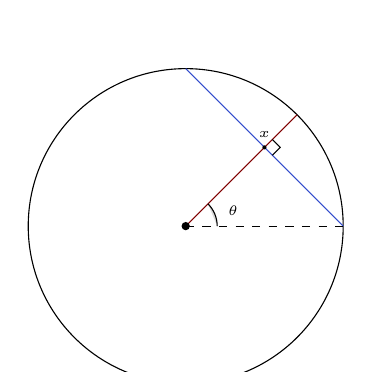
\begin{tikzpicture}[scale=2]
      \draw circle [radius = 1];
      \draw [mred] (0, 0) -- (0.707, 0.707);
      \draw [mblue] (0, 1) -- (1, 0);
      \draw [dashed] (0, 0) -- (1, 0);
      \node [circ] at (0, 0) {};
      \node [circ, fill=black, scale=0.5] at (0.5, 0.5) {};
      \node at (0.5, 0.5) [above] {{\tiny $x$}};
      \draw[fill=gray!30] (0.2,0) 
      arc[start angle=0, end angle=45, radius=0.2];
      \node at (0.3, 0.1) {{\tiny$\theta$}};
      \draw (0.55, 0.45) -- (0.6, 0.5) -- (0.55, 0.55);
    \end{tikzpicture}
\end{center}
The corresponding sample space is
\[
  \Omega = \set{(\theta, x) \mid \theta \in [0, 2 \pi),\, x \in [0,1]}.
\]
Because we choose the angle and radius uniformly and independently
on their respective intervals, we see that for any 
$[a,b] \times [c,d] \subset [0, 2 \pi) \times [0,1]$ that
\[
  \Prob([a,b] \times [c,d]) = \frac{b-a}{2 \pi} \cdot (d-c).
\]
Define a random variable $X \colon \Omega \to \R$ by
\[
  X\left((\theta, x)\right) = \text{the length of the chord corresponding
  to the pair $(\theta, x)$}.
\]
It turns out that $X(\theta,x) = 2 \sqrt{1 - x^2}$.
Now we see that
\[
  \Prob\left(X \geq \sqrt{3}\right) = 
  \Prob([0,2 \pi] \times [0,1/2]) =
  \frac{2 \pi-0}{2 \pi} \cdot (1/2-0) =
  \frac{1}{2}.
\]

\subsection{Second solution}
Now in order to choose a chord, we choose an arbitrary point inside
the circle, and consider the chord perpendicular to the radius that is
intersecting the with the point.
\begin{center}
    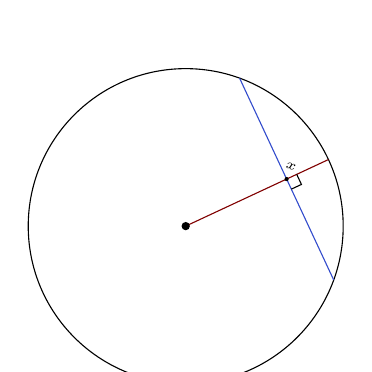
\begin{tikzpicture}[scale=2]
      \draw circle [radius = 1];
      \draw [mred, rotate=-20] (0, 0) -- (0.707, 0.707);
      \draw [mblue, rotate=-20] (0, 1) -- (1, 0);
      \node [circ] at (0, 0) {};
      \node [circ, fill=black, scale=0.5] at 
      ([rotate around={-20:(0, 0)}] 0.5, 0.5) {};
      \node[rotate=-20] at ([rotate around={-20:(0, 0)}]0.5, 0.5) 
      [above] {{\tiny $x$}};
      \draw[rotate=-20] (0.55, 0.45) -- (0.6, 0.5) -- (0.55, 0.55);
    \end{tikzpicture}
\end{center}
The corresponding sample space is
\[
  \Omega = \set{(x, y) \mid x^2 + y^2 \le 1}.
\]
Because we choose the coordinates uniformly, and independently, 
we see that for any
$[a,b] \times [c,d] \subset \Omega$ that
\[
  \Prob([a,b] \times [c,d]) = \frac{(b-a)(d-c)}{\pi},
\]
which is just the area of the rectangle divided by the area of the circle.
Define a random variable $Y \colon \Omega \to \R$ by
\[
  Y\left((x, y)\right) = \text{the length of the chord corresponding
  to the pair $(x, y)$}.
\]
It turns out that $Y(x,y) = 2 \sqrt{1 - x^2 - y^2}$.
Now the result we get is
\[
  \Prob\left(Y \geq \sqrt{3}\right) = 
  \Prob\left(\set{(x,y) \mid 2 \sqrt{1 - x^2 - y^2} \geq \sqrt{3}}\right) =
  \Prob\left(\set{(x,y) \mid x^2 + y^2 \le \frac{1}{4}}\right) =
  \frac{\frac{\pi}{4}}{\pi} =
  \frac{1}{4}.
\]

\subsection{Third solution}
Now we simply choose a chord by choosing two points on the circle, and
connecting them.
\begin{center}
      \begin{tikzpicture}[scale=2]
        \draw circle [radius = 1];
        \draw [mblue, rotate=-30] (0, -1) -- (-1, 0);
        \node [circ, fill=black, scale=0.75] at ([rotate=-30]-1, 0) {};
        \node [circ, fill=black, scale=0.75] at ([rotate=-30]0, -1) {};
      \end{tikzpicture}
\end{center}
The corresponding sample space is
\[
  \Omega = \set{(\theta_1, \theta_2) \mid \theta_1, \theta_2 \in [0,2 \pi)}.
\]
Because we choose the angles uniformly, and independently,
we see that for any
$[a,b] \times [c,d] \subset \Omega$ that
\[
  \Prob([a,b] \times [c,d]) =
  \frac{b-a}{2 \pi} \cdot \frac{d-c}{2 \pi},
\]
Define a random variable
\[
  Z\left((\theta_1, \theta_2)\right) = 
  \text{the length of the chord corresponding to the pair $(x, y)$}.
\]
As you may expect, calculating $Z$ directly this time requires
tedius geometric and trigonometric calculations.
After these calculations, we use similar methods to the ones
shown in the first two solutions, and get
\[
  \Prob\left(Z \geq \sqrt{3}\right) = 
  \frac{1}{3}.
\]

\subsection{Conclusion}
The conclusion to the paradox is that probability questions only
make sense once the sample space and measure are clearly specified.
The reason there seems to be a paradox in the first place,
is that the English expression ``suppose a chord of the circle is
chosen uniformly at random'',
seems like it determines the problem uniquely,
while in fact there are multiple ways to interpret it,
as we saw in the different solutions we gave.

\newpage

\section{Multivariate random variables}
As we saw in the beginning of \Cref{sec:random-variables},
random variables encode information about our experiments.
In some experiments, we may want to measure multiple results,
so a natural way to do it is by defining multiple random variables
$X_1,\dots,X_n \colon \Omega \to \R$,
one for each result we want to measure.
A natural question to ask may be,
what is the probability that $X_1 = X_2$?
In other words what is $\Prob(X_1 = X_2)$?
Defining multiple random variables is indeed is a good way to do
measure multiple results,
and as we will see, we call $\vec X = (X_1,\dots,X_n)$ random vectors,
but as the following example shows, we must be careful.

\begin{example}
  \label{exmp:random-vectors}
  Suppose we roll two fair dices,
  and let $X,Y \colon \Omega \to \R$ be random variables
  with the distribution $\Prob_X(i) = \Prob_Y(i) = 1/6$
  for all $i \in \set{1,2,3,4,5,6}$.
  We now want to compute $\Prob(X = Y)$.
  It may seem easy to say, well, each variable describes the roll
  of a fair die, so the probability that $X = Y$ is exactly $1/6$.
  However, just like we saw in \Cref{sec:bertrand-paradox},
  it is very important to have a perfect correspondence between
  the experiment, and our mathematical description.
  In this case, if indeed $X$ and $Y$ were the results of rolling two
  fair dice, then we would have $\Prob(X = Y) = 1/6$.
  However, suppose that we had a different experiment,
  say, we roll one fair dice, and we write the same result
  twice, where $\widetilde X$ is the first number we wrote,
  and $\widetilde Y$ is the second number we wrote.
  In this case, when we write the experiment in
  a mathematical way, unfortunately,
  we have that $\widetilde X, \widetilde Y \colon \widetilde \Omega \to \R$
  are such that $\Prob_X = \Prob_{\widetilde X}$,
  and $\Prob_Y = \Prob_{\widetilde Y}$,
  but $\Prob(X = Y) = 1$.
  This shows that random variables encode more information than their
  \textit{marginal}
  \footnote{When we consider the disribution of a random vector
  we sometimes use the phrasing ``joint distribution'',
  and when we consider the random variables as seperate from the vectors
  we sometimes use terms such as ``marginal distribution''.}
  probability distributions.
  Indeed, if we compare the sample space of both experiements,
  or consider the random variables as the functions that they are
  we could see that $X \neq Y \neq \widetilde X = \widetilde Y$,
  while $\Prob_X = \Prob_Y = \Prob_{\widetilde X} = \Prob_{\widetilde Y}$.
  This shows that the way we first described the experiment has multiple
  interpretations and does not correspond to our experiment exactly,
  unless we assume the reader \textit{implicitly} defines the sample space
  and the random variables as functions to be exactly how we want them to be.
\end{example}

\subsection{Multivariate random variables}
\begin{definition}[Multivariate random variable]
  Let $(\Omega, \mathcal F, \Prob)$ be a probability space.
  The function $\vec{X} = (X_1,\dots,X_N) \colon \Omega \to \R^N$ is said
  to be a multivariate random variable if for all $a_i < b_i$ for 
  $1 \le i \le N$ we have
  \[
    \vec{X}^{-1}\left(\prod_{i=1}^{N} (a_i, b_i)\right) =
    \set{\omega \in \Omega \mid
    a_i < X_i(\omega) < b_i,\, \forall 1 \le i \le N} \in
    \mathcal F.
  \]
  A multivariate random variable is sometimes also called a random vector.
\end{definition}

\begin{remark}
Notice that this definition also implies that $X^{-1}(A) \in \mathcal F$
for all $A \in \mathfrak B\left(\R^n\right)$.
\end{remark}

\begin{proposition}
  Let $(\Omega, \mathcal F, \Prob)$ be a probability space, 
  and let $\vec{X} = (X_1,\dots,X_N) \colon \Omega \to \R^N$. 
  Then $\vec{X}$ is a multivariate random variable if and only if 
  $X_k \colon \Omega \to \R$ is a random variable for all $1 \le k \le N$.
\end{proposition}
\begin{proof}
  Assume $\vec{X}$ is a multivariate random variable and set some $1 \le k \le N$.
  Then for all $a < b$ we have
  \[
    X_k^{-1}((a,b)) = 
    \vec{X}^{-1}\left(\R^{k-1} \times (a,b) \times \R^{n-k}\right) \in
    \mathcal F.
  \]
  Now assume $X_1,\dots,X_N$ are random variables. Then for all $a_i < b_i$
  for $1 \le i \le N$ we have
  \[
    \vec{X}^{-1}\left(\prod_{i=1}^{N} (a_i, b_i)\right) =
    \bigcap_{i=1}^{N}\set{\omega \in \Omega \mid a_i < X_i(\omega) < b_i} \in
    \mathcal F,
  \]
  where the last equality follows from the fact $\mathcal F$ is
  a $\sigma$-algebra, and $X_1,\dots,X_N$ are all random variables.
\end{proof}

\begin{definition}[Distribution of a multivariate random variable]
  Let $(\Omega, \mathcal F, \Prob)$ be a probability space, 
  and let $\vec{X} = (X_1,\dots,X_N) \colon \Omega \to \R^N$ be a multivariate
  random variable.
  The (joint) distribution of $\vec{X}$, denoted $\Prob_{\vec{X}}$ is a probability function
  on the measurable space $(\R^N, \mathfrak B(\R^n))$ defined as:
  \[
    \Prob_{\vec{X}}(A) =
    \Prob(\vec{X} \in A), \quad
    \forall A \in \mathfrak B(\R^N).
  \]
\end{definition}

\begin{remark}
  The function $\Prob_{X_k}$ denotes the distribution of the random
  variable $X_k$ and is called the partial distribution of $X_k$.
  We see that the distribution $\Prob_{\vec{X}}$ of a random vector uniquely
  defines the partial distributions $\Prob_{X_1},\dots,\Prob_{X_N}$
  because
  \[
    \Prob_{X_k} =
    \Prob_{\vec{X}}\left(\R^{k-1} \times A \times \R^{N-k}\right),
    \quad \forall A \in \mathfrak B.
  \]
  As we saw in \Cref{exmp:random-vectors},
  the opposite is not true -
  the partial distributions do not determine the joint distribution
  uniquely.
\end{remark}

\begin{exercise}
  Suppose there are
  $3$ red balls, $4$ white balls, and $5$ blue balls in a vase.
  Three balls are arbitrarily drawn out of the vase.
  Denote the number of red balls drawn by $X$, and the number of white
  balls drawn by $Y$.
  What is the distribution of the random vector $(X,Y)$?
\end{exercise}
\begin{solution}
  We see that
  \[
    \Omega = \set{(i,j) \mid i,j \geq 0 \stand i + j \le 3},
  \]
  where $i$ denotes the number of red balls drawn, and $j$ the number
  of white balls drawn.
  From a simple combinatorial arguments we get
  \[
    \Prob_{(X,Y)}\left((i,j)\right) =
    \frac{\binom{3}{i}\binom{4}{j}\binom{5}{3-i-j}}{\binom{12}{3}}.
  \]
\end{solution}

\begin{definition}[Cumulative distribution function]
  Let $(\Omega, \mathcal F, \Prob)$ be a probability space, 
  and let $\vec{X} = (X_1,\dots,X_N) \colon \Omega \to \R^N$ be a random vector.
  The cumulative distribution function of $\vec{X}$, denoted $F_{\vec{X}}$, 
  is the function $F_{\vec{X}} \colon \R^N \to [0,1]$ defined as
  \[
    F_{\vec{X}}(a_1,\dots,a_N) =
    \Prob(X_i \le a_i,\, \forall 1 \le i \le N) =
    \Prob_{\vec{X}}\left(\prod_{i=1}^{N}(-\infty,a_i]\right).
  \]
\end{definition}

\begin{proposition}[Properties of the CDF]
  \label{prop:rv-properties-of-cdf}
  Let $(\Omega, \mathcal F, \Prob)$ be a probability space, 
  and let $\vec{X} = (X_1,\dots,X_N) \colon \Omega \to \R^N$ be a random vector.
  Then
  \begin{enumerate}
    \item[(1)] The function $F_{\vec{X}}$ is increasing in each coordinate.
    \item[(2)] The function $F_{\vec{X}}$ is right-continuous in each 
      coordinate.
    \item[(3)] Fix $a_1,\dots,a_{k-1},a_{k+1},\dots,a_N \in \R$, then
      we have $\lim_{a_k \to -\infty}{F_X(a_1,a_2,\dots,a_N)} = 0$.
    \item[(4)] Denote $X^k = (X_1,\dots,X_{k-1},X_{k+1},\dots,X_N)$ the random 
    vector with the $k$th coordinate removed. 
    Then for every choice $a_1,\dots,a_{k-1},a_{k+1},\dots,a_N \in \R$
    we have
    \[
      \lim_{a_k \to \infty} F_{\vec{X}}(a_1,a_2,\dots,a_N) =
      F_{X^k}(a_1,\dots,a_{k-1},a_{k+1},\dots,a_N).
    \]
    In particular
    \[
      \lim_{a_1,\dots,a_N \to \infty} F_{\vec{X}}(a_1,a_2,\dots,a_N) = 1.
    \]
  \end{enumerate}
\end{proposition}
\begin{proof}
  The proofs are quite straightforward.
  It is important to remember that when trying to prove
  that an increasing function $f$ converges to infinity, it suffices
  to prove that $f(a_n) \to \infty$ for any $a_n \to \infty$ you choose.
  This lemma is more useful in this course than other courses due
  to the nature of distribution functions (they are always increasing).
\end{proof}

\begin{remark}
  The following two theorems are generalizations of
  \Cref{thm:FcharacterizesP} and \Cref{thm:FcharacterizesPtwo}
  respectively.
  They allow us to conclude that there exists a bijection between all random
  vectors' distributions and
  functions that satisfy the $4$ properties from
  \Cref{prop:rv-properties-of-cdf}.
\end{remark}
\begin{theorem}
  Every cumulative distribution function corresponds to a unique distribution.
  In other words,
  if $(\Omega, \mathcal F, \Prob)$ and $(\Omega', \mathcal F', \Prob')$
  are two probability spaces, and $\vec{X} \colon \Omega \to \R^N$,
  $\vec{Y} \colon \Omega' \to \R^N$ are two random variable, then
  \[
    F_{\vec{X}} = F_{\vec{Y}} \iff 
    \Prob_{\vec{X}} = \Prob_{\vec{Y}}
  \]
\end{theorem}
\begin{theorem}
  Let $F \colon \R^N \to [0,1]$ be a function that satisfies all $4$
  properties in \Cref{prop:rv-properties-of-cdf}.
  Then there exists a probability space 
  $(\Omega, \mathcal F, \Prob)$ and a random vector
  $\vec{X} \colon \Omega \to \R^N$ such that $F_{\vec{X}} = F$.
\end{theorem}

\subsection{Theory of random vectors}

\begin{definition}[Discrete random vector]
  Let $(\Omega, \mathcal F, \Prob)$ be a probability space, 
  and let $\vec{X} = (X_1,\dots,X_N) \colon \Omega \to \R^N$ be a random vector.
  Then $\vec{X}$ is said to be a discrete random vector if there
  exists a countable set $B \subset \R^\N$ such that
  $\Prob(\vec{X} \in B) = 1$.
\end{definition}

\begin{proposition}
  Let $(\Omega, \mathcal F, \Prob)$ be a probability space, 
  and let $\vec{X} = (X_1,\dots,X_N) \colon \Omega \to \R^N$ be a random vector.
  Then $\vec{X}$ is a discrete random vector if and only if $X_k$ is a discrete
  random variable for all $1 \le k \le N$.
\end{proposition}
\begin{proof}
  Assume that $\vec{X} = (X_1,\dots,X_N)$ is a discrete random vector.
  Then there exists a countable set $B \subset \R^N$ such that
  \[
    \Prob_{\vec{X}}(B) = 1.
  \]
  Let $1 \le k \le N$. Consider the set $B_k = \pi_k(B)$ where $\pi_k$ is the
  projection on the $k$th coordinate. It is clear that $B_k$ is countable
  and also
  \[
    1 \geq
    \Prob(X_1 \in B_k) =
    \Prob\left((X_1,\dots,X_N) \in B_k \times \R^{N-1}\right) \geq
    \Prob(\vec{X} \in B) =
    1,
  \]
  where the last inequality follows from the fact
  that $B \subset B_k \times \R^{N-1}$.
  Thus we got that for all $1 \le k \le N$ that $X_k$ is discrete.
  Now suppose that $X_1,\dots,X_N$ are discrete random variables.
  Then exist countable sets $B_1,\dots,B_N$ such that 
  $\mathbf (X_k \in B_k) = 1$ for all $1 \le k \le N$.
  The set $B = B_1 \times \cdots \times B_N$ is countable and it is clear that
  $\Prob(\vec{X} \in B) = 1$ as wanted which completes the proof.
\end{proof}

\begin{remark}
  Notice that the above proposition proves that given a discrete random
  vector $\vec{X} = (A_i)_{i=1}^{N}$, for any subsequence $\{i_j\}_{j=1}^{k}$ of 
  $\{i\}_{i=1}^N$ that $\vec{X} = (A_{i_j})_{j=1}^k$ is also a discrete random
  vector.
\end{remark}

\begin{definition}[Continuous random vector]
  Let $(\Omega, \mathcal F, \Prob)$ be a probability space, 
  and let $\vec{X} = (X_1,\dots,X_N) \colon \Omega \to \R^N$ be a random vector.
  Then $\vec{X}$ is called a continuous random vector if 
  $F_{\vec{X}}$ is a continuous function.
\end{definition}

\begin{remark}
  As in the case of a random variable, if $\vec{X} \colon \Omega \to \R^N$ is
  a continuous random vector, 
  then $\Prob(\vec{X} = a) = 0$ for all $a \in \R^N$.
\end{remark}

\begin{remark}
  The full theory of continuous random vectors is outside the scope of this
  course and we will only focus on absolutely continuous random vectors.
\end{remark}

\begin{definition}[Absolutely continuous random vector]
  Let $(\Omega, \mathcal F, \Prob)$ be a probability space, 
  and let $\vec{X} = (X_1,\dots,X_N) \colon \Omega \to \R^N$ be a random vector.
  Then $\vec{X}$ is said to be absolutely continuous if there
  exists an integrable 
  function $f \colon \R^N \to [0,\infty)$ such that 
  \[
    \int_{\R_N} f(x) \dx = 1,
  \]
  and such that for all $a \in \R^N$ we have:
  \[
    F_{\vec{X}}(a) = 
    \Prob_{\vec{X}}\left(\prod_{i=1}^{N} (-\infty,a_i]\right) =
    \int_{\prod_{i=1}^{N} (-\infty,a_i]} f(y_1,\dots,y_N)\dif (y_1,\dots,y_N).
  \]
  In this case, we call $f_{\vec{X}}$ the probability density function of 
  $\vec{X}$, or the PDF of $\vec X$ for short.
\end{definition}

\begin{remark}
  Similarly to the theory of random variables,
  this definition implies that for any $A \subset \R^N$,
  such that $f \cdot \ind_A$ is an integrable function,
  we get
  \[
    \Prob_{\vec{X}}(A) = 
    \int_{A} f(y_1,\dots,y_N)\dif (y_1,\dots,y_N).
  \]
\end{remark}

\begin{remark}
  Let $(X,Y)$ be a continuous random vector with distribution function $F(x,y)$.
  Assume that $F$ piecewise twice continuously differentiable.
  Then $f(x,y) = \frac{\partial^2 F}{\partial x \partial y}(x,y)$.
  Of course this can be generalized to $n$-dimensional random vectors
  as well.
\end{remark}

\begin{remark}
  Our main tool for dealing with integrals in $\R^n$ is called
  Fubini's theorem.
  We are going to use the version of the theorem that generalizes
  Fubini's theorem from analysis $2$ to functions on $\R^n$.
\end{remark}

\begin{theorem}[Fubini's theorem]
  Let $f \colon A \times B \to \R$ be Riemann integrable, where 
  $A,B \subset \R$ are closed sets.
  For all $x \in A$ define the function $f_x \colon B \to \R$ by
  $f_x(y) = f(x,y)$.
  If for all $x \in A$ the function $f_x$ is Riemann integrable on $B$,
  then
  \[
    \int_{A \times B} f(x,y) \dif (x,y) =
    \int_{A}\left(\int_{B} f_x(y) \dy\right) \dx.
  \]
  Similarly, for each $y \in B$ we define the function 
  $f^y \colon A \to \R$ by $f^y(x) = f(x,y)$.
  If for all $y \in B$ the function $f^y$ is Riemann integrable on $A$,
  then
  \[
    \int_{A \times B} f(x,y) \dif(x,y) =
    \int_{B}\left(\int_{A} f^y(x) \dx\right) \dy.
  \]
\end{theorem}

\begin{exercise}
  Let $(X,Y)$ be a random vector with a probability density function
  given by
  \[
    f_{(X,Y)}(x,y) =
    \begin{cases}
      c(2x+y^2) & 0 \le x \le 1 \stand 0 \le y \le 2, \\
      0 &\text{otherwise}.
    \end{cases}
  \]
  \begin{enumerate}
    \item[(1)] Find the value of $c$.
    \item[(2)] Calculate $\Prob(X + Y \le 1)$.
  \end{enumerate}
\end{exercise}
\begin{solution}
  \begin{enumerate} \phantom{}
    \item[(1)]
  In order to find $c$ we can use the fact that 
  $\int_{\R^2} f_{(X,Y)}(x,y) \dif (x,y) = 1$.
  From Fubini's theorem we get that
  \begin{align*}
    1 &= \int_{\R^2} f_{(X,Y)}(x,y) \dif(x,y)
    = \int_{0}^{1}\left(\int_{0}^{2} c(2x + y^2) \dy\right) \dx
    = c \int_{0}^{1} \left[2xy + \frac{y^3}{3}\right]\biggr\vert^2_0 \dx \\
    &= c \int_{0}^{1} 4x + \frac{8}{3} \dx
    = \frac{14}{3}c,
  \end{align*}
  which implies that $c = \frac{3}{14}$.
    \item[(2)]
  In order to find $\Prob(X + Y \le 1)$,
  we need to understand that the function is only different than zero
  on the rectangle $R = [0,1] \times [0,2]$.
  This means that we need to find the integral of $f_X$ on 
  $T = R \cap \set{(x,y) \mid x + y \le 1}$. 
  Using Fubini's theorem we get
  \begin{align*}
    \Prob(X + Y \le 1) &= \int_{T}f_{(X,Y)} (x,y) \dif (x,y)
    = \frac{3}{14} \int_{0}^{1} 
    \left(\int_{0}^{1-x} 2x + y^2 \dy\right) \dx \\
    &= {\frac{3}{14}}\int_{0}^{1}2x(1-x)+{\frac{(1-x)^{3}}{3}} \dx
    = {\frac{5}{56}}.
  \end{align*}
  \end{enumerate}
\end{solution}

\begin{theorem}\label{thm:randvec}
  Let $(\Omega, \mathcal F, \Prob)$ be a probability space, 
  and let $\vec{X} = (X_1,\dots,X_N) \colon \Omega \to \R^N$ be an absolutely
  continuous random vector with a probability density function 
  $f_{\vec{X}} \colon \R^N \to [0,\infty)$.
  Then, for all $1 \le k \le N$,
  the random variable $X_k$ is absolutely continuous
  with a probability density function
  \[
    f_{X_{k}}(a) = 
    \int_{\R^{N-1}} 
    f_{\vec{X}}(x_{1},\dots,x_{k-1},a,x_{k+1},\dots,x_{N})
    \dif (x_{1},\ldots,x_{k-1},x_{k+1},\dots,x_{N}).
  \]
\end{theorem}

\begin{definition}[Volume]
  Let $A \subset \R^N$ be a set. We define the volume of $A$ as such
  \[
    \Vol(A) = \int_{\R^N} \mathbbm{1}_A(x) \dx.
  \]
\end{definition}

\begin{definition}[Uniform distribution]
  Let $\vec{X} \colon \Omega \to \R^N$ be a random vector, 
  and $B \subset \R^N$ an open or closed set with a well defined, finite volume.
  The random vector $\vec{X}$ is said to distribute uniformly on $B$, and
  we write $\vec{X} \sim U(B)$,
  if $\vec{X}$ is absolutely continuous with a 
  probability density function
  \[
    f_{\vec{X}}(x) =
    \begin{cases}
      \frac{1}{\Vol(B)} &x \in B, \\
      0 &\text{otherwise}.
    \end{cases}
  \]
\end{definition}

% \begin{remark}
%   Recall that in the case of random variables,
%   if $X$ is absolutely continuous then
%   $F_X(a) = \int_{-\infty}^{a} f_X(y) \dy$,
%   which allowed us to compute $F_X$ from $f_X$,
%   and by the fundamental theorem of calculus,
%   we also got that $F_X'(a) = f_X(a)$.
%   In the multivariate case, if $\vec X$ is an absolutely continuous
%   random vector, then we still have 
%   $F_{\vec X}(a) = \int_{\prod_{i=1}^{N} (-\infty,a_i]} f(y_1,\dots,y_N)\dif (y_1,\dots,y_N)$,
%   and the following proposition will show us how to compute
%   $f_{\vec X}$ from $F_{\vec X}$.
% \end{remark}
%
% \begin{proposition}
%   Let $\vec X \colon \Omega \to \R^N$ be an absolutely continuous
%   random variable with a probability density function $f_{\vec X}$
% \end{proposition}

\begin{definition}[Independence]
  Let $X_1,\dots,X_N \colon \Omega \to \R$ be random variables.
  The variables $X_1,\dots,X_N$ are said to be independent if
  for all $A_1,\dots,A_N \in \mathfrak B$ we have
  \[
    \Prob(X_1 \in A_1, \dots, X_N \in A_N) =
    \prod_{i=1}^{N} \Prob(X_i \in A_i).
  \]
\end{definition}

\begin{remark}
  Equivalently,
  we can write that $X_1,\dots,X_N$ are independent if
  for all Borel measurable sets $A_1,\dots,A_N$ we have
  \[
    \Prob\del{\bigcap_{i=1}^{N} \set{X_i \in A_i}} =
    \prod_{i=1}^{N} \Prob(X_i \in A_i).
  \]
  This means that $X_1,\dots,X_N$ are independent if and only if
  for all Borel measurable sets $A_1,\dots,A_N$ the events
  $(\set{X_i \in A_i})_{i=1}^{N}$ are independent.
  In terms of distributions, this means that
  \[
    \Prob_{\vec X}(A_1 \times \cdots \times A_N) =
    \prod_{i=1}^{N} \Prob_{X_i}(A_i).
  \]
  Wait.
  This formula shows that
  when $X_1,\dots,X_N$ are independent variables,
  the partial distributions $\Prob_{X_i}$ \textit{do} determine
  $\Prob_{\vec X}$ uniquely.
  If you forgot why this is so surprising,
  recall \Cref{exmp:random-vectors}.
\end{remark}

\begin{proposition}
  \label{prop:independent-rv-equivalencies}
  Let $X_1,\dots,X_N \colon \Omega \to \R$ be random variables,
  and denote $\vec X = (X_1,\dots,X_N)$.
  Then
  \begin{enumerate}
    \item[(1)] If $X_1,\dots,X_N$ are independent,
      then $F_{\vec X}(a_1,\dots,a_N) = \prod_{i=1}^{N} F_{X_i}(a_i)$
      for all $a_1,\dots,a_N \in \R$.
    \item[(2)] If $X_1,\dots,X_N$ are independent,
      and $\vec X$ is absolutely continuous,
      then $f_{\vec X}(a_1,\dots,a_N) = \prod_{i=1}^{N} f_{X_i}(a_i)$
      for all $a_1,\dots,a_N \in \R$.
  \end{enumerate}
\end{proposition}
\begin{remark}
  In fact both $(1)$ and $(2)$ are if and only if statements.
\end{remark}

\begin{example}
  Let $X$ and $Y$ be two random variables so that
  $\Prob(X = i) = \Prob(Y = i) = 1/2$ for $i \in \set{0,1}$.
  Then $X$ and $Y$ are independent if and only if
  $\Prob(X = i, Y = j) = 1/4$ for any $i,j \in \set{0,1}$.
  Recall that once we know the partial distributions $\Prob_X$ and $\Prob_Y$,
  and that $X$ and $Y$ are independent, then we can compute $\Prob_{(X,Y)}$.
\end{example}

\begin{exercise}
  Let $X_1 \sim \Exp(\lambda_1)$ and $X_2 \sim \Exp(\lambda_2)$,
  and suppose that $X_1$ and $X_2$ are independent.
  Find $\Prob(X_2 > X_1)$.
\end{exercise}
\begin{solution}
  We know that $X_i$ is absolutely continuous with
  \[
    f_{X_i}(x) =
    \begin{cases}
      \lambda_i e^{-\lambda_i x} &x \geq 0, \\
      0 &x < 0,
    \end{cases}
  \]
  for all $i \in \set{1,2}$.
  Since $X_1$ and $X_2$ are independent,
  by \Cref{prop:independent-rv-equivalencies} we conclude that
  \[
    f_{(X_1,X_2)}(x,y) =
    f_{X_1}(x) f_{X_2}(y) =
    \begin{cases}
      \lambda_1 \lambda_1 e^{\lambda_1 \lambda_2 x y} &x \geq 0 \stand y \geq 0, \\
      0 &\text{otherwise}.
    \end{cases}
  \]
  Therefore, we have that
  \[
    \Prob(X_2 > X_1) =
    \int_{\set{(x,y) \mid y > x}} f_{(X_1,X_2)}(x,y) \dif(x,y).
  \]
  However, we can see that the only part of $\set{(x,y) \mid y > x}$
  where $f_{(X_1,X_2)}(x,y)$ does not vanish
  is $\set{(x,y) \mid y > x > 0}$,
  so we can use Fubini's theorem to conclude that
  \begin{align*}
    \Prob(X_2 > X_1) &=
    \int_{\set{(x,y) \mid y > x}} f_{(X_1,X_2)}(x,y) \dif(x,y) =
    \int_{0}^{\infty} \del{\int_{x}^{\infty} \lambda_1 \lambda_1 e^{\lambda_1 \lambda_2 x y} \dy} \dx \\ &=
    \int_{0}^{\infty} \lambda_1 e^{-\lambda_1 x} \del{\int_{x}^{\infty} \lambda_2 e^{-\lambda_2 y} \dy} \dx =
    \int_{0}^{\infty} \lambda_1 e^{-\lambda_1 x} \left[-e^{-\lambda_2 y}\right] \biggr\vert^{\infty}_{x} \dx \\ &=
    \lambda_1 \int_{0}^{\infty} e^{\lambda_1 \lambda_2 x^2} \dx =
    \frac{\lambda_1}{\lambda_1 + \lambda_2}.
  \end{align*}
\end{solution}


\begin{definition}[Measure]
  \label{def:measure}
  Let $(X, \Sigma)$ be a measurable space.
  A function $\mu \to [0,\infty]$ is called a measure if the following
  conditions hold
  \begin{enumerate}
    \item[(1)] $\mu(\emptyset) = 0$;
    \item[(2)] For all countable collections $\{E_{k}\}_{k=1}^{\infty }$ of
          pairwise disjoint sets in $\Sigma$ we have
          \[ \mu \left(\bigsqcup _{k=1}^{\infty }E_{k}\right) =
             \sum _{k=1}^{\infty }\mu (E_{k}). \]
  \end{enumerate}
\end{definition}

\begin{remark}
  Condition $(2)$ in \Cref{def:measure} is called $\sigma$-additivity.
\end{remark}

\begin{remark}
  Note that if $(\Omega,\mathcal F,\Prob)$ is a probability space,
  then $\Prob$ is a measure on $(\Omega,\mathcal F)$.
  Conversely, any probability function $\Prob \colon \Omega \to [0,1]$
  is a measure on $(\Omega,\mathcal F)$, so that $\mu(\Omega) = 1$.
  That is why in measure theory, a probability function is called
  a probability measure.
\end{remark}

\begin{definition}[Atom]
  \label{def:atom}
  Let $(X, \Sigma)$ be a measurable space,
  and let $\mu $ be a measure on that space.
  A set $A \subset X$ in $\Sigma$ is called an atom, if
  the following conditions holds:
  \begin{enumerate}
    \item[(1)] $\mu (A) > 0$.
    \item[(2)] For any measurable set $B \subset A$,
      either $\mu(B) = 0$, or $\mu(A \setminus B) = 0$.
  \end{enumerate}
\end{definition}

\begin{remark}
  The intuition for \Cref{def:atom} is that it cannot be split into
  smaller measurable sets (with measure greater than zero),
  just like an atom.
  This definition is not going to be very important from now on,
  but I still included it because it appears from time to time
  when talking about discrete random vectors.
\end{remark}

\begin{remark}
  Note that in the case of a distribution
  $\Prob_{\vec X} \colon \mathfrak B(\R^N) \to \R$,
  its atoms must be singletons.
\end{remark}

\begin{remark}
  Similarly to \Cref{thm:mixed-rv},
  we can decompose every random vector $\vec X \colon \Omega \to \R^N$
  to the sum of a discrete and a continuous random vector.
  The proof of this decomposition is outside the scope of the course,
  but we will still give the formal statment.
\end{remark}

\begin{theorem}
  Let $\vec X \colon \Omega \to \R^N$ be a random vector,
  and let $\set{\set{a_i}}_{i=1}^{\infty} \subset \R^N$ be the atoms of
  the distribution $\Prob_{\vec X}$.
  Then there exists a discrete and continuous distribution
  functions $F_{\vec X}^d$ and $F_{\vec X}^c$ respectively,
  so that
  $
    F_{\vec X} =
    \alpha F_{\vec X}^{d} + (1 - \alpha) F_{\vec X}^{c}
  $.
\end{theorem}

\begin{remark}
  We can generalize \Cref{prop:function-of-rv}
  to random vectors.
  If $\vec X \colon \Omega \to \R^N$ is a random vector,
  and $h \colon \R^N \to \R^M$ is a measurable function,
  then $\vec Y = h(\vec X)$ is a random vector.
  We also want to generalize \Cref{prop:distribution-of-Y}
  and describe $F_{\vec Y}$ with $F_{\vec X}$.
  However, instead of talking about the general case,
  in this course, we will only talk about what happens
  in the cases of a few simple functions,
  all of which are of the form $h \colon \R^n \to \R$.
\end{remark}

\begin{example}[Maximum of two variables]
  Let $X,Y \colon \Omega \to \R$ be random variables,
  and define $Z \colon \Omega \to \R$ by $Z = \max\set{X,Y}$.
  Note that $h \colon (x,y) \mapsto \max(x,y)$ is continuous
  and therefore it is measurable, so $Z = h(X,Y)$ is a random variable.
  Our goal is to compute $F_Z$ in terms of the distributions of $X$
  and $Y$.
  We get that
  \[
    F_{Z}(a) =
    \Prob(Z \le a) =
    \Prob(X \le a, Y \le a) =
    F_{(X,Y)}(a,a).
  \]
  For example if $X \sim U([0,1])$, $Y \sim U([0,1])$,
  and $X$ and $Y$ are independent,
  then
  \[
    F_{Z}(a) =
    F_{(X,Y)}(a,a) =
    F_X(a) F_Y(a) =
    \begin{cases}
      0 &a < 0, \\
      a^2 &0 \le a \le 1, \\
      1 &a > 0, \\
    \end{cases}
  \]
  where the second transition follows from the fact $X$ and $Y$
  are independent.
\end{example}

\begin{example}[Minimum of two variables]
  Let $X,Y \colon \Omega \to \R$ be random variables,
  and define $Z \colon \Omega \to \R$ by $Z = \min\set{X,Y}$.
  Note that $h \colon (x,y) \mapsto \min(x,y)$ is continuous
  and therefore it is measurable, so $Z = h(X,Y)$ is a random variable.
  Our goal is to compute $F_Z$ in terms of the distributions of $X$
  and $Y$.
  We get that
  \begin{align*}
    F_{Z}(a) &=
    \Prob(Z \le a) =
    \Prob(X \le a \stor Y \le a) \\ &=
    \Prob(X \le a) + \Prob(Y \le a) - \Prob(X \le a, Y \le a) =
    F_X(a) + F_Y(a) - F_{(X,Y)}(a,a).
  \end{align*}
  For example if $X \sim U([0,1])$, $Y \sim U([0,1])$,
  and $X$ and $Y$ are independent,
  then
  \[
    F_{Z}(a) =
    F_X(a) + F_Y(a) - F_{(X,Y)}(a,a) =
    F_X(a) + F_Y(a) - F_X(a) F_Y(a) =
    \begin{cases}
      0 &a < 0, \\
      2a - a^2 &0 \le a \le 1, \\
      1 &a > 0, \\
    \end{cases}
  \]
  where the second transition follows from the fact $X$ and $Y$
  are independent.
\end{example}

\begin{example}[Sum of two independent variables]
  \label{exmp:sum-of-rv}
  Let $X,Y \colon \Omega \to \R$ be independent random variables,
  and define $Z = X + Y$.
  Note that $h \colon (x,y) \mapsto x + y$ is continuous
  and therefore it is measurable, so $Z = h(X,Y)$ is a random variable.
  Our goal is to compute $F_Z$ in terms of the distributions of $X$
  and $Y$.
  First, assume that $X$ and $Y$ are discrete with
  support $\set{a_i}_{i=1}^{\infty}$ and $\set{b_i}_{i=1}^{\infty}$
  respectively.
  We get that
  \[
    F_{Z}(a) =
    \Prob(X + Y \le a) =
    \sum_{i=1}^{\infty} \Prob(X + Y \le a, X = a_i) =
    \sum_{i=1}^{\infty} \Prob(Y \le a - a_i, X = a_i).
  \]
  Since $X$ and $Y$ are independent we conclude that
  \[
    F_{Z}(a) =
    \sum_{i=1}^{\infty} \Prob(Y \le a - a_i) \Prob(X = a_i) =
    \sum_{i=1}^{\infty} F_Y(a - a_i) \Prob_X(a_i).
  \]
  Now assume that $X$ and $Y$ are absolutely continuous,
  so $f_{(X,Y)} = f_X(x) f_Y(y)$, and thus
  \begin{align*}
    F_{X+Y}(a) &=
    \Prob(X + Y \le a) =
    \int_{\set{(x,y) \mid x + y \le a}} f_{(X,Y)} \dif (x,y) =
    \int_{\set{(x,y) \mid x + y \le a}} f_X(x) f_Y(y) \dx\dy\\ &=
    \int_{-\infty}^{\infty} \del{ \int_{-\infty}^{a - x}
      f_X(x) f_Y(y) \dy} \dx =
    \int_{-\infty}^{\infty} f_X(x) \del{ \int_{-\infty}^{a - x}
      f_Y(y) \dy} \dx \\ &=
    \int_{-\infty}^{\infty} f_X(x) F_Y(a - x) \dx.
  \end{align*}
  Note that in both cases we got that $F_{X+Y}(a)$
  is a sum (or integral) over one function valued at $x$,
  and another function valued at $a - x$.
  This type of expression is fundamental in all kinds
  of fields of mathematics, most prominently in Fourier analysis,
  and it is called a \textit{convolution}.
\end{example}

\begin{definition}[Convolution]
  Let $f,g \colon \R \to [0,\infty)$.
  The convolution of $f$ and $g$, denoted
  $f * g \colon \R \to [0,\infty)$,
  is the function
  \[
    (f * g)(a) := \int_{-\infty}^{\infty} f(x) g(a - x) \dx.
  \]
\end{definition}
\begin{remark}
  We can also define convolutions for $f,g \colon \R \to \R$
  such that $\abs{f}$ and $\abs{g}$ are integrable.
  These type of functions are called $\mathcal L^1(\R)$ functions.
\end{remark}
\begin{remark}
  The convolution operator is well defined,
  commutative ($f * g = g * f$),
  and associative ($(f * g) * h = f * (g * h)$).
\end{remark}
\begin{remark}
  The computations in \Cref{exmp:sum-of-rv} show
  that for random variables $X,Y \colon \Omega \to \R$
  we have $F_{X+Y} = f_X * F_Y = f_Y * F_X$,
  and $f_{X+Y} = f_X * f_Y$. 
  Also note that the fact $f_{X+Y} = f_X * f_Y$,
  shows that $X+Y$ is absolutely continuous.
\end{remark}

\begin{example}
  Let $X,Y \sim U([0,1])$ be independent random variables.
  Then
  \[
    f_{X+Y}(a) =
    (f_{X} * f_{Y})(a) =
    \int_{-\infty}^{\infty} f_X(x) f_Y(x - a) \dx =
    \int_{0}^{1} f_Y(x - a) \dx =
    \abs{[0,1] \cap [a-1,a]}.
  \]
  By a matter of calculation
  \[
    f_{X+Y}(a) =
    \begin{cases}
      0 & a \le 0, \\
      a & a \le a \le 1, \\
      2 - a & 1 \le a \le 2, \\
      0 & a \geq 2.
    \end{cases}
  \]
\end{example}

\begin{exercise}[The Rayleigh distribution]
  Let $(X,Y) \colon \Omega \to \R^2$
  be an absolutely continuous random vector with
  $f_{(X,Y)}(x,y) = \frac{1}{2\pi} e^{-\frac{x^2 + y^2}{2}}$.
  Denote $R = \sqrt{X^2 + Y^2}$,
  and compute $f_R(r)$
\end{exercise}
\begin{solution}
  We have that
  \[
    F_R(r) =
    \Prob(\sqrt{X^2 + Y^2} \le a) =
    \Prob(X^2 + Y^2 \le a^2) =
    \int_{\set{(x,y) \mid |(x,y)| \le a}} f_{(X,Y)}(x,y) \dif(x,y).
  \]
  By the change of variables theorem
  \[
    F_R(r) =
    \int_{0}^{2\pi} \dtheta \int_{0}^{r}
    \frac{1}{2\pi} e^{-\frac{r^2}{2}} \cdot r \dr =
    \int_{0}^{r} e^{-\frac{r^2}{2}} \cdot r \dr =
    \begin{cases}
      1 - e^{-r^2/2} & r \geq 0, \\
      0 &\text{otherwise}.
    \end{cases}
  \]
  Therefore,
  \[
    f_R(r) =
    F_R'(r) =
    \begin{cases}
      r e^{-r^2/2} & r \geq 0, \\
      0 &\text{otherwise}.
    \end{cases}
  \]
  This distribution is called the Rayleigh distribution
  with parameter $\sigma = 1$.
\end{solution}

\newpage

\section{Expectation of random vectors, covariance and correlation}
\subsection{Expectation}
\begin{remark}[Expectation of random vectors]
A natural extension of expectation to random vectors is to set
\[
  \E[\vec{X}] =
  \int_{\R^N} \vec y f_{\vec{X}}(y) \dif \vec y =
  \int_{\mathbb{R}^{N}} 
  \left(y_{1},\cdots,y_{N}\right)
  f_{\vec{X}} (y_{1},\cdot\cdot\cdot,y_{N})
  \dif (y_{1},\cdot\cdot\cdot\cdot,y_{N}).
\]
Recall that an intergal of vectors is defined as the vector of the
integrals
\[
  \E[\vec{X}] =
  \left(
  \int_{\mathbb{R}^{N}} 
  y_1 f_{\vec{X}} (y_{1},\cdot\cdot\cdot,y_{N})
  \dif (y_{1},\cdot\cdot\cdot\cdot,y_{N})
  ,\dots,
  \int_{\mathbb{R}^{N}} 
  y_N f_{\vec{X}} (y_{1},\cdot\cdot\cdot,y_{N})
  \dif (y_{1},\cdot\cdot\cdot\cdot,y_{N})
  \right).
\]
Now we can consider the first coordinate and using Fubini's theorem we
get
\begin{align*}
  \int_{\mathbb{R}^{N}} 
  y_1 f_{\vec{X}} (y_{1},\cdot\cdot\cdot,y_{N})
  \dif (y_{1},\cdot\cdot\cdot\cdot,y_{N}) &=
  \int_{\mathbb{R}}
  \left[\int_{\mathbb{R}^{N-1}}
  y_{1}f_{\vec{X}}(y_{1},\dots,y_{N}) \dif (y_{2},\dots, y_{N})\right] \dy_{1} \\
  &= \int_{\mathbb{R}} y_1
  \left[\int_{\mathbb{R}^{N-1}}
  f_{\vec{X}}(y_{1},\dots,y_{N}) \dif (y_{2},\dots, y_{N})\right] \dy_{1} \\
  &= \int_{\mathbb{R}} y_1
  f_{X_1}(y_1) \dy_1 \\
  &= \E[X_1],
\end{align*}
where the second to last equality follows from \Cref{thm:randvec}.
This leads us to the following definition.
\end{remark}

\begin{definition}[Expectation]
  Let $\vec{X} \colon \Omega \to \R^N$ be a random vector such
  that $\E[X_i]$ is well defined and finite for all $1 \le i \le N$.
  Then we define
  \[
    \E[X] = (\E[X_1],\dots,\E[X_n]).
  \]
\end{definition}

\begin{proposition}
  \label{prop:vector-lotus}
  Let $\vec{X} \colon \Omega \to \R^N$ be a random vector, and let
  $h \colon \R^N \to \R$ be a measurable function such that the
  random variable $\abs{h(\vec{X})}$ has a finite expectation.
  Then if $\vec{X}$ is absolutely continuous with a probability density
  function $f_{\vec{X}}$, then
  \[
    \E[h(\vec{X})] =
    \int_{\R^N} h(\vec{y}) f_{\vec{X}}(\vec{y}) \dif\vec{y}.
  \]
  And if $\vec{X}$ is a discrete random vector with
  $\supp(\Prob_{\vec{X}}) = (\vec{a}^i)_{i \geq 1}$, then
  \[
    \E[h(\vec{X})] =
    \sum_{i=1}^{\infty} h(\vec{a}^i) \Prob_{\vec{X}}(\vec{a}^i).
  \]
\end{proposition}
\begin{remark}
  Note that \Cref{prop:vector-lotus} is
  a generalization of the law of the unconscious statistician
  we saw in \Cref{prop:lotus-discrete} and \Cref{prop:lotus-continuous}. 
\end{remark}

\begin{corollary}[Linearity of expectation]
  Let $X,Y \colon \Omega \to \R$ be two random variables and $a,b \in \R$.
  Then
  \[
    \E[aX + bY] = a \E[X] + b \E[Y].
  \]
\end{corollary}
\begin{proof}
  The idea is using \Cref{prop:vector-lotus} with
  the function $h(x,y) = ax + by$.
\end{proof}

\begin{corollary}
  \label{cor:exy-exey}
  Let $X,Y \colon \Omega \to \R$ be two random variables.
  If $X$ and $Y$ are independent then
  \[
    \E[XY] = \E[X] \E[Y].
  \]
  This implies, 
  \[
    \Var(X + Y) = \Var(X) + \Var(Y).
  \]
  However, the converse is not always true.
\end{corollary}
\begin{proof}
  The idea for the first part is using \Cref{prop:vector-lotus} with
  the function $h(x,y) = xy$.
  The second part follows by applying the first part and linearity
  of expectation.
\end{proof}

\begin{remark}
  As mentioned in the proof of \Cref{cor:exy-exey},
  the equation $\Var(X + Y) = \Var(X) + \Var(Y)$
  follows algebraically without any conditions
  once $\E[XY] = \E[X] \E[Y]$.
  Even if $X$ and $Y$ are not independent.
\end{remark}

\begin{example}
  \label{exmp:uncorrelated-but-not-independent}
  Let $X \sim U([-1,1])$ and $Y = X^2$. It is clear that $X$ and $Y$
  are not independent, but by the law of the unconscious statistician
  we get
  \[
    \E[XY] =
    \E[X^3] =
    \int_{-1}^{1} \frac{1}{2} x^3 \dx =
    0,
  \]
  but since $\E[X] = 0$, we have that
  \[
    \E[XY] = \E[X] \E[Y],
  \]
  and thus immediately
  \[
    \Var(X + Y) = \Var(X) + \Var(Y).
  \]
  This shows that the converse to \Cref{cor:exy-exey} is not always true.
\end{example}

\subsection{Covariance and correlation}

\begin{definition}[Uncorrelatedness]
  Let $X,Y \colon \Omega \to \R$ be two random vectors.
  Then $X$ and $Y$ are said to be uncorrelated if $\E[XY] = \E[X] \E[Y]$.
\end{definition}

\begin{remark}
  If $X$, $Y$ are two independent random variables, then
  by \Cref{cor:exy-exey}
  they are uncorrelated,
  but as we saw in \Cref{exmp:uncorrelated-but-not-independent},
  two uncorrelated random variables are not necessarily independent.
\end{remark}

\begin{remark}
In general, from the definition of variance
and the linearity of expectation, we \textit{always} have
\[
  \Var(X + Y) =
  \Var(X) + 
  2 \E \left[ (X - \E[X])(Y - \E[Y]) \right] +
  \Var(Y).
\]
Another equality we always have is
\[
  \E \left[(X - \E[X])(Y - \E[Y])\right] =
  \E[XY] - \E[X] \E[Y].
\]
Intuitively, 
the value of $\E[XY] - \E[X] \E[Y]$ represents how much $X$ and $Y$
are correlated, and it is called the covariance of $X$ and $Y$.
It is easier to see the intuition behind it when considering the expression
$\E \left[(X - \E[X])(Y - \E[Y])\right]$.
It tells us that if $X$ and $Y$ tend to deviate
above or below their expectation together,
their correlation is positive, and the stronger the mutual
deviation is, the higher the covariance, which is, their correlatedness.
If $X$ deviates above $\E[X]$ when $Y$ deviates below $\E[Y]$,
then $X$ and $Y$ are still correlated but the sign of the covariance
will be negative.
If there is not consistent relationship between their deviations from their
means, then the positive and negative products cancel out on average,
and their covariance will be zero,
that is, they are uncorrelated.
\end{remark}

\begin{definition}[Covariance]
  Let $X,Y \colon \Omega \to \R$ be two random variables.
  The covariance of $X$ and $Y$, denoted $\Cov(X,Y)$ is defined
  as
  \[
    \Cov(X,Y) :=
    \E \left[(X - \E[X])(Y - \E[Y])\right] =
    \E[XY] - \E[X] \E[Y].
  \]
\end{definition}

\begin{remark}
  From the definition of covariance we get the following convenient formula:
  \[
    \Var(X + Y) = \Var(X) + 2 \Cov(X,Y) + \Var(Y).
  \]
  Additionaly, the variables $X$, $Y$ are uncorrelated if and only if
  $\Cov(X,Y) = 0$.
  This is because $\Var(X + Y) = \Var(X) + \Var(Y)$
  also implies $\E[XY] = \E[X] \E[Y]$.
\end{remark}

\begin{definition}[Correlation]
  The correlation of $X$, $Y$ is denoted $\rho_{X,Y}$, and defined
  by
  \[
    \rho_{X,Y} :=
    \frac{\Cov(X,Y)}{\sqrt{\Var(X)\Var(Y)}}.
  \]
\end{definition}
\begin{remark}
  \label{rmk:correlation-pm-one}
  The correlation $\rho_{X,Y}$ is a normalization of the covariance.
  Its value is bounded between $-1$ and $1$,
  where $\rho_{X,Y} = \pm1$ implies
  a perfect positive/negative linear correlation
  repectively.
  We will show this soon.
\end{remark}

\begin{exercise}
  \label{ex:cov}
  Suppose we conducted $n \geq 2$ independent experiments with
  three possible outcomes: $1$, $2$, and $3$.
  Denote the probabilities of the first outcome by $p_1$,
  the second outcome by $p_2$, and the third outcome
  by $p_3 = 1 - p_1 - p_2$.
  Denote the number of times we got $1$ by $X$, and the number
  of times we got $2$ by $Y$.
  Compute $\Cov(X,Y)$ and $\rho_{X,Y}$.
\end{exercise}
\begin{solution}
  Since the values of $X$ of $Y$ have an inverse correlation,
  we expect $\Cov(X,Y)$ to be negative,
  and we also expect $\Cov(X,Y)$ to grow as $n \to \infty$.
  As we will see, this is indeed the case.

  Since $X \sim \Bin(n,p_1)$ and 
  $Y \sim \Bin(n,p_2)$ we get that $\E[X] = np_1$ and $\E[Y] = np_2$.
  Note that
  \[
    X = \sum_{i=1}^{n} \mathbbm{1}_{\{\text{the result is $1$}\}} \tand
    Y = \sum_{i=1}^{n} \mathbbm{1}_{\{\text{the result is $2$}\}},
  \]
  where the indicators are also random variables
  (make sure you understand how).
  Now by linearity of expectation we get
  \begin{align*}
    \E[XY] &=
    \E\left[
    \left(\sum_{i=1}^{n} \mathbbm{1}_{\{\text{the result is $1$}\}}\right)
    \left(\sum_{i=1}^{n} \mathbbm{1}_{\{\text{the result is $2$}\}}\right)
    \right] \\
    &= \sum_{i,j=1}^{n} \E\left[
    \ind_{\{\text{the result is $1$}\}} \ind_{\{\text{the result is $2$}\}}
    \right].
  \end{align*}
  We see that when $i = j$,
  we get
  $\ind_{\{\text{the result is $1$}\}} \ind_{\{\text{the result is $2$}\}} = 0$, and
  if $i \neq j$, then the events are independent,
  in which case we get
  \begin{align*}
    \E\left[
    \mathbbm{1}_{\{\text{the $i$th result is $1$}\}}
    \mathbbm{1}_{\{\text{the $j$th result is $2$}\}}
    \right] &=
    \E\left[
    \mathbbm{1}_{\{\text{the $i$th result is $1$}\}}
    \right]
    \E\left[
    \mathbbm{1}_{\{\text{the $j$th result is $2$}\}}
    \right] \\
    &= 
    \Prob(\text{the $i$th result is $1$})
    \Prob(\text{the $j$th result is $2$}) = p_1p_2.
  \end{align*}
  Therefore, since there are $n(n-1)$ pairs $(i,j)$ such that
  $i \neq j$ we conclude that
  \[
    \E[XY] = n(n-1) p_1 p_2.
  \]
  We can now compute that
  \[
    \Cov(X,Y) =
    \E[XY] - \E[X] \E[Y] =
    n(n-1) p_1 p_2 - n p_1 \cdot n p_2 = -n p_1 p_2.
  \]
  Finally, because the variance of a binomial random variable is
  $np(1-p)$ we have that
  \[
    \rho_{X,Y} =
    \frac{\Cov(X,Y)}{\sqrt{\Var(X) \cdot \Var(Y)}} =
    \frac{-n p_1 p_2}{\sqrt{np_1(1-p_1)np_2(1-p_2)}} =
    - \sqrt{\frac{p_1 p_2}{(1 - p_1)(1 - p_2)}}.
  \]
\end{solution}

\begin{proposition}[Properties of covariance]
  Let $X,X_1,X_2,Y \colon \Omega \to \R$ be random variables, and 
  let $a, b \in \R$.
  Then
  \begin{enumerate}
    \item[(1)] $\Cov(X,Y) = \Cov(Y,X)$.
    \item[(2)] $\Cov(aX,Y) = a \Cov(X,Y)$.
    \item[(3)] $\Cov(X_1 + X_2,Y) = \Cov(X_1,Y) + \Cov(X_2,Y)$.
    \item[(4)] $\Cov(X,X) \geq 0$.
    \item[(5)] $\Cov(X,X) = 0 \iff \Var(X) = 0 \iff 
            \Prob(X = \E[X]) = 1$ ($X$ is constant).
    \item[(6)] $\Cov(X + a, Y + b) = \Cov(X,Y)$.
  \end{enumerate}
\end{proposition}
\begin{proof}
  The proofs for all of these properties follow from the definitions
  of variance, covariance, or the linearity of expectation.
  Make sure these properties coincide with your intuition
  of correlatedness.
\end{proof}

\begin{remark}[The space $\mathcal L^2$]
  \label{rmk:L-two}
Notice that all random variables on a certain probability space
$(\Omega, \mathcal F, \Prob)$ form a vector space. We can also
notice that the only thing that is preventing the map 
$(X,Y) \mapsto \Cov(X,Y)$ from defining an inner product, is that
there exist random variables $X \neq 0$ such that $\Cov(X,X) = 0$.
Notably, all the constant random variables that are different than $0$
satisfy $\Cov(X,X) = 0$.
Luckily, there is a way to fix this, by requiring the expectation of
all random variables to be $0$.
Indeed, if we define the space
\[
  \mathcal L^2(\Omega, \mathcal F, \Prob) =
  \set{X \colon \Omega \to \R \mid
  X\text{ is a random variable} \stand \E[X] = 0 \stand \Var(X) < \infty},
\]
then the space
$\left(\mathcal L^2(\Omega, \mathcal F, \Prob), \ip{\cdot}{\cdot}\right)$,
where $\ip{\cdot}{\cdot} = \Cov(\cdot,\cdot)$
is an inner product space, and moreover, it can be shown
that it is a Hilbert space.
By the Cauchy--Schwarz inequality we get that
\[
  \abs{\Cov(X,Y)} =
  \abs{\ip{X}{Y}} \le
  \sqrt{\ip{X}{X}} \cdot \sqrt{\ip{Y}{Y}} =
  \sqrt{\Var(X)} \cdot \sqrt{\Var(Y)}
\]
for all $X,Y \in \mathcal L^2(\Omega, \mathcal F, \Prob)$.
In fact, this inequality holds for any two random variables.
If $\Var(X) = \infty$ or $\Var(Y) = \infty$ it holds very triviallly,
so we may assume that $\Var(X),\Var(Y) < \infty$.
In this case, we know that $X - \E[X]$ and $Y - \E[Y]$ are both
vectors in $\mathcal L^2(\Omega, \mathcal F, \Prob)$ and thus
\begin{align*}
  \abs{\Cov(X,Y)} &= \abs{\Cov(X - \E[X],{Y - \E[Y]})}
  \le \sqrt{\Var(X - \E[X])} \cdot \sqrt{\Var(Y - \E[Y])} \\
  &= \sqrt{\Var(X)} \cdot \sqrt{\Var(Y)}.
\end{align*}
\end{remark}

\begin{remark}
  The last equation in \Cref{rmk:L-two}
  implies that the correlation of two random variables
  gives values in the interval $[-1,1]$. 
  That is, for any $X,Y \colon \Omega \to \R$ we have 
  $-1 \le \rho_{X,Y} \le 1$.
  This justifies \Cref{rmk:correlation-pm-one}.
\end{remark}

\begin{proposition}
  Let $X,Y \colon \Omega \to \R$ be two random variables.
  Then $X$ and $Y$ are independent if and only if for all measurable
  $f,g \colon \R \to \R$ such that $f(X)$, $g(Y)$, $f(X)g(Y)$ are
  integrable we have
  \[
    \E[f(X)g(Y)] = \E[f(X)] \E[g(Y)].
  \]
\end{proposition}
% should i add idk

\subsection{Indicators and expectation}

As we saw in \Cref{ex:cov},
the linearity of expectation allows us to simplifiy many
calculations,
expecially if we use indicator-like random variables like
in \Cref{ex:cov}.

\begin{example}
  Let $X \sim \Bin(n,p)$.
  Since all the experiments are independent
  we get that $X = \sum_{i=1}^{n} X_i$ for each $X_i \sim \Bin(1,p)$.
  Each $X_i$ is an indicator-like random variable which
  gives $1$ whenever the $i$th experiment is a success, and $0$ otherwise.
  From the linearity of expectation we have
  \[
    \E[X] =
    \E\left[\sum_{i=1}^{n} X_i\right] =
    \sum_{i=1}^{n} \E[X_i] =
    \sum_{i=1}^{n} p =
    np.
  \]
  Since the variables $X_1,\dots,X_n$
  are independent,
  we can also easily calculate the variance:
  \[
    \Var(X) =
    \Var\left(\sum_{i=1}^{n} X_i\right) =
    \sum_{i=1}^{n} \Var(X_i) =
    \sum_{i=1}^{n} p(1-p) =
    n p(1-p).
  \]
  Note that we could have also computed this directly from the definition,
  however these calculations are a lot more simple and elegant.
\end{example}

\begin{remark}
  This method of using indicators to find the expectation is very useful
  and is sometimes called the ``method of indicators''
  for calculating expectation.
  One of the things that make it an incredibly strong method,
  is that it works even when the indicators are not independent,
  as can be seen in the following example.
\end{remark}

\begin{exercise}
  Let $\sigma \colon [n] \to [n]$ be a random permutation from
  the group of all permuatations of $n$ elements $S_n$.
  Denote the number of fixed points of $\sigma$ by $X$. Find $\E[X]$.
\end{exercise}
\begin{solution}
  First we notice that
  \[
    X = \sum_{i=1}^{n} \mathbbm{1}_{i \text{ is a fixed point}}
  \]
  and thus
  \begin{multline*}
    \E[X] =
    \E\left[\sum_{i=1}^{n} \mathbbm{1}_{i \text{ is a fixed point}}\right]
    = \sum_{i=1}^{n} \E[\mathbbm{1}_{i \text{ is a fixed point}}]
    = \sum_{i=1}^{n} \Prob(i \text{ is a fixed point}) \\
    = \sum_{i=1}^{n} \frac{(n-1)!}{n!}
    = \sum_{i=1}^{n} \frac{1}{n}
    = 1.
  \end{multline*}
\end{solution}

\begin{definition}[Covariance matrix]
  Let $\vec X  = (X_1,\dots,X_n)$ be a random vector,
  so that the expectation and variance of each $X_i$ is finite.
  Then we define the covariance matrix of $\vec X$ by
  \[
    C(\vec X) := \begin{pmatrix}
      \Cov(X_1,X_1) & \cdots & \Cov(X_1,X_n) \\
      \vdots & \ddots & \vdots \\
      \Cov(X_n,X_1) & \cdots & \Cov(X_n,X_n)
    \end{pmatrix}.
  \]
\end{definition}
\begin{remark}
  By the properties of covariance,
  $C(\vec X)$ is a symmetric matrix,
  and its diagonal is $\diag(C(\vec X)) = (\Var(X_1),\dots,\Var(X_n))$.
\end{remark}

\subsection{Cauchy distribution}

\begin{definition}[Cauchy distribution]
  \label{def:cauchy-dist}
  An absolutely continuous random variable $X$
  is said to have Cauchy distribution if its distribution function is given
  by $f(x) = \frac{1}{\pi (1 + x^2)}$ for $x \in \R$.
\end{definition}

\begin{remark}
  We have that $\int \frac{1}{1 + x^2} \dx = \arctan(x)$
  and also that $\int_{0}^{\infty} \frac{1}{1 + x^2} \dx = \frac{\pi}{2}$.
  From this it follows that if $X$ is a Cauchy random variable then:
  \[
    F_X(x) =
    \int_{-\infty}^{x} f(y) \dy =
    \frac{1}{\pi} \arctan(y) \vert^x_{\infty} =
    \frac{1}{\pi} \del{\arctan(x) + \frac{\pi}{2}},
  \]
  for $-\infty \le x \le \infty$.
  This has the important implication that $X$ has no defined
  expectation or variance since the integral
  $\int_{-\infty}^{\infty} x f(x) \dx$
  does not exist.
\end{remark}

\begin{remark}[One-sided Cauchy distribution]
  We say that an absolutely continuous random variable $X$
  has one-sided Cauchy distribution if its density is
  $f(x) = \frac{2}{\pi} \cdot \frac{1}{1 + x^2}$ for $x \geq 0$
  and zero otherwise.
  When we want to be precise we may call the distribution
  in \Cref{def:cauchy-dist} the two-sided Cauchy dsitribution.
\end{remark}

\begin{exercise}
  Let $X$ and $Y$ be i.i.d. random variables so that they both
  distribute according to $N(0,\sigma^2)$.
  Show that the random variable $W := \frac{Y}{|X|}$
  % (with $\psi(x,y) = \frac{y}{|x|}$)
  has the Cauchy distribution.
\end{exercise}
\begin{solution}
  Denote $A_w = \set{(x,y) \in \R^2 \mid y/|x| \le w}$,
  so that:
  \[
    F_W(w) =
    \Prob(\frac{Y}{|X|} \le w) =
    \Prob((X,Y) \in A_w) =
    \int_{A_w} f(x,y) \dx \dy,
  \]
  where $f(x,y)$ is the joint density of $X$ and $Y$,
  and since they are independent we have that:
  \[
    f(x,y) = f(x) \cdot f(y) =
    \frac{e^{-\frac{x^2}{2 \sigma^2}}}{\sqrt{2 \pi} \sigma} \cdot
    \frac{e^{-\frac{y^2}{2 \sigma^2}}}{\sqrt{2 \pi} \sigma} =
    \frac{e^{-\frac{(x + y)^2}{2 \sigma^2}}}{2 \pi \sigma}.
  \]
  Computing the integral with calculus $2$ tools
  gives that:
  \[
    F_W(w) =
    \frac{1}{\pi \sigma^2} \int_{0}^{\infty} \dx \int_{-\infty}^{wx}
    \frac{e^{-\frac{(x + y)^2}{2 \sigma^2}}}{2 \pi \sigma} \dy,
  \]
  and by differentiation:
  \[
    f_W(w) = F_W'(w) = \cdots = \frac{1}{\pi} \cdot \frac{1}{1 + w^2},
  \]
  which completes the exercise.
\end{solution}

\newpage

\section{Conditional probability distribution and expectation}
\subsection{The discrete case}

\begin{definition}[Conditional distribution, discrete case]
  Let $X,Y \colon \Omega \to \R$ be two discrete random variables,
  and let $a \in \R$ such that $\Prob_X(a) > 0$.
  The conditional distribution of $Y$ given
  that $X = a$ is denoted 
  $\Prob_{Y \mid X}(\cdot \mid a) \colon \mathfrak B \to \R$ and defined as
  \[
    \Prob_{Y \mid X}(B \mid a) :=
    \Prob(Y \in B \mid X = a) =
    \frac{\Prob(Y \in B, X = a)}{\Prob(X = a)}
  \]
\end{definition}

\begin{proposition}[Properties of conditional distribution]
  Let $X,Y \colon \Omega \to \R$ be two discrete random variables,
  and let $a \in \R$ such that $\Prob_X(a) > 0$.
  Then
  \begin{enumerate}
    \item[(1)] $\Prob_{Y \mid X}(\cdot \mid a)$ is a probability function.
    \item[(2)] $\Prob_Y(b) = \sum_{a} \Prob_X(a) \Prob_{Y \mid X}(b \mid a)$
      for all $b \in \R$.
    \item[(3)] If $\Prob_Y(b) > 0$, then
    \[
      \Prob_{X \mid Y}(a \mid b) =
      \frac{\Prob_{Y \mid X}(b \mid a) \Prob_X(a)}{\Prob_Y(b)}.
    \]
  \end{enumerate}
\end{proposition}
\begin{proof}
  The proofs of all of these properties follow
  from the definition of conditional probability,
  the law of total probability,
  and Bayes' theorem.
\end{proof}

\begin{example}
  Let $\vec X = (X_1,X_2)$ be a discrete random vector given by
  \begin{center}
    \begin{tabular}{|l|l|l|}
    \hline
              & $X_1 = 0$ & $X_1 = 1$ \\ \hline
    $X_2 = 0$ & 0.4       & 0.1       \\ \hline
    $X_2 = 1$ & 0.2       & 0.3       \\ \hline
    \end{tabular}
  \end{center}
  In this case by definition we have that
  \[
    \Prob_{X_1 \mid X_2}(0 \mid 0) =
    \frac{\Prob_{(X_1,X_2)}((0,0))}{\Prob_{X_2}(0)} =
    \frac{0.4}{0.5} = 0.8 \qquad
    \Prob_{X_1 \mid X_2}(1 \mid 0) =
    \frac{\Prob_{(X_1,X_2)}((1,0))}{\Prob_{X_2}(0)} =
    \frac{0.1}{0.5} = 0.2.
  \]
\end{example}

\begin{exercise}
  \label{ex:conditional-distribution}
  Let $X$ be the number of successes in $N$ independent Bernoulli experiments
  with a probability of success $p$,
  and suppose that $N \sim \Poi(\lambda)$.
  Find the distribution of $X$.
\end{exercise}
\begin{solution}
  Given $N = n$, we know that $X \sim \Bin(n,p)$.
  Therefore, for $k \geq 0$ we have
  \begin{align*}
    \Prob_X(k) &= \sum_{n=0}^{\infty} \Prob_N(n) \Prob_{X \mid N}(k \mid n) =
    \sum_{n=k}^{\infty} \Prob_N(n) \Prob_{X \mid N}(k \mid n) \\
    &= \sum_{n=k}^{\infty} e^{-\lambda} \frac{\lambda^n}{n!} \cdot
      \binom{n}{k} p^k (1-p)^{n-k} \\
    &= \frac{e^{-\lambda}}{k!} p^k \lambda^k 
      \sum_{n=k}^{\infty} \frac{\lambda^{n-k}}{(n-k)!}(1-p)^{n-k} \\
    &= \frac{e^{-\lambda}}{k!} p^k \lambda^k 
      \sum_{n=0}^{\infty} \frac{\lambda^{n}}{(n)!}(1-p)^{n}
    = \frac{e^{-\lambda}}{k!} p^k \lambda^k e^{\lambda(1-p)}
    = e^{-\lambda p} \frac{(\lambda p)^{k}}{k!}.
  \end{align*}
  This means that $X \sim \Poi(\lambda p)$.
\end{solution}

\begin{remark}[Conditional distribution of multiple variables]
  Given discrete random variables $X,Y,Z \colon \Omega \to \R$,
  if we assume that $\Prob_Z(c) > 0$,
  we could also define that
  \[
    \Prob_{(X,Y) \mid Z}(B \mid c) =
    \Prob((X,Y) \in B \mid Z = c),
  \]
  for any event $B \subset \R^2$.
  And if we assume $\Prob_{(X,Y)}(a,b) > 0$,
  we could also define
  \[
    \Prob_{Z \mid (X,Y)}(C \mid (a,b)) =
    \Prob(Z \in C \mid (X,Y) = (a,b)),
  \]
  for any event $A \subset \R$.
  Of course, we can generalize this definition for any finite amount
  of random variables.
\end{remark}

\begin{definition}[Conditional expectation, given an event]
  Let $X,Y \colon \Omega \to \R$ be two discrete random variables,
  and let $a \in \R$ be such that $\Prob_X(a) > 0$.
  The condition expectation of $Y$ given that $X = a$ is
  the expectation of the random variable with
  distribution $\Prob_{Y \mid X}(\cdot \mid a)$.
  In other words,
  \[
    \E[Y \mid X = a] = \sum_{b} b \Prob_{Y \mid X}(b \mid a).
  \]
\end{definition}

\begin{exercise}
  \label{ex:conditional-expectation}
  Let $X,Y \sim \Geo(p)$ be independent random variables,
  and denote $Z = X + Y$.
  Find $\E[X \mid Z = m]$ for $m \geq 2$.
\end{exercise}
\begin{solution}
  Recall that the range of geometric random variables is $\N$,
  so $Z = X + Y \geq 2$,
  and moreover, given that $X + Y = m$ we know that
  $X$ only has atoms in $\set{1,\dots,m-1}$.
  Thus,
  \begin{align*}
    \Prob_{X \mid Z}(k \mid m) &=
    \frac{\Prob(X = k, Y = m - k)}{\Prob(Z = m)} =
    \frac{\Prob(X = k, Y = m - k)}{\sum_{j=1}^{m-1} \Prob(X = j, Y = m - j)}
                            \\ &=
    \frac{\Prob(X = k)\Prob(Y = m - k)}{\sum_{j=1}^{m-1}
      \Prob(X = j)\Prob(Y = m - j)},
  \end{align*}
  where the last inequality is from the fact $X$ and $Y$ are independent.
  Now by plugging in the values we conclude that
  \begin{align*}
    \Prob_{X \mid Z}(k \mid m) &=
    \frac{p(1 - p)^{k-1} \cdot p(1 - p)^{m-k-1}}{\sum_{j=1}^{m-1}
      p(1 - p)^{j-1} \cdot p(1 - p)^{m-j-1}} =
    \frac{p^2(1 - p)^{m-2}}{\sum_{j=1}^{m-1} p^2(1 - p)^{m-2}} =
    \frac{1}{m - 1}.
  \end{align*}
  This means that given $Z = m$,
  the variable $X$ distributes unifromly on $\set{1,\dots,m-1}$,
  and thus
  \[
    \E[X \mid Z = m] =
    \sum_{k=1}^{m-1} k \Prob_{X \mid Z}(k \mid m) =
    \frac{1}{m - 1} \sum_{k=1}^{m-1} k =
    \frac{1}{m - 1} \cdot \frac{(m - 1) m}{2} =
    \frac{m}{2}.
  \]
\end{solution}

\begin{remark}
  So far, we have only talked about computing the distribution or expectation
  of a variable $X$ given that an event of the form $\set{Y = b}$ has occured.
  For example, in the previous exercise (\Cref{ex:conditional-expectation}),
  we saw that $\E[X \mid Z = m] = m/2$.
  This means that $\E[X \mid Z = m]$ is a function in $m$,
  and indeed, any conditional expectation $\E[X \mid Z = m]$ will always
  be some function of $m$ (possibly a constant function),
  that is, a function from $\set{a \mid \Prob_Z(a) > 0}$ to $\R$.
  Since $X \colon \Omega \to \R$ is a function from
  $\Omega$ to $\set{a \mid \Prob_Z(a) > 0}$,
  this allows us to take our theory a step further,
  and define a new random variable by composing these two functions.
  It turns out that this composition is a random variable.
\end{remark}

\begin{definition}[Conditional expectation, given a variable]
  Let $X,Y \colon \Omega \to \R$ be two discrete random variables.
  Suppose that $\supp(\Prob_X) = \{a_i\}_{i \geq 1}$.
  The conditional expectation of $Y$ given $X$ is a random variable
  $\E[Y \mid X] \colon \Omega \to \R$ defined by
  \[
    \E[Y \mid X](\omega) =
    \begin{cases}
      \E[Y \mid X = a_1], &\text{if } X(\omega) = a_1 \\
      \E[Y \mid X = a_2], &\text{if } X(\omega) = a_2 \\
      \E[Y \mid X = a_3], &\text{if } X(\omega) = a_3 \\
      \vdotswithin{\E[Y \mid X = a_3]}
                          &\vdotswithin{\text{if } X(\omega) = a_3}
    \end{cases}
  \]
\end{definition}
\begin{remark}
  We can equivalently write
  \[
    \E[Y \mid X](\omega) =
    \sum_{i=1}^{\infty} \E[Y \mid X = a_i] \cdot \ind_{X = a_i}(\omega).
  \]
\end{remark}

\begin{proposition}[Properties of conditional expectaction]
  \label{prop:conditional-expectacion-properties}
  Let $X,Y \colon \Omega \to \R$ be two discrete random variables.
  Then
  \begin{enumerate}
    \item[(1)] $\E[X \mid Y]$ is a random variable.
    \item[(2)] If $\E[|Y|] < \infty$, then $\E[\E[Y \mid X]] = \E[Y]$.
    \item[(3)] If $h \colon \R \to \R$ is measurable such that
      $\E[|h(X)Y|] < \infty$, then $\E[h(X)Y \mid X] = h(X) \E[Y \mid X]$,
      as random variables.
  \end{enumerate}
\end{proposition}

\begin{remark}
  The properties of conditional expectaction
  shown in \Cref{prop:conditional-expectacion-properties}
  are very handy when computing the expectency of random variables.
  Especially property $(2)$,
  which is sometimes called the ``Law of Total Expectation''.
\end{remark}

\begin{exercise}
  Let $X$ be the number of successes in $N$ Bernoulli trials
  with probability of success $p > 0$,
  and suppose that $N \sim \Poi(\lambda)$.
  Compute $\E[X]$ and $\E[X / N]$.
\end{exercise}
\begin{solution}
  Recall that after a tedious computation 
  from \Cref{ex:conditional-distribution}
  we found that $X \sim \Poi(\lambda p)$,
  so we can conclude that $\E[X] = \lambda p$.
  However, before we move on to finding the conditional expectation
  $\E[X \mid N]$,
  we will see a different way of finding $\E[X]$
  by using conditional expectation.
  Since $X \sim \Bin(N,p)$,
  and $N$ is positive,
  we get that $X$ is nonnegative, and we assume it has finite expectation
  (well, we know this from earlier),
  by the law of total expectation (and that $\E[X \mid N] = N p$) we get
  \[
    \E[X] = \E\left[\E[X \mid N]\right] = \E[N p] = p\E[N] = p\lambda.
  \]
  The fact that $\E[X \mid N] = N p$ follows from
  $\E[X \mid N = n] = n p$.
  We can now move on to compute $\E[X / N]$.
  By using properties $(2)$ and $(3)$ (with the function $h(x) = 1/x$)
  we get
  \[
    \E[X / N] =
    \E\left[\E[X / N \mid N]\right] =
    \E\left[\frac 1N \E[X \mid N]\right] =
    \E\left[\frac{N p}{N} \right] =
    \E[p] = p.
  \]
\end{solution}

\subsection{The absolutely continuous case}
Recall that in the discrete case we have defined
\[
  \Prob_{Y \mid X}(B \mid a) :=
  \Prob(Y \in B \mid X = a) =
  \frac{\Prob(Y \in B, X = a)}{\Prob(X = a)}.
\]
However, in the absolutely continuous case,
we have that $\Prob(X = a) = 0$,
so this is impossible.
Instead, we will define conditional distribution through the probability
density functions.

\begin{definition}[Conditional probability density function]
  Let $X,Y \colon \Omega \to \R$ be absolutely continuous random variables with
  a joint probability density function $f_{(X,Y)}$,
  and partial density functions $f_X$ and $f_Y$ respectively.
  For any $a \in \R$ so that $f_X(a) > 0$,
  we define $f_Y$ given $X = a$,
  denoted $f_{Y \mid X}(\cdot \mid a) \colon \R \to [0,\infty)$ by
  \[
    f_{Y \mid X}(b \mid a) :=
    \frac{f_{(X,Y)}(a,b)}{f_X(a)}.
  \]
\end{definition}

\begin{proposition}
  The function $f_{Y \mid X}(\cdot \mid a)$ is a probability function
  of a random variable.
  That is, $f_{Y \mid X}(\cdot \mid a)$ is nonnegative,
  integrable, and $\int_{\infty}^{\infty} f_{Y \mid X}(y \mid a) \dy = 1$.
\end{proposition}

\begin{definition}[Conditional distribution, absolutely continuous case]
  Let $X,Y \colon \Omega \to \R$ be absolutely continuous random variables,
  and let $Y \mid X = a$ denote the random variable associated
  with $f_{Y \mid X}(\cdot \mid a)$.
  We define the distribution of $Y \mid X = a$ by
  \[
    \Prob_{Y \mid X = a}(A) :=
    \int_{A} f_{Y \mid X}(y \mid a) \dy.
  \]
\end{definition}
\begin{remark}
  We somtimes write $\Prob(Y \in A \mid X = a)$ instead of
  $\Prob_{Y \mid X = a}(A)$ for convenience.
\end{remark}

\begin{proposition}[Law of total probability]
  Let $X,Y \colon \Omega \to \R$ be absolutely continuous random variables.
  Then
  \[
    f_Y(y) =
    \int_{-\infty}^{\infty} f_X(x) f_{Y \mid X}(y \mid x) \dx.
  \]
\end{proposition}

\begin{proposition}[Bayes' theorem]
  Let $X,Y \colon \Omega \to \R$ be absolutely continuous random variables,
  and let $x,y \in \R$ be such that $f_X(x) > 0$ and $f_Y(y) > 0$.
  Then
  \[
    f_{X \mid Y}(x \mid y) =
    \frac{f_{Y \mid X}(y \mid X) f_X(x)}{f_Y(y)}.
  \]
\end{proposition}
\begin{proof}
  The proofs follow immediately from the definitions.
\end{proof}

\begin{definition}[Conditional expectation, absolutely continuous variables]
  Let $X,Y \colon \Omega \to \R$ be absolutely continuous random variables with
  a joint probability density function $f_{(X,Y)}$,
  and partial density functions $f_X$ and $f_Y$ respectively.
  For all $x \in \R$ such that $f_X(x) > 0$ we define the conditional
  expectation of $Y$ given that $X = x$,
  to be the expectation of the random variable $Y \mid X = x$,
  or in other words,
  \[
    \E[Y \mid X = x] =
    \int_{-\infty}^{\infty} y f_{Y \mid X}(y \mid x) \dy.
  \]
\end{definition}

\begin{remark}
  Just like in the discrete case,
  we can use conditional expectation given an event,
  to define the random variable of conditional expectation
  given a variable $\E[Y \mid X]$.
  The formal definition of this random variable requires tools that
  are outside the scope of this course,
  but even though it is not the most formal definition,
  we could define $\E[Y \mid X] \colon \Omega \to \R$ by
  \[
    \E[Y \mid X](\omega) =
    \E[Y \mid X = x] \biggr\vert_{x = X(\omega)}.
  \]
  Moreover, just like the discrete case,
  we have the law of total expectation in the absolutely continuous
  case as well.
\end{remark}

\begin{proposition}[Properties of conditional expectation]
  Let $X,Y \colon \Omega \to \R$ be absolutely continuous random variables with
  finite expectation.
  Then
  \begin{enumerate}
    \item[(1)] $\E[\E[Y \mid X]] = \E[Y]$.
    \item[(2)] For any measurable function $h \colon \R \to \R$ such that
      $\E[|h(X) Y|] < \infty$ we have $\E[h(X) Y \mid X] = h(X) \E[Y \mid X]$.
  \end{enumerate}
\end{proposition}

\begin{exercise}
  Let $X$, $Y$ be two absolutely continuous random variables
  with probability density function
  \[
    F_{(X,Y)}(x,y) =
    \begin{cases}
      \frac{1}{y} e^{- \frac{x}{y} - y} &x,y \geq 0, \\
      0 &\text{otherwise}.
    \end{cases}
  \]
  Compute $f_{X \mid Y}$ and $\Prob(X > 1 \mid Y = y)$.
\end{exercise}
\begin{solution}
  First notice that when $y \geq 0$ we get
  \[
    \int_{-\infty}^{\infty} f_{(X,Y)}(x,y) \dx =
    \frac{1}{y} e^{-y} \int_{-\infty}^{\infty} e^{- \frac{x}{y}} \dx =
    e^{-y}.
  \]
  This implies that
  \[
    f_{Y}(y) =
    \begin{cases}
      e^{-y} &y \geq 0, \\
      0 &\text{otherwise}.
    \end{cases}
  \]
  This means that $Y \sim \Exp(1)$.
  Now by definition of the conditional probability density function,
  for any fixed $y \geq 0$ we get
  \[
    f_{X \mid Y}(x \mid y) =
    \frac{f_{(X,Y)(x,y)}}{f_Y(y)} =
    \begin{cases}
      \frac{1}{y} e^{- \frac{x}{y}} &x \geq 0 \\,
      0 &\text{otherwise}.
    \end{cases}
  \]
  This means that $X \mid Y = y \sim \Exp(1/y)$.
  We can now compute that
  \[
    \Prob(X > 1 \mid Y = y) =
    \int_{1}^{\infty} f_{X \mid Y}(x \mid y) \dx =
    \int_{1}^{\infty} \frac{1}{y} e^{- \frac{x}{y}} \dx =
    e^{-1/y}.
  \]
\end{solution}

\begin{exercise}
  Let $X \sim \Exp(1)$, and suppose that $Y \mid X = x \sim U([x,x+1])$.
  Find $f_Y(y)$ and $\E[Y]$.
\end{exercise}
\begin{solution}
  Note that by definition
  \[
    f_{Y \mid X}(y \mid x) =
    \ind_{[x,x+1]}(y) =
    \begin{cases}
      1 &x \le y \le x+1, \\
      0 &\text{otherwise}.
    \end{cases}
  \]
  This implies that
  \[
    f_{(X,Y)}(x,y) =
    f_{Y \mid X}(y \mid x) f_X(x) =
    \begin{cases}
      e^{-x} &0 \le x \le y \le x+1, \\
      0 &\text{otherwise}.
    \end{cases}
  \]
  Finally,
  \[
    f_Y(y) =
    \int_{-\infty}^{\infty} f_{(X,Y)}(x,y) =
    \begin{cases}
      \int_{y-1}^{y} e^{-x} \dx &y \geq 1 \\
      \int_{0}^{y} e^{-x} \dx &0 \le y \le 1 \\
      0 &y < 0
    \end{cases} =
    \begin{cases}
      e^{-(y-1)} - e^{-y} &y \geq 1, \\
      1 - e^{-y} \dx &0 \le y \le 1, \\
      0 &y < 0.
    \end{cases}
  \]
  We can now compute $\E[Y]$ in two ways.
  First, by definition we have
  \[
    \E[Y] =
    \int_{-\infty}^{\infty} y f_Y(y) \dy =
    \int_{0}^{1} y \del{1 - e^{-y}} \dy +
    \int_{1}^{\infty} y \del{e^{-(y-1)} - e^{-y}} \dy =
    \frac{3}{2}.
  \]
  The second way, is by using conditional expectation.
  By the law of total expectation
  \[
    \E[Y] =
    \E\left[\E[Y \mid X]\right] =
    \E\left[\frac{X + (X + 1)}{2}\right] =
    \E\left[X + \half\right] =
    \E\left[X\right] + \half =
    1 + \half = \frac{3}{2},
  \]
  where the second step
  follows from the fact that $\E[X \mid Y]$ distributes uniformly on $[X,X+1]$.
\end{solution}


\newpage

\section{The Borel--Cantelli lemmas}
\subsection{Set theoretic preperation}
\begin{definition}[Limit superior]
  Let $(\Omega, \mathcal F, \Prob)$ be a probability space, and 
  let $\set{A_j}_{j = 1}^{\infty}$ be a sequence of events in $\mathcal F$.
  We define
  \[
    \limsup_{n \to \infty} A_n :=
    \bigcap_{k=1}^{\infty} \bigcup_{n=k}^{\infty} A_n =
    \{\omega \in A_n \text{ infinitely often}\} =
    \{\omega \in A_n\text{ i.o.}\}.
  \]
\end{definition}
\begin{definition}[Limit inferior]
  Let $(\Omega, \mathcal F, \Prob)$ be a probability space, and 
  let $\set{A_j}_{j = 1}^{\infty}$ be a sequence of events in $\mathcal F$.
  We define
  \[
    \liminf_{n \to \infty} A_n :=
    \bigcup_{k=1}^{\infty} \bigcap_{n=k}^{\infty} A_n =
    \set{\omega \in \cap_{n=k}^{\infty} A_n \text{ eventually}}.
  \]
\end{definition}
\begin{remark}
  It is clear that
  $\liminf_{n \to \infty} A_n \subseteq \limsup_{n \to \infty} A_n$.
\end{remark}
\begin{definition}[Limit of sets]
  Let $\set{A_n}_{n=1}^{\infty}$ be an event sequence.
  Then $A_n$ is said to have a limit if
  \[
    \liminf_{n \to \infty} A_n = \limsup_{n \to \infty} A_n.
  \]
  In this case, we denote
  \[
    \lim_{n \to \infty} A_n :=
    \liminf_{n \to \infty} A_n = \limsup_{n \to \infty} A_n.
  \]
\end{definition}

\begin{example}
  It is clear that if $\set{A_n}_{n=1}^{\infty}$ is an increasing
  sequence of events then
  $\lim_{n \to \infty} A_n = \bigcup_{n=1}^{\infty} A_n$,
  and when it is a decreasing sequence then
  $\lim_{n \to \infty} A_n = \bigcap_{n=1}^{\infty} A_n$.
\end{example}

\begin{example}
  Let $\Omega = \N$,
  and define $A_k := \set{k^j \mid j \in \N}$.
  We get that $\lim_{n \to \infty} A_n = \set{1}$.
\end{example}

\begin{example}
  Let $\Omega = \N$, and define
  \[
    A_n :=
    \begin{cases}
      2\N &n\text{ is even}, \\
      2\N + 1 &n\text{ is odd}.
    \end{cases}
  \]
  In this case,
  it is clear that $\limsup_{n \to \infty} A_n = \N$,
  and $\liminf_{n \to \infty} A_n = \emptyset$.
\end{example}

\begin{theorem}[Continuity of the probability function, revisited]
\label{thm:continuity}
  Let $(\Omega, \mathcal F, \Prob)$ be a probability space, and
  let $\set{A_n}_{n = 1}^{\infty}$ be a sequence of events in $\mathcal F$
  such that the limit $\lim_{n \to \infty} A_n$ exists.
  Then,
  \[
    \lim_{n \to \infty} \Prob(A_n) =
    \Prob\left(\lim_{n \to \infty} A_n\right).
  \]
\end{theorem}

\begin{remark}
  In order to prove \Cref{thm:continuity}, we need the following lemma.
\end{remark}

\subsection{Fatou's lemma}
\begin{lemma}[Fatou's lemma]\label{lem:fatou}
  Let $(\Omega, \mathcal F, \Prob)$ be a probability space and
  let $\set{A_n}_{n = 1}^{\infty}$ be a sequence of events in $\mathcal F$.
  Then
  \begin{enumerate}
    \item[(1)] $\Prob\left(\liminf\limits_{n \to \infty} A_n\right) \le
          \liminf\limits_{n \to \infty} \Prob(A_n)$.
    \item[(2)] $\Prob\left(\limsup\limits_{n \to \infty} A_n\right) \geq
          \limsup\limits_{n \to \infty} \Prob(A_n)$.
  \end{enumerate}
\end{lemma}
\begin{proof}
  We will only prove $(1)$,
  since the proof of $(2)$ is symmetrical.
  Recall that
  \[
    \liminf_{n \to \infty} A_n =
    \bigcup_{k=1}^{\infty} \bigcap_{n=k}^{\infty} A_n,
  \]
  and define $G_k := \bigcap_{n=k}^{\infty} A_n$.
  Notice that $\set{G_k}_{k=1}^{\infty}$ is an increasing sequence of
  events, and thus
  \[
    \lim_{k \to \infty} G_k =
    \bigcup_{k=1}^{\infty} G_k =
    \bigcup_{k=1}^{\infty} \bigcap_{n=k}^{\infty} A_n =
    \liminf_{n \to \infty} A_n.
  \]
  Thus, by \Cref{thm:continuity-base} we get that
  \[
    \Prob(\liminf_{n \to \infty} A_n) =
    \Prob\left(\bigcup_{k=1}^{\infty} G_k\right) =
    \lim_{k \to \infty} \Prob(G_k) =
    \lim_{k \to \infty} \Prob\left(\bigcap_{n=k}^{\infty} A_n\right).
  \]
  Note that from monotonicity of the probability function,
  for all $m \geq k$ we have that
  \[
    \Prob\left(\bigcap_{n=k}^{\infty} A_n\right) \le
    \Prob(A_m),
  \]
  and therefore
  \[
    \Prob\left(\bigcap_{n=k}^{\infty} A_n\right) \le
    \inf_{m \geq k} \Prob(A_m).
  \]
  We can now use this inequality and get that
  \[
    \Prob(\liminf_{n \to \infty} A_n) =
    \lim_{k \to \infty} \Prob\left(\bigcap_{n=k}^{\infty} A_n\right) \le
    \lim_{k \to \infty} \inf_{m \geq k} \Prob(A_m) =
    \liminf\limits_{k \to \infty} \Prob(A_k),
  \]
  which completes the proof.
\end{proof}

\begin{remark}
  The intuition for Fatou's lemma is not as complex as it may seem.
  While the full explanation would simply turn into a verbal version of
  the proof, we can see that if our task were to find a set with smaller
  probability than $\liminf \Prob(A_n)$, it is very natural to derive
  the definition of $\liminf A_n$,
  and similarly it is very intuitive to derive $\liminf A_n$
  when being asked to find a set with bigger probability than
  $\liminf \Prob(A_n)$ (of course we disregard trivial cases like
  choosing $\Omega$ or $\emptyset$).
\end{remark}

\begin{proofof}{\Cref{thm:continuity}}
  Suppose that $\lim\limits_{n \to \infty} A_n$ exists.
  In this case we get from Fatou's lemma that
  \[
    \limsup_{n \to \infty} \Prob(A_n) \le
    \Prob\left(\limsup_{n \to \infty} A_n\right) =
    \Prob\left(\lim_{n \to \infty} A_n\right) =
    \Prob\left(\liminf_{n \to \infty} A_n\right) \le
    \liminf_{n \to \infty} \Prob(A_n).
  \]
  Since $\set{\Prob(A_n)}_{n = 1}^{\infty}$ is a sequence of
  numbers such that
  \[
    \limsup_{n \to \infty} \Prob(A_n) \le \liminf_{n \to \infty} \Prob(A_n),
  \]
  the limit $\lim\limits_{n \to \infty} \Prob(A_n)$ must exist,
  and from the squeeze theorem we get that
  \[
    \lim_{n \to \infty} \Prob(A_n) =
    \Prob\left(\lim_{n \to \infty} A_n\right),
  \]
  which completes the proof.
\end{proofof}

\subsection{The Borel--Cantelli lemmas}
The lemmas of Borel and Cantelli discuss the probability of the
event $\limsup_{n \to \infty} A_n$.
Note that since
\[
  \left( \limsup_{n \to \infty} A_n \right)^c =
  \left(\bigcap_{k=1}^{\infty} \bigcup_{n=k}^{\infty} A_n\right)^c =
  \bigcup_{k=1}^{\infty} \bigcap_{n=k}^{\infty} A_n^c =
  \liminf_{n \to \infty} A_n^c,
\]
any result on $\limsup_{n \to \infty} A_n$ can
be translated and applied to $\liminf_{n \to \infty} A_n^c$.

\begin{lemma}[First Borel--Cantelli lemma]
  Let $(\Omega, \mathcal F, \Prob)$ be a probability space and let 
  $\set{A_n}_{n = 1}^{\infty}$ be a sequence of events in $\mathcal F$
  such that $\sum_{n=1}^{\infty} \Prob(A_n) < \infty$.
  Then $\Prob(\limsup_{n \to \infty} A_n) = 0$.
\end{lemma}
\begin{proof}
  For $k \geq 1$ we define the event
  \[
    G_k := \bigcup_{n=k}^{\infty} A_n.
  \]
  It is clear that the sequence $\set{G_k}_{k=1}^{\infty}$ is decreasing.
  We also notice that
  \[
    \bigcap_{k=1}^{\infty} G_k =
    \bigcap_{k=1}^{\infty} \bigcup_{n=k}^{\infty} A_n =
    \limsup_{n \to \infty} A_n.
  \]
  This implies that
  \[
    \Prob\left(\limsup_{n \to \infty} A_n\right) =
    \Prob\left(\bigcap_{k=1}^{\infty} G_k\right) =
    \lim_{k \to \infty} \Prob(G_k).
  \]
  By monotonicity of the probability function we get
  \[
    \Prob(G_k) =
    \Prob\left(\bigcup_{n=k}^{\infty} A_n\right) \le
    \sum_{n=k}^{\infty} \Prob(A_n).
  \]
  Finally, we conclude that
  \[
    0 \le \Prob\left(\limsup_{n \to \infty} A_n\right) =
    \lim_{k \to \infty} \Prob(G_k) \le
    \lim_{k \to \infty} \sum_{n=k}^{\infty} \Prob(A_n) =
    0,
  \]
  where the last transition follows from the assumption that
  $\sum_{n=1}^{\infty} \Prob(A_n) < \infty$.
  This implies that $\Prob\left(\limsup_{n \to \infty} A_n\right) = 0$,
  which completes the proof.
\end{proof}

\begin{remark}
  The intuition for the first Borel--Cantelli lemma,
  is that if we know that
  $\lim_{k \to \infty} \sum_{n=k}^{\infty} \Prob(A_n) = 0$,
  then the meausre (the probability) of the event with elements
  that appear infinitely often in $\set{A_n}_{n=1}^{\infty}$ cannot
  be greater than zero.
\end{remark}
\begin{example}
  Let $X_n \sim \Bin(1,1/n^2)$,
  and define $A_n := \set{X_n \text{ is success}}$.
  Since $\Prob(A_n) = 1/n^2$ and
  \[
    \sum_{n=1}^{\infty} \Prob(A_n) =
    \sum_{n=1}^{\infty} \frac{1}{n^2} < \infty,
  \]
  the first lemma of Borel--Cantelli implies that
  $\Prob(\limsup_{n \to \infty} A_n) = 0$.
  Note that
  \[
    \limsup_{n \to \infty} A_n =
    \set{\omega \in \Omega \mid
      \text{we succeeded infinitely many times in }\omega},
  \]
  which means that the probability of succeeding infinitely many times
  is zero.
\end{example}

\begin{remark}
  Note that there are examples where $\sum_{n=1}^{\infty} \Prob(A_n) = \infty$,
  but $\Prob(\limsup A_n) = 0$.
  That is, the first Borel--Cantelli lemma is not an if and only if
  statement.
\end{remark}
\begin{example}
  Let $\Omega = [0,1]$, let $\Prob$ be uniform on $[0,1]$,
  and let $A_n = [0,1/n]$.
  By definition of uniform probability we get
  $\Prob(A_n) = 1/n$, and therefore
  \[
    \sum_{n=1}^{\infty} \Prob(A_n) =
    \sum_{n=1}^{\infty} \frac{1}{n} = \infty,
  \]
  however, $\limsup_{n \to \infty} A_n = \set{0}$,
  and therefore
  \[
    \Prob\left(\limsup_{n \to \infty} A_n\right) =
    \Prob\left(\set{0}\right) = 0.
  \]
\end{example}

\begin{remark}
  The second Borel--Cantelli lemma tells us that if
  $\sum_{n=1}^{\infty} \Prob(A_n) = \infty$,
  and the events $A_1,\dots,A_n$ are independent,
  then we can conclude that $\Prob(\limsup_{n \to \infty} A_n) = 1$,
  and in particular, that $\Prob(\limsup_{n \to \infty} A_n) > 0$.
\end{remark}

\begin{lemma}[Second Borel--Cantelli lemma]
  Let $(\Omega, \mathcal F, \Prob)$ be a probability space, and let
  $\set{A_n}_{n = 1}^{\infty}$
  be a sequence of independent events in $\mathcal F$,
  such that $\sum_{n=1}^{\infty} \Prob(A_n) = \infty$.
  Then we have $\Prob\left(\limsup_{n \to \infty} A_n\right) = 1$.
\end{lemma}
\begin{proof}
  Recall that $(\limsup_{n \to \infty} A_n)^c = \liminf_{n \to \infty} A_n^c$,
  so it suffices to prove the equality $\Prob(\liminf_{n \to \infty} A_n^c) = 0$.
  Since we also have the inequality:
  \[
    \Prob(\liminf_{n \to \infty} A_n^c) =
    \bigcup_{k=1}^{\infty} \bigcap_{n=k}^{\infty} A_n^c \le
    \sum_{k=1}^{\infty} \Prob\del{\bigcap_{n=k}^{\infty} A_n^c},
  \]
  it suffices to show that $\Prob\del{\bigcap_{n=k}^{\infty} A_n^c} = 0$
  for all $k \geq 1$.
  Let $k \geq 1$.
  Since $\set{A_n}_{n=1}^{\infty}$ are independent events,
  the events $\set{A_n^c}_{n=1}^{\infty}$ are also independent,
  so for any $M \geq k$ we get
  \[
    \Prob\del{\bigcap_{n=k}^{M} A_n^c} =
    \prod_{n=k}^{M} \Prob(A_n^c) =
    \prod_{n=k}^{M} \del{1 - \Prob(A_n)} \le
    \prod_{n=k}^{M} e^{-\Prob(A_n)} =
    \exp\del{-\prod_{n=k}^{M} \Prob(A_n)},
  \]
  where the inequality follows from the known inequality
  $1 - x \le e^{-x}$ (for $x \geq 0$).
  By taking the limits $M \to \infty$ on both sides,
  and by continuity of the functions we get
  \[
    \Prob\del{\bigcap_{n=k}^{\infty} A_n^c} \le
    0,
  \]
  which completes the proof.
\end{proof}

\newpage

\section{The law of large numbers}
\subsection{Convergence of random variables}
\label{sec:convergence-of-rv}

\begin{definition}[Convergence in probability]
  Let $(\Omega, \mathcal F, \Prob)$ be a probability space, and let
  $X,X_n(n \in \N) \colon \Omega \to \R$ be random variables.
  The sequence $X_n$ is said to converge in probability to $X$ if
  for all $\epsilon > 0$ we have
  \[
    \lim_{n \to \infty}
    \Prob\left(|X_n - X| \geq \epsilon\right) =
    \lim_{n \to \infty}
    \Prob\left(\set{\omega \in \Omega \mid
      |X_n(\omega) - X(\omega)| \geq \epsilon}\right) = 0.
  \]
  In this case we denote $X_n \taking{p} X$.
\end{definition}

\begin{remark}
  In the context of measure theory,
  convergence in probability is called convergence in measure.
\end{remark}

\begin{definition}[Convergence in $\mathcal L^p$]
  Let $(\Omega, \mathcal F, \Prob)$ be a probability space, and let
  $X,X_n(n \in \N) \colon \Omega \to \R$ be random variables.
  Given $p \geq 1$, the sequence $X_n$ is said to converge in $\mathcal L^p$
  to $X$ if
  \[
    \lim_{n \to \infty} \E\left[|X_n - X|^p\right] = 0.
  \]
  In this case we denote $X_n \taking{\mathcal L^p} X$.
  We sometimes say that $X_n$ converges to $X$ in the $r$th mean.
\end{definition}

\begin{remark}
  Usually we will only talk about convergence in $\mathcal L^1$
  or $\mathcal L^2$.
  In these cases we say that $X_n$ converges to $X$
  in mean, or in quadratic mean respectively.
\end{remark}

\begin{definition}[Convergence in distribution]
  Let $(\Omega, \mathcal F, \Prob)$ be a probability space, and let
  $X,X_n(n \in \N) \colon \Omega \to \R$ be random variables.
  We say that $X_n$ converge in dsitribution to $X$
  (or converge weakly to $X$) if
  \[
    \lim_{n \to \infty} F_{X_n}(a) = F_X(a),
  \]
  for all $a \in \R$ where $F_X$ is continuous.
  In this case we denote
  $X_n \taking{\mathcal L} X$,
  or $X_n \taking{d} X$,
  or $X_n \taking{w} X$,
  or $X_n \taking{\mathcal D} X$,
  or $X_n \Rightarrow X$.
\end{definition}

\begin{definition}[Almost surely convergence]
  Let $(\Omega, \mathcal F, \Prob)$ be a probability space, and let
  $X,X_n(n \in \N) \colon \Omega \to \R$ be random variables.
  We say that $X_n$ converge almost surely to $X$
  (or converge strongly to $X$) if
  \[
    \Prob\del{\set{\omega \in \Omega \mid \lim_{n \to \infty} X_n(\omega) = X(\omega)}} = 1.
  \]
  In this case we denote $X_n \taking{\as} X$..
\end{definition}

\begin{example}
  Let $\Omega = [0,1]$,
  let $\Prob$ be the uniform distribution function on $\Omega$,
  and for all $n \geq 1$ define $X_n(\omega) = n^{-1} \omega$.
  It can be shown that $X_n \sim U([0,1/n])$,
  or equivalently,
  \[
    F_{X_n}(a) =
    \begin{cases}
      0 &a < 0, \\
      na &a \in [0,1/n], \\
      1 &a > 1/n.
    \end{cases}
  \]
  Define $X \colon \Omega \to \R$ by $X(\omega) = 0$.
  We will show that $X_n \to X$ in all four types of convergence
  we have introduced above.
  \begin{enumerate}
    \item[($X_n \taking{d} X$)]
      In order to show convergence in distribution,
      we first note that $F_X(a) = 0$ for $a < 0$, and $F_X(a) = 1$ otherwise.
      We also note that $F_X$ is continuous in $\R \setminus \set{0}$,
      so we need to show that $\lim_{n \to \infty} F_{X_n}(a) = F_X(a)$
      for all $a \in \R \setminus \set{a}$,
      and very easily one can verify that this is the case.
    \item[($X_n \taking{p} X$)] We need to show that
      for all $\epsilon > 0$ we have
      \[
        \lim_{n \to \infty}
          \Prob\left(\set{\omega \in \Omega \mid
          |X_n(\omega) - X(\omega)| \geq \epsilon}\right) = 0.
      \]
      Indeed, for all $n > 1/\epsilon$, we have
      \[
        \Prob\left(\set{\omega \in \Omega \mid
          |X_n(\omega) - X(\omega)| \geq \epsilon}\right) =
        \Prob\left(\set{\omega \in \Omega \mid
          \omega > n\epsilon}\right) =
        \Prob(\emptyset) = 0,
      \]
      so indeed $X_n \taking{p} X$.
    \item[($X_n \taking{\mathcal L^p} X$)]
      Since $X_n \sim U([0,1/n])$ and $X \equiv 0$ we get that
      for all $p \geq 1$ we have
      \begin{multline*}
        \lim_{n \to \infty} \E[|X_n - X|^p] =
        \lim_{n \to \infty} \E[X_n^p] =
        \lim_{n \to \infty} \int_{0}^{1/n} n y^p \dy \\ =
        \lim_{n \to \infty} \frac{n}{(p + 1) n^{p+1}} =
        \lim_{n \to \infty} \frac{1}{(p + 1) n^p} = 0.
      \end{multline*}
    \item[($X_n \taking{\as} X$)]
      We have that
      \[
        \set{\omega \in \Omega \mid \lim_{n \to \infty}
          X_n(\omega) = X(\omega)} =
        \set{\omega \in [0,1] \mid
          \lim_{n \to \infty} \frac{\omega}{n} = 0} =
          [0,1],
      \]
      so
      \[
        \Prob\del{\set{\omega \in \Omega \mid \lim_{n \to \infty}
          X_n(\omega) = X(\omega)}} =
        \Prob([0,1]) = 1,
      \]
      which shows that $X_n \taking{\as} X$.
  \end{enumerate}
\end{example}

\begin{remark}
  \label{rmk:diagram-of-convergence}
  We have the following implications between types of convergence:
  \[\begin{tikzcd}[ampersand replacement=\&,cramped]
    {(X_n \taking{\mathcal L^p} X)} \\
    {(X_n \taking{\mathcal L^q} X)} \& {(X_n \taking{p} X)} \& {(X_n \taking{\as} X)} \\
    \& {(X_n \taking{d} X)}
    \arrow["{p \,\geq\, q \,\geq\, 1}"', from=1-1, to=2-1]
    \arrow[from=2-1, to=2-2]
    \arrow[from=2-2, to=3-2]
    \arrow[from=2-3, to=2-2]
  \end{tikzcd}\]
  However, any implication outside the ones inferred from this
  diagram is wrong in general.
  We will not provide a proof for all of these implications right now,
  but we will prove some of the directions when we discuss
  the law of large numbers.
\end{remark}

\begin{remark}[Generalizing convergence in distribution]
  Note that $X_n \taking{d} X$ if and only if
  $\lim_{n \to \infty} F_{X_n}(a) = F_X(a)$ for all $x \in \R$
  where $F_X$ is continuous.
  Note that this definition only depends on the distribution function
  of $X,X_n(n \in \N)$, and not on the random variables themselves.
  This allows us to generalize this notion of convergence
  even for random variables that are not in the same probability space.
\end{remark}

\begin{definition}[Convergence of distribution functions]
  \label{def:convergence-of-distribution-functions}
  Let $F,F_n(n \in \N) \colon \R \to \R$ be distribution functions.
  We say that $F_n$ converges to $F$ if
  $\lim_{n \to \infty} F_{X_n}(a) = F_X(a)$ for all $x \in \R$
  where $F_X$ is continuous.
\end{definition}

\begin{definition}[Convergence in distribution, generalized]
  Let $X_n(n \in \N) \colon \Omega_n \to \R$ be random variables,
  and let $X \colon \Omega \to \R$ be a random variable.
  We say that $X_n$ converges in distribution to $X$
  if $F_n$ converges to $F$ in the sense of
  \Cref{def:convergence-of-distribution-functions}.
\end{definition}

\begin{remark}
  This generalized sense of convergence in distribution
  justifies writing $X_n \taking{d} \Exp(\lambda)$,
  or $X_n \taking{d} \Bin(\lambda)$.
\end{remark}

\begin{example}
  We have seen in \Cref{thm:poisson-approx}
  that
  \[
    \lim_{n\to\infty}\Prob_X(X=k) =
    e^{-\lambda}{\frac{\lambda^{k}}{k!}}.
  \]
  This implies that
  \[
    \lim_{n \to \infty} F_{X_n}(a) =
    \sum_{k=0}^{\floor{a}} e^{-\lambda}{\frac{\lambda^{k}}{k!}},
  \]
  so in other words $\Bin(n,\lambda/n) \taking{d} \Poi(\lambda)$.
\end{example}
\begin{example}
  Let $X_n \sim \frac{1}{n} \Geo(\lambda n^{-1})$.
  We see that
  \[
    1 - F_{X_n}(a) =
    \Prob(X_n > a) =
    \Prob(\Geo(\lambda n^{-1}) > na) =
    \del{1 - \frac{\lambda}{n}}^{\floor{na}} \taking{n \to \infty} e^{-\lambda n},
  \]
  which means that $\frac{1}{n} \Geo(\lambda n^{-1}) \taking{d} \Exp(\lambda)$.
\end{example}
\begin{example}
  Define
  \[
    F_n(a) =
    \begin{cases}
      \del{\frac{a}{1+a}}^n & a > 0, \\
      0 & a \le 0.
    \end{cases}
  \]
  For all $a \in \R$ we have that $F_n(a) \taking{n \to \infty} 0$,
  and since $0$ is not a distribution function for any random variable $X$,
  the sequence $F_n$ does not converge in distribution.
\end{example}

\subsection{The law of large numbers}

The law of large numbers is describing the intuitive phenomenon
that the more times a certain experiment is repeated,
the more the result of the experiement converges to its expectation.

\begin{definition}[i.i.d.\ sequence]
  Let $(\Omega, \mathcal F, \Prob)$ be a probability space,
  and let $X_n(n \in \N) \colon \Omega \to \R$ be a sequence of random
  variables.
  We say that $\set{X_n}_{n=1}^{\infty}$ is an i.i.d.\
  (independent and identically distributed) sequence
  if they are independent and there exists a distribution function $F$
  so that $F_{X_n} = F$ for all $n \geq 1$.
\end{definition}
\begin{remark}
  Since expectation, variance, and functions of random variables
  depend only on the random variable's distribution,
  we get that these are all identical for any random variable
  in an i.i.d.\ sequence of random variables.
\end{remark}

\begin{theorem}[The weak law of large numbers]
  Let $(\Omega, \mathcal F, \Prob)$ be a probability space,
  and let $X_n(n \in \N) \colon \Omega \to \R$ be an i.i.d.\ sequence of random
  variables with finite expectation $\mu \in \R$.
  Then weak law of large numbers (also called Khinchin's law)
  states that
  \[
    \frac{1}{n} \sum_{i=1}^{n} X_i \taking{p} \mu.
  \]
\end{theorem}
\begin{theorem}[The strong law of large numbers]
  Let $(\Omega, \mathcal F, \Prob)$ be a probability space,
  and let $X_n(n \in \N) \colon \Omega \to \R$ be an i.i.d.\ sequence of random
  variables with finite expectation $\mu \in \R$.
  Then strong law of large numbers
  states that
  \[
    \frac{1}{n} \sum_{i=1}^{n} X_i \taking{\as} \mu.
  \]
\end{theorem}

\begin{remark}
  The weak and strong laws of large numbers have not very easy proofs,
  and thus we will only provide a weaker version of the
  weak law of large numbers.
  There is also a proof for a weaker version of the strong law
  of large numbers in the notes,
  where we assume that the variables have finite fourth moments.
  This really emphasizes how the existence of higher moments
  helps us with probabilistic computations.
\end{remark}

\begin{theorem}[The weak law of large numbers of variables with second
  moments]
  \label{thm:weak-law-of-large-numbers-second-moments}
  Let $(\Omega, \mathcal F, \Prob)$ be a probability space,
  and let $X_n(n \in \N) \colon \Omega \to \R$ be an i.i.d.\ sequence of random
  variables with finite expectation $\mu$,
  and finite variance $\sigma^2$.
  Then
  \[
    \frac{1}{n} \sum_{i=1}^{n} X_i \taking{\mathcal L^2} \mu \tand
    \frac{1}{n} \sum_{i=1}^{n} X_i \taking{p} \mu \tand
    \frac{1}{n} \sum_{i=1}^{n} X_i \taking{d} \mu.
  \]
\end{theorem}
\begin{remark}
  As we saw in \Cref{rmk:diagram-of-convergence},
  convergence in $\mathcal L^2$ implies convergence in probability,
  which in turn implies convergence in distribution.
  Before the proof of \Cref{thm:weak-law-of-large-numbers-second-moments},
  we will quickly give a short prove of the first implication.
  The second implication is more difficult to prove,
  and its proof will unfortunately be omitted.
\end{remark}

\begin{proposition}
  Let $(\Omega, \mathcal F, \Prob)$ be a probability space,
  and let $X,X_n(n \in \N) \colon \Omega \to \R$ be random variables
  such that $X_n \taking{\mathcal L^2} X$.
  Then $X_n \taking{p} X$.
\end{proposition}
\begin{proof}
  We know that $\lim_{n \to \infty} \E[(X_n - X)^2] = 0$,
  so by applying Markov's inequality,
  for all $\epsilon > 0$ we get that
  \[
    \Prob\left(|X_n - X| \geq \epsilon \right) =
    \Prob\left(|X_n - X|^2 \geq \epsilon^2 \right) \le
    \frac{\E[|X_n - X|^2]}{\epsilon^2} \taking{n \to \infty} 0,
  \]
  which completes the proof.
\end{proof}

\begin{proofof}{\Cref{thm:weak-law-of-large-numbers-second-moments}}
  We will only prove convergence in $\mathcal L^2$.
  From linearity of expectation we have that
  \[
    \E\left[\frac{1}{n} \sum_{i=1}^{n} X_i\right] =
    \frac{1}{n} \sum_{i=1}^{n} \E\left[X_i\right] =
    \frac{1}{n} \sum_{i=1}^{n} \mu =
    \mu.
  \]
  Since $\set{X_n}_{n=1}^{\infty}$ are independent,
  from properties of variance we get that
  \[
    \Var\del{\frac{1}{n} \sum_{i=1}^{n} X_i} =
    \frac{1}{n^2} \sum_{i=1}^{n} \Var\del{X_i} =
    \frac{1}{n^2} \sum_{i=1}^{n} \sigma^2 =
    \frac{\sigma^2}{n}.
  \]
  Therefore,
  \begin{align*}
    \E\left[\del{\frac{1}{n} \sum_{i=1}^{n} X_i - \mu}^2\right] &=
    \E\left[\del{\frac{1}{n} \sum_{i=1}^{n} X_i -
      \del{\E\left[\frac{1}{n} \sum_{i=1}^{n} X_i\right]}}^2\right] \\ &=
    \Var\del{\frac{1}{n} \sum_{i=1}^{n} X_i} =
    \frac{\sigma^2}{n} \taking{n \to \infty} 0,
  \end{align*}
  which proves convergence in $\mathcal L^2$,
  and completes the proof.
\end{proofof}

\subsection{The law of truly large numbers}
Informally, the law of truly large numbers states that in an infinite
sequence of independent experiments, if an event as a positive
probability (small as it may be), then it will be observed infinitely
many times throughout the sequence.
For example, if we flipped a fair coin an infinite amount of times in a row,
it is natural to ask what is the probability that at some point
we will observe $10^{100}$ heads in a row.
Since the probability of this event is at least $2^{-10^{100}} > 0$,
the law of truly large numbers says that the probability of seeing
$10^{100}$ heads in a row is $1$.
We will prove something similar for a different example.

\begin{example}
  Suppose we are flipping a fair coin an infinite amount of times.
  We want to show that we will eventually get heads $10^{100}$ times
  in a row.
  Instead of showing this, we will show that we will evetually
  get heads $4$ times in a row (the proof for $10^{100}$ is similar).
  Define
  \[
    A_n := \set{\text{results $n$, $n+1$, $n+2$, $n+3$ are heads}}.
  \]
  Let $X_n := \ind_{A_n}$.
  Note $A_1,A_5,A_9,\dots$ are independent,
  and denote $B_n = X_{4(n-1) + 1}$.
  We have that $\Prob(B_n) = 2^{-4} > 0$,
  and therefore $\sum_{k=1}^{\infty} \Prob(B_k) = \infty$.
  Since the events $\set{B_n}_{n=1}^{\infty}$ are independent,
  by the second Borel--Cantelli lemma we get that
  $\Prob(\limsup_{n \to \infty} B_n) = 1$.
  This shows that the probability of eventually getting
  heads $4$ times in a row is $1$.
\end{example}

\begin{remark}
  Recall that for any natural number $b \geq 2$,
  each number $x \in \R$ has a representation in base $b$,
  and that this representation is unique, up to a countable set
  of numbers.
\end{remark}

\begin{definition}[Normal number]
  Let $b \geq 2$ be an integer.  
  A real number $x \in [0,1]$ is said to be normal in base $b$
  if for every integer $s \geq 1$ and for every block 
  $(d_1,d_2,\dots,d_s) \in \set{0,1,\dots,b-1}^s$,
  the frequency with which this block appears in the base-$b$ expansion of $x$
  exists and equals $b^{-s}$.  
  Equivalently, writing $x = 0.d_1d_2d_3\cdots$ in base $b$, we require that
  \[
    \lim_{N \to \infty}
    \frac{\abs{\set{1 \leq n \leq N \mid (d_{n}, d_{n+1}, \dots, d_{n+s-1}) =
      (a_1,\dots,a_s)}}}{N}
    = b^{-s},
  \]
  for every choice of digits $(a_1,\dots,a_s) \in \{0,1,\dots,b-1\}^s$.
\end{definition}

\begin{proposition}
  Let $\Omega = [0,1]$ and let $\Prob$ be the uniform probability function
  on $\Omega$.
  Then for all $b \geq 2$ we have
  \[
    \Prob\del{\set{\omega \in \Omega \mid \text{$\omega$ is normal in base $b$}}} = 1.
  \]
  In particular, since the number of possible bases is countable,
  we get that
  \[
    \Prob\del{\set{\omega \in \Omega \mid \text{$\omega$ is normal in base $b$ for every natural $b \geq 2$}}} = 1.
  \]
  This implies that almost every $x \in [0,1]$ is normal in every
  base.
\end{proposition}
\begin{proof}
  We will only show the proof for the case $s = 1$.
  That is, we will show that for any $b \geq 2$ and $s \in \set{0,1,\dots,b-1}$
  we have
  \[
    \lim_{N \to \infty}
    \frac{\abs{\set{1 \leq n \leq N \mid d_{n} = s}}}{N}
    = \frac{1}{b} ,
  \]
  in probability $1$ (almost all $\omega \in \Omega$).
  Indeed, for any $b \geq 2$ we define $X^{b,\omega}_n \colon \Omega \to \R$
  by $X^{b,\omega}_n(\omega) = \ind_{d^{\omega,b}_n = s}$.
  It is clear that $\{X^{b,\omega}_n\}$ is an i.i.d.\ sequence,
  and therefore, by the strong law of large numbers,
  \[
    \lim_{N \to \infty}
    \frac{\abs{\set{1 \leq n \leq N \mid d_{n} = s}}}{N} =
    \lim_{N \to \infty} \frac{1}{N} \sum_{k=1}^{N} X^{b,\omega}_k =
    \E\left[X^{b,\omega}_1\right] = \frac{1}{b},
  \]
  in probaility $1$, which completes the proof.
\end{proof}

\begin{remark}
  Although we can show that almost every number is normal in every base,
  it is very difficult to show that a given number is normal.
  For example we do not know whether $\sqrt{2}$, $\pi$, or $e$ are normal.
  We do know that all rational numbers are not normal (and the proof
  is immediate), and we have constructed certain normal numbers,
  but there isn't any easy way to tell whether a number is normal or not.
\end{remark}

\newpage

\section{The central limit theorem}
\subsection{Introduction to the theorem}

\begin{theorem}[Central limit theorem]
  \label{thm:clt}
  Let $(\Omega,\mathcal F,\Prob)$ be a probability space,
  and let $X_n \colon \Omega \to \R$ be a sequence of i.i.d.\
  random variables with expectation $\E[X_1] = \mu < \infty$,
  and variance $\Var(X_1) = \sigma^2 < \infty$.
  Then
  \[
    \frac{1}{\sqrt{n \sigma^2}} \sum_{k=1}^{n} (X_k - \mu) \taking{\quad d\quad}
    N(0,1).
  \]
\end{theorem}

\begin{remark}
  For a sufficiently large $n \geq 1$,
  the law of large numbers tells us that for an i.i.d.\
  sequence of random variables $\set{X_n}_{n=1}^{\infty}$,
  we have the approximation $\sum_{k=1}^{n} X_k \approx n\mu$.
  The centeral limit theorem tells us that if the random variables
  also have finite expectation $\mu$ and finite variance $\sigma^2$,
  then
  \[
    \sum_{k=1}^{n} X_k \approx
    n\mu + \sqrt{n \sigma^2} Y,
  \]
  for $Y \sim N(0,1)$.
  Another way to view the approximation is in the form
  \[
    \frac{1}{n} \sum_{k=1}^{n} X_k \approx Y,
  \]
  for $Y \sim N(\mu,\sigma^2/n)$.
  The general consensus is that any $n \geq 30$ is a sufficiently
  large $n$, in the sense that the
  difference between these approximations and the real value
  is insignificant.
\end{remark}

\begin{remark}
  Sometimes, we may have a discrete variable
  $M = \frac{1}{N} \sum_{j=1}^{N} X_j$,
  so that $M \sim N(0,1)$, and we will be asked to compute $\Prob(M = 0)$.
  Since $M$ is discrete we possibly have $\Prob(M = 0) > 0$,
  however $N(0,1)$ is continuous and so by that approximation
  we will always get $\Prob(M = 0) = 0$,
  which is bad.
  The best way to get around this,
  is to recall that $N(0,1)$ is a continuous approximation of $M$,
  and therefore, if for example $M$ can get values in $\Z$,
  we would have $\Prob(M = 0) = \Prob(-0.5 \le M \le 0.5) \approx
  2\Phi(0.5) - 1$.
  The reason we choose $M \in [-0.5, 0.5]$,
  and not some other interval, is because $M$ may get values in $-1$ or $1$,
  so the best approximation would be to take the inteval which includes
  the points that are closer to $0$ than any other value in $\Z$.
  If we knew that $M$ only gets values in $2\Z$,
  computing $\Prob(-1 \le M \le 1)$ would be a better approximation.
  An example is given in \Cref{ex:discrete}.
\end{remark}

\begin{exercise}
  Suppose that the expected score of of all students in a course is
  $\mu = 80$,
  and that the standard deviation is $\sigma = 20$.
  Find an approximation for the average score of $100$ students
  assuming their scores are independent.
  Then find an approximation for the probability that the average
  is less than $70$.
\end{exercise}
\begin{solution}
  Denote by $X_k$ the score of the $k$th student.
  The average score in the course is then
  \[
    M :=
    \frac{1}{100} \sum_{k=1}^{100} X_k.
  \]
  Since $100$ is a sufficiently large number (certainly, it's greater
  than $30$), we get that the distribution of the sample mean is
  is $M \sim N(80,4)$,
  and that the normalized distribution of the sample mean distributes
  $M_0 := \frac{1}{100} \sum_{k=1}^{100} (X_k - 80) \sim N(0,4)$.
  If we denote $M_N := M_0 / \sqrt{\frac{\sigma^2}{n}} = M_0 / 2$
  we get that $M_N \sim N(0,1)$.
  Finally, we can approximate the probability that the average
  is less than $70$ by definition:
  \[
    \Prob(M < 70) =
    \Prob(M_0 < -10) =
    \Prob(M_N < -5) = \Phi(5) \le  e^{-12},
  \]
  where the last inequality was done by considering a standard table
  of the approximate values of the cumulutive distribution function
  of standard deviation.
  This tells us that the probability of the average score in class
  to be under $70$ is essentially zero (but definitely more than zero).
\end{solution}

\begin{exercise}
  Let $\set{X_k}_{k=1}^{\infty}$ be a sequence of i.i.d.\ random variables,
  such that $\E[X_1] = \mu$ and $\Var(X_1) = 1$.
  Show that there exist $N_0 \in \N$ and $c_0 > 0$ so that for all
  $n \geq N_0$ we have
  \[
    \Prob\del{\abs{\sum_{k=1}^{n} (X_k - \mu)} \le \half \sqrt{n}} \geq c_0.
  \]
\end{exercise}
\begin{solution}
  We notice that for large $n$ we have
  $\sum_{k=1}^{n} (X_k - \mu) \sim N(0,n)$,
  and thus $\frac{1}{\sqrt{n}} \sum_{k=1}^{n} (X_k - \mu) \sim N(0,1)$.
  From the central limit theorem for sufficiently large $n$ we get
  \[
    \Prob\del{\abs{\sum_{k=1}^{n} (X_k - \mu)} \le \half \sqrt{n}} =
    \Prob\del{\frac{1}{\sqrt{n}}
      \abs{\sum_{k=1}^{n} (X_k - \mu)} \le \half} \approx
    2\Phi(0.5) - 1 > 0,
  \]
  so for sufficiently large $n$ the value $c_0 = (2\Phi(0.5) - 1)/2$ works.
\end{solution}

\begin{exercise}
  Let $\set{X_n}_{n=1}^{\infty}$ be i.i.d.\ random variables,
  so that $\E[X_1] = 60$ and $\Var(X_1) = 25$.
  Show that there exists a sufficiently large $N$
  so that the probability that $\frac{1}{N} \sum_{k=1}^{N} X_k \in [55,65]$
  is greater than $0.99$.
\end{exercise}
\begin{solution}
  Denote $\mu = 60$ and $\sigma^2 = 25$.
  Note that
  \begin{align*}
    \Prob\del{55 \le \frac{1}{N} \sum_{k=1}^{N} X_k \le 65} =
    \Prob\del{-5 \le \frac{1}{N} \sum_{k=1}^{N} (X_k - 60) \le 5}.
  \end{align*}
  We know that for sufficiently large $N$
  that $M_0 := \frac{1}{N} \sum_{k=1}^{N} (X_k - 60) \sim N(0,\frac{25}{N})$,
  and therefore $M_N := \frac{1}{5\sqrt{N}} \sum_{k=1}^{N} (X_k - 60) \sim
  N(0,1)$.
  We have that
  \[
    \Prob\del{-5 \le \frac{1}{N} \sum_{k=1}^{N} (X_k - 60) \le 5} =
    \Prob\del{-\sqrt{N} \le \frac{1}{5\sqrt{N}} \sum_{k=1}^{N} (X_k - 60) \le \sqrt{N}}.
  \]
  Now since we want to bound this expression
  from below we notice that for any $M > 0$ so that $N \geq M^2$ we have
  \[
    \Prob\del{-\sqrt{N} \le \frac{1}{5\sqrt{N}} \sum_{k=1}^{N} (X_k - 60) \le \sqrt{N}} \geq
    \Prob\del{-M \le \frac{1}{5\sqrt{N}} \sum_{k=1}^{N} (X_k - 60) \le M},
  \]
  and that by the symmetry of $M_N \sim N(0,1)$ around $x = 0$
  we get that the right hand side converges to $2\Phi(M) - 1$
  as $N \to \infty$.
  Now, notice that we can't immediately take the limit on both sides,
  because the left hand side does not necessarily converge,
  so take $\liminf$ on both sides and get
  \[
    \liminf_{N \to \infty} \Prob\del{-\sqrt{N} \le \frac{1}{5\sqrt{N}} \sum_{k=1}^{N} (X_k - 60) \le \sqrt{N}} \geq
    2\Phi(M) - 1.
  \]
  By taking the limit $M \to \infty$ on both sides we get that
  \[
    \liminf_{N \to \infty} \Prob\del{-\sqrt{N} \le \frac{1}{5\sqrt{N}} \sum_{k=1}^{N} (X_k - 60) \le \sqrt{N}} \geq
    1,
  \]
  and therefore 
  \[
    \lim_{N \to \infty} \Prob\del{-\sqrt{N} \le \frac{1}{5\sqrt{N}} \sum_{k=1}^{N} (X_k - 60) \le \sqrt{N}}
    = 1,
  \]
  which completes the proof.
\end{solution}

\begin{exercise}
  \label{ex:discrete}
  Suppose that there is a game in a casino where each game you win
  $\Geo(0.1)$ coins, and lose $\Poi(10)$ coins, where the wins and the losses
  are independent.
  A player plays that game repeatedly, where the sequence of games
  is independent.
  What is the probability that the player gained more than $20$
  coins after $100$ games (counting losses)?
  What is the probability that his wins and losses exactly cancel out?
\end{exercise}
\begin{solution}
  Denote by $X_k$ and $Y_k$ the amount of coins he won
  and lost in the $k$th game respectively.
  We want to compute
  \[
    S = \sum_{j=1}^{100} (X_j - Y_j),
  \]
  where $X_j \sim \Geo(0.1)$ and $Y_j \sim \Poi(10)$,
  and all random variables $X_1,\dots,X_{100},Y_1,\dots,Y_{100}$
  are independent.
  Note that from linearity
  \[
    \E[X_j - Y_j] = \E[X_j] - \E[Y_j] = 10 - 10 = 0,
  \]
  so denote $\mu = 0$,
  and from properties of variance we have
  \[
    \Var(X_j - Y_j) =
    \Var(X_j) + \Var(Y_j) - \underbrace{2\Cov(X_j,Y_j)}_{=\,0} =
    \frac{0.9}{(0.1)^2} + 10 = 100,
  \]
  so denote $\sigma^2 = 100$.
  Since $100$ is sufficiently large ($100 > 30$)
  the central limit theorem implies that
  $S \sim N(0,10000)$ and thus $S/100 \sim N(0,1)$.
  This means that
  \[
    \Prob(S > 20) \approx
    \Prob(S/100 > 0.2) = 1 - \Phi(0.2) \approx 0.4207.
  \]
  Now we are being ask to calculate $\Prob(S = 0)$.
  Since $S$ is discrete and get values in $\Z$,
  we can approximate by
  \[
    \Prob(S = 0) =
    \Prob(-0.5 \le S \le 0.5) =
    \Prob(-0.005 \le S/10 \le 0.005) =
    2\Phi(0.005) - 1 \approx 0.00398.
  \]
\end{solution}


\subsection{Preliminaries for the proof}
In this subsection, the goal is to introduce the tools
required for the proof of the central limit theorem.
We will not provide almost any proofs,
but the definitions and theorems are worth reading in case
you are intrested in the field, or in the proof of the central
limit theorem.


\begin{definition}[Characteristic function]
  Let $(\Omega,\mathcal F,\Prob)$ be a probability space,
  and let $X$ be a random variable.
  The characteristic function of $X$,
  denoted $\varphi_X \colon \R \to \C$ is defined by
  \[
    \varphi_X(t) :=
    \E\left[e^{it X}\right] =
    \E\left[\cos(tX) + i\sin(tX)\right] =
    \E\left[\cos(tX)\right] + i\E\left[\sin(tX)\right].
  \]
\end{definition}

\begin{remark}
  The function $\varphi_X(t)$ reminds the moment generating function
  $M_X(t) = \E[e^{tX}]$.
  Indeed, $\varphi_X(t)$
  is the Fourier transform of the function $X$,
  and $M_X(t)$ is the Laplace transform of $X$.
  While the the characteristic function function $\varphi_X(t)$
  is well defined for all $t \in \R$,
  the moment generating function $M_X(t)$ is not defined for all
  random variables, and even when it is defined it may not
  be defined for all $t \in \R$.
\end{remark}

\begin{remark}
  The reason that $\varphi_X(t) = \E[e^{it X}]$ is
  always defined is because the function $x \mapsto e^{itx}$
  is a continuous and bounded function,
  so the expectation of $e^{it X}$ is always finite.
\end{remark}

\begin{remark}
  We have the following correpondences between characteristic functions
  and distributions, which we can derive straight from the definition,
  with a bit (or slightly more than a bit) computation:
\renewcommand\arraystretch{1.5}
\[
\begin{array}{c|c|c|c|c|c|c}
  X \sim & \Bin(n,p) & \Geo(p) & \Poi(\lambda) 
         & U([a,b]) & \Exp(\lambda) & N(0,1) \\ \hline
  \varphi_X(t) & \big(1-p + p e^{it}\big)^n
  & \frac{p e^{it}}{1-(1-p)e^{it}}
  & \exp\!\big(\lambda(e^{it}-1)\big)
  & \frac{e^{itb}-e^{ita}}{it(b-a)}
  & \frac{\lambda}{\lambda - i t}
  & \exp(-t^2/2)
\end{array}
\]
\end{remark}

\begin{proposition}[Properties of the charateristic function]
  Let $X,Y \colon \Omega \to \R$ be random variables,
  and let $a,b \in \R$ be real numbers.
  Then
  \begin{enumerate}
    \item[(1)] $\varphi_X(0) = 1$.
    \item[(2)] $t \mapsto \varphi_X(t)$ is a uniformly continuous function.
    \item[(3)] $\varphi_{aX + b}(t) = e^{ib} \varphi_X(at)$ for all $t \in \R$.
    \item[(4)] $\varphi_X(t) = \overline{\varphi_X(-t)}$ for all $t \in \R$.
    \item[(5)] if $\E[|X|^k] < \infty$ for $k \in \N$,
      then $\varphi_X(t)$ is differentiable $k$ times and
      $\varphi_X^{(m)}(0) = i^m \E[X^m]$ for all $0 \le m \le k$.
    \item[(6)] If $X$ and $Y$ are independent,
      then $\varphi_{X + Y}(t) = \varphi_X(t)\varphi_Y(t)$ for all $t \in \R$.
  \end{enumerate}
\end{proposition}

\begin{proposition}
  Let $X,Y \colon \Omega \to \R$ be random variables,
  Then $\varphi_X = \varphi_Y$ if and only if $F_X = F_Y$.
\end{proposition}

\begin{theorem}[L\'evy's continuity theorem]
  Let $\set{X_n}_{n=1}^{\infty}$ be a sequence of random variables
  (not necessarily sharing a probability space),
  and let $X$ be another random variable.
  Then $X_n \taking{d} X$ if and only if
  $\lim\limits_{n \to \infty} \varphi_{X_n}(t) = \varphi_X(t)$
  for all $t \in \R$.
\end{theorem}

\begin{proposition}
  Let $X$ be a random variable with $\E[X] = 0$
  and $\E[X^2] = 1$.
  Then,
  \[
    \varphi_X(t) = 1 - \frac{t^2}{2} + o(t^2),
  \]
  when $t \to 0$.
\end{proposition}

\subsection{Miscellaneous remarks and definitions}

\begin{definition}[Standard score]
  Let $(\Omega, \mathcal F, \Prob)$ be a probability space,
  and let $X_1,\dots,X_N$ be i.i.d.\ random variables.
  Then the sample mean of $X_1,\dots,X_N$ is defined by
  \[
    \bar X = \frac{1}{N} \sum_{k=1}^{N} X_k.
  \]
  Intuitively, we can think of each $X_k$ as a sample from an experiement,
  and then $\bar X$ is the mean of the samples.
  The weak and strong laws of large numbers imply that it converges
  to the mean (in probability and almost surely respectively).
\end{definition}

\begin{definition}[Standard score]
  Let $X \colon \Omega \to \R$ be a random variable
  with finite expectation and finite variance.
  Then we define the standard score (or z-score) of some $x \in \R$ by
  \[
    z(x) =
    \frac{x - \E[X]}{\sqrt{\Var(X)}} =
    \frac{x - \E[X]}{\sigma_X},
  \]
  where $\sigma_X$ is the standard deviation of $X$.
\end{definition}
\begin{remark}[68–95–99.7 rule]
  If $X \sim N(\mu,\sigma)$,
  then $\Prob(\mu -1\sigma \leq X\leq \mu +1\sigma ) \approx 68.27\%$
  and $\Prob(\mu -2\sigma \leq X\leq \mu +2\sigma ) \approx 95.45\%$,
  and $\Prob(\mu -3\sigma \leq X\leq \mu +3\sigma ) \approx 99.73\%$.
  This implies that the standard scores of samples
  is almost always in the range $[-3,3]$.
\end{remark}

\begin{definition}[T-score]
  Given a sample $x$,
  we define the t-score (or hensachi) of $x$ by
  normalizing its $z$-score as follows: $t(z) = 50 + 10 z(x)$.
\end{definition}

\begin{definition}[Discrete Markov chain]
  Let $X_0,X_1,\dots$ be random variables with the \textit{Markov property}.
  That is,
  \[
    \Prob(X_{n+1} = x \mid X_1 = x_1, X_2 = x_2, \dots, X_n = x_n) =
    \Prob(X_{n+1} = x \mid X_n = x_n),
  \]
  for all values such that the equality is well defined,
  that is, $\Prob(X_1 = x_1, X_2 = x_2, \dots, X_n = x_n) > 0$.
  Then the sequence $X_0,X_1,\dots,$ is called a discrete Markov chain.
  The possible values of $X_i$ form a countable set $S$ called the
  \textit{state space} of the chain.
\end{definition}

\begin{remark}[Discrete Markov chain intuition]
  Intuitively, a Markov chain describes processes that change over time.
  For example, if we denote the weather of each day
  starting from today by $X_0,X_1,\dots$,
  and assume the weather of the $k$th day only depends on the weather
  of the $(k-1)$th day, that would be a discrete Markov chain.
\end{remark}

\newpage

\section{Random walks}
In this section we will generalize the theory of random walks
(which we saw in \Cref{ssec:random-walks}).

\subsection{Simple symmetric random walks}
A random walk is called simple if the size of every step is exactly one unit,
and it is called symmetric if the probability of going in any one direction
is equal to the probability of going in the exact opposite direction.
If a random walk is simple an symmetric we sometimes call it SSRW instead.

\begin{definition}[One-dimensional SSRW in $\Z$]
  Let $\set{X_n}_{n=1}^{\infty}$ be i.i.d. random variables
  with $\Prob(X_n = 1) = \Prob(X_n = -1) = \half$.
  Define $S_n = \sum_{i = 1}^{n} X_i$ for all $n \geq 1$,
  and set $S_0 = 0$.
  Then the sequence $\set{S_n}_{n=0}^{\infty}$ is called a one-dimensional
  simple symmetric random walk.
\end{definition}

\begin{definition}[$d$-dimensional SSRW in $\R^d$]
  Suppose $\set{X^{(d)}_n}_{n=1}^{\infty}$
  are i.i.d. random vectors
  with $\Prob(X^{(d)}_n = e_j) = \Prob(X^{(d)}_n = -e_j) = \frac{1}{2d}$
  for all $1 \le j \le d$ (where $e_j$ is the unit vector in the $j$th
  dimension).
  Let $S^{(d)}_n = \sum_{i = 1}^{n} X^{(d)}_i$ for all $n \geq 1$,
  and set $S^{(d)}_0 = 0$.
  Then the sequence $\set{S^{(d)}_n}_{n=0}^{\infty}$ is called a $d$-dimensional
  simple symmetric random walk.
\end{definition}

\begin{definition}[Recurrence]
  For a SSRW $\set{S^{(d)}_n}_{n=0}^{\infty}$
  set $R_d = \set{S^{(d)}_n = 0 \text{ for some } j} = \set{\text{The SSRW
  returns to the origin}}$.
  We define $p_d = \Prob(R_d)$.
\end{definition}

\begin{definition}[Recurrent and transient SSRW]
  Let $\set{S^{(d)}_n}_{n=0}^{\infty}$ be a SSRW.
  If $p_d = 1$ we say that it is \textit{recurrent}.
  If $p_d < 1$ we say that it is \textit{transient}.
\end{definition}

\begin{exercise}
  \label{q:recurrent}
  For what $d \geq 1$ the SSRW $\set{S^{(d)}_n}_{n=0}^{\infty}$
  is recurrent?
\end{exercise}
\begin{solution}
  This is a slightly too difficult exercise, we have to start
  by finding a simpler characterization for the condition $p_d < 1$.
  Let:
  \[
    N_d =
    \sum_{n=1}^{\infty} \ind_{S^{(d)}_n = 0} =
    \#\text{Number of visits to the origin}.
  \]
  By linearity of expectation:
  \[
    \E[N_d] =
    \E\left[\sum_{n=1}^{\infty} \ind_{S^{(d)}_n = 0}\right] =
    \sum_{n=1}^{\infty} \E[\ind_{S^{(d)}_n = 0}] =
    \sum_{n=1}^{\infty} \Prob(S^{(d)}_n = 0) =
    \sum_{n=1}^{\infty} \Prob(S^{(d)}_{2n} = 0),
  \]
  where the last transition follows from the fact any visit to the origin
  must be on an even step.

  Next, assume that $p_d < 1$.
  Since the steps are independent,
  and we can look at each visit to the origin as a ``reset'',
  we can easily see that $\Prob(N_d = 0) = 1 - p_d$
  and $\Prob(N_d = 1) = p_d(1 - p_d)$,
  and in general $\Prob(N_d = m) = p_d^m (1 - p_d)$.
  This implies that $N_d \sim \Geo(1 - p_d)$ with values in $0,1,2,\dots$.
  In particular, $\E[N_d] < \infty$.

  On the other hand, assume that $p_d = 1$.
  In this case $\Prob(N_d = \infty) = 1$ hence $\E[N_d] = \infty$.
  This implies that $\E[N_d] < \infty$ implies $p_d < 1$.

  Concluding the last two paragraphs we get that:
  \[
    p_d < 1 \iff
    \sum_{n=1}^{\infty} \Prob(S^{(d)}_{2n} = 0) < 1.
  \]
\end{solution}

\begin{proposition}
  \label{prop:always-return-home}
  One and two dimensional SSRW are recurrent.
\end{proposition}
\begin{proof}
  First let $d = 1$.
  Using Stirling’s approximation, given by 
  $n! \sim n^n e^{-n} \sqrt{2\pi n}$,
  we have that:
  \[
    \Prob\del{S_{2n}^{(1)} = 0} =
    \frac{\binom{2n}{n}}{2^{2n}} =
    \frac{(2n)!}{(n!)^2 2^{2n}} \sim
    \frac{(2n)^{2n} e^{-2n} \sqrt{2\pi(2n)}}{2^{2n} n^{2n} e^{-2n} (2\pi n)} =
    \frac{1}{\sqrt{\pi}} \frac{1}{\sqrt{n}}.
  \]
  So since $\sum_{n=1}^{\infty} \frac{1}{\sqrt{n}} = \infty$,
  we have that $\sum_{n=1}^{\infty} \Prob\del{S_{2n}^{(d)} = 0} = \infty$,
  hence by the result in \Cref{q:recurrent} we
  conclude that $p_1 = 1$.

  \noindent
  Next let $d = 2$.
  We have that:
  \begin{align*}
    \Prob\del{S_{2n}^{(2)} = 0} &=
    \frac{\sum_{k=0}^{n}
    \binom{2n}{k}
    \binom{2n-k}{n-k}
    \binom{2n-2k}{n-k}}{4^{2n}} \\ &=
    \frac{1}{4^{2n}}
    \sum_{k=0}^{n} \frac{(2n)!}{k! \, k! \, (n-k)! \, (n-k)!} \\ &=
    \frac{1}{4^{2n}} \frac{(2n)!}{(n!)^2}
    \sum_{k=0}^{n} \del{\frac{n!}{k!(n-k)!}}^2 \\ &=
    \frac{1}{4^{2n}} \frac{(2n)!}{(n!)^2} \sum_{k=0}^{n} \binom{n}{k}^2 \\ &=
    \frac{\binom{2n}{n}^2}{4^{2n}} =
    \del{\frac{\binom{2n}{n}}{2^{2n}}}^2.
  \end{align*}
  Thus, by the same Stirling approximation result from the one-dimensional
  case we get:
  \[
    \Prob\del{S_{2n}^{(2)} = 0} =
    \del{\frac{\binom{2n}{n}}{2^{2n}}}^2 =
    \Prob\del{S_{2n}^{(1)} = 0}^2
    \sim
    \del{\frac{1}{\sqrt{\pi}} \frac{1}{\sqrt{n}}}^2 =
    \frac{1}{\pi n}.
  \]
  Hence $\sum_{n=1}^{\infty} \Prob\del{S_{2n}^{(2)} = 0} = \infty$,
  and so by \Cref{q:recurrent} we conclude that $p_2 = 1$,
  which completes the proof.
\end{proof}

\begin{remark}
  A three dimensional random walk is transient.
  It is not the case that the proof is omitted because we do not have the tools
  to show it yet.
  It is just that the proof is purely algebraic and really technical.
  Eventually we get a bound of the form
  $\Prob(S_{2n}^{(3)}) \le C \cdot n^{-3/2}$ for some $C > 0$,
  hence $\sum_{n=1}^{\infty} \Prob\del{S_{2n}^{(2)} = 0} < \infty$,
  and so $p_d < 1$.
\end{remark}

\subsection{One-dimensional SSRW}
In this subsection, we only consider one-dimensional SSRW,
but we generalize them by setting $S_0 = j$
(this effectively means that the walk starts from $j$ instead of the origin).
In the case of a SSRW starting at $j$ we denote the probability function
by $P_j$ and the expectation by $E_j$
(concretely $\E_j[Y] = \E[Y \mid S_0 = j]$).
We also declare $\tau_k := \min\set{n \geq 0 \mid S_n = j}$,
that is, $\tau_j$ is the first step we visit $j$.

\begin{proposition}
  We have that $\Prob_j(\tau_0 < \tau_M) = \frac{M - j}{M}$
  and $\Prob_j(\tau_M < \tau_0) = \frac{j}{M}$
  for all $0 \le j \le n$.
\end{proposition}
\begin{proof}[Using first step analysis]
  Let $h_j = \Prob_j(\tau_0 < \tau_M)$
  so that $h_0 = 1$ and $h_M = 0$.
  Let us denote by $R$ the event that the first step was ``going right'',
  and by $L$ the event that the first step was ``going left''.
  Then by the law of total probability we have:
  \[
    h_j =
    \half \Prob_j(\tau_0 < \tau_M \mid L) +
      \half \Prob_j(\tau_0 < \tau_M \mid R) =
    \half h_{j-1} + \half h_{j+1},
  \]
  which implies that $h_{j-1} - h_j = h_j - h_{j+1}$
  for all $1 \le j \le M - 1$ (this process is called ``first step analysis'').
  This implies that $\set{h_j}$
  is an arithmetic progression with step $\gamma = h_{j-1} - h_j$.
  Thus, it follows that:
  \[
    1 - 0 =
    h_0 - h_M =
    \sum_{j=1}^{M} (h_{j-1} - h_j) = \gamma M,
  \]
  so $\gamma = M^{-1}$, so we conclude that:
  \[
    h_j = \sum_{k=j}^{M-1} (h_k - h_{k+1}) =
    (M - j) \gamma =
    \frac{M - j}{M},
  \]
  which completes the first part of the proof,
  but the second part is immediate so the proof is complete.
\end{proof}

\begin{proposition}
  Let $\tau_{0,M} = \min\set{n \geq 0 \mid S_n = 0 \stor S_n = M}$.
  Then $E_j[\tau_{0,M}] = j(M - j)$
  for $0 \le j \le M$.
\end{proposition}
\begin{proof}
  Let $h_j = \E_j[\tau_{0,M}]$.
  Then notice that $h_0 = h_M = 0$.
  From first step analysis we get the relation:
  \[
    h_{j+1} - h_j = h_j - h_{j-1} - 2,
  \]
  and by setting $\gamma = h_1 - h_0 = h_1$ we get
  that $h_2 - h_1 = \gamma - 2$ and $h_3 - h_2 = h_2 - h_1 - 2 = \gamma - 4$,
  and similarly:
  \[
    h_{j+1} - h_j = \gamma - 2j,
  \]
  for $1 \le j \le M - 1$.
  Since:
  \[
    0 = h_M - h_0 =
    \sum_{j=0}^{M-1} (h_{j+1} - h_j) =
    \sum_{j=0}^{M-1} (\gamma - 2j) =
    \gamma M - 2 \frac{M (M - 1)}{2},
  \]
  we conclude that $\gamma = M - 1$,
  so from the previous relation we get that:
  \[
    h_{j+1} - h_j = \gamma - 2j = M - 1 - 2j,
  \]
  for $1 \le j \le M - 1$.
  Using this relation, we get that:
  \[
    h_j =
    \sum_{k=0}^{j-1} (h_{k+1} - h_k) =
    \sum_{k=0}^{j-1} (M - 1 - 2k) =
    (M - 1)j + \frac{2(j - 1)j}{2} =
    j(M - 1 - (j - 1)) = j(M - j),
  \]
  which concludes the proof.
\end{proof}

\begin{remark}
  We define $\hat \tau_0 = \inf\set{n \geq 1 \mid S_n = 0}$.
  By \Cref{prop:always-return-home} we know that
  $\Prob(\hat \tau_0 < \infty) = 1$.
  Note that since $\E_0[\hat \tau_0] \geq \E_1[\tau_{0,M}] = M - 1$
  for any $M$, we get that $\E_0[\hat \tau_0] = \infty$.
\end{remark}

\subsection{Non-symmetric simple random walk}
In this subsection we consider a simple random walk on $\Z$,
that is not symmetric.
That is, $\Prob(X_n = 1) = p$ and $\Prob(X_{n} = -1) = 1 - p$
for $p \in (0,1) \setminus \set{\half}$.
We use the same notation from the previous subsection
for walks that start from $j$.

\begin{proposition}
  \label{prop:SARW}
  Let $\half < p < 1$.
  Then we have the identity:
  \[
    \Prob_j(\tau_0 < \tau_M) =
    \frac{\del{\frac{1 - p}{p}}^j - \del{\frac{1 - p}{p}}^M}
    {1 - \del{\frac{1 - p}{p}}^M}.
  \]
\end{proposition}

\begin{corollary}
  \label{cor:SARW}
  $\Prob_j(\tau_0 < \infty) = \del{\frac{1 - p}{p}}^j$.
\end{corollary}
\begin{proof}
  Since $\set{\tau_0 < \infty} = \bigcup_{m=1}^{\infty} \set{\tau_0 < \tau_M}$
  we have that:
  \[
    \Prob_j(\tau_0 < \infty) =
    \lim_{m \to \infty} \Prob_j(\tau_0 < \tau_M) =
    \lim_{m \to \infty} \frac{\del{\frac{1 - p}{p}}^j - \del{\frac{1 - p}{p}}^M}
      {1 - \del{\frac{1 - p}{p}}^M} =
    \del{\frac{1 - p}{p}}^j.
  \]
\end{proof}

\begin{proofof}{\Cref{prop:SARW}}
  Let $h_j = \Prob_j(\tau_0 < \tau_M)$ for $0 \le j \le M$,
  so that $h_0 = 1$ and $h_M = 0$.
  Using first step analysos we get the relation:
  \[
    p(h_j - h_{j+1}) = (1 - p)(h_{j-1} - h_j).
  \]
  If we set $\gamma = h_0 - h_1$ then we can see that
  in general this gives the relation:
  \[
    h_j - h_{j+1} =
    \del{\frac{1 - p}{p}}^j \gamma,
  \]
  for $1 \le j \le M - 1$.
  Using this relation, we get that:
  \begin{align*}
  h_j &= h_j - h_m =
  \sum_{k=j}^{m-1} \del{h_k - h_{k+1}} =
  \sum_{k=j}^{m-1} \del{\frac{1-p}{p}}^k \gamma \\ &=
  \gamma \frac{\del{\frac{1-p}{p}}^{j} - \del{\frac{1-p}{p}}^{m}}
    {1 - \frac{1-p}{p}} =
  \frac{\gamma p}{2(p-1)}
    \del{\del{\frac{1-p}{p}}^{j}-\del{\frac{1-p}{p}}^{m}}.
  \end{align*}
  For $j = 0$ we get
  \[
    1 = \frac{\gamma p}{2(p-1)} \del{1 - \del{\frac{1-p}{p}}^{m}},
  \]
  and thus:
  \[
    \gamma =
    \frac{2(p-1)}{p}\del{1 - \del{\frac{1-p}{p}}^{m}}^{-1}.
  \]
  Now by substituting $\gamma$ in the formula for $h_j$
  we saw earlier we get:
  \begin{align*}
    h_j &= \frac{\gamma p}{2(p-1)}
    \del{\del{\frac{1-p}{p}}^{j} - \del{\frac{1-p}{p}}^{m}} \\ &=
    \frac{\del{\frac{1-p}{p}}^{j}-\del{\frac{1-p}{p}}^{m}}
      {1 - \del{\frac{1-p}{p}}^{m}}.
  \end{align*}
  This completes the proof.
\end{proofof}

% multi dimensional gaussian
% \section{Multi-dimensional Gaussian distributions}




\end{document}
